% Template file for a standard thesis
\documentclass[11pt]{isuthesis}\usepackage[]{graphicx}\usepackage[]{color}
%% maxwidth is the original width if it is less than linewidth
%% otherwise use linewidth (to make sure the graphics do not exceed the margin)
\makeatletter
\def\maxwidth{ %
  \ifdim\Gin@nat@width>\linewidth
    \linewidth
  \else
    \Gin@nat@width
  \fi
}
\makeatother

\definecolor{fgcolor}{rgb}{0.345, 0.345, 0.345}
\newcommand{\hlnum}[1]{\textcolor[rgb]{0.686,0.059,0.569}{#1}}%
\newcommand{\hlstr}[1]{\textcolor[rgb]{0.192,0.494,0.8}{#1}}%
\newcommand{\hlcom}[1]{\textcolor[rgb]{0.678,0.584,0.686}{\textit{#1}}}%
\newcommand{\hlopt}[1]{\textcolor[rgb]{0,0,0}{#1}}%
\newcommand{\hlstd}[1]{\textcolor[rgb]{0.345,0.345,0.345}{#1}}%
\newcommand{\hlkwa}[1]{\textcolor[rgb]{0.161,0.373,0.58}{\textbf{#1}}}%
\newcommand{\hlkwb}[1]{\textcolor[rgb]{0.69,0.353,0.396}{#1}}%
\newcommand{\hlkwc}[1]{\textcolor[rgb]{0.333,0.667,0.333}{#1}}%
\newcommand{\hlkwd}[1]{\textcolor[rgb]{0.737,0.353,0.396}{\textbf{#1}}}%

\usepackage{framed}
\makeatletter
\newenvironment{kframe}{%
 \def\at@end@of@kframe{}%
 \ifinner\ifhmode%
  \def\at@end@of@kframe{\end{minipage}}%
  \begin{minipage}{\columnwidth}%
 \fi\fi%
 \def\FrameCommand##1{\hskip\@totalleftmargin \hskip-\fboxsep
 \colorbox{shadecolor}{##1}\hskip-\fboxsep
     % There is no \\@totalrightmargin, so:
     \hskip-\linewidth \hskip-\@totalleftmargin \hskip\columnwidth}%
 \MakeFramed {\advance\hsize-\width
   \@totalleftmargin\z@ \linewidth\hsize
   \@setminipage}}%
 {\par\unskip\endMakeFramed%
 \at@end@of@kframe}
\makeatother

\definecolor{shadecolor}{rgb}{.97, .97, .97}
\definecolor{messagecolor}{rgb}{0, 0, 0}
\definecolor{warningcolor}{rgb}{1, 0, 1}
\definecolor{errorcolor}{rgb}{1, 0, 0}
\newenvironment{knitrout}{}{} % an empty environment to be redefined in TeX

\usepackage{alltt}
%---------------------------------------------------
% \usepackage{color}
% \usepackage[dvipsnames,svgnames,table]{xcolor}
\usepackage{wrapfig,float}
\usepackage{graphicx}
\usepackage{amssymb}
\usepackage{amsmath}
\usepackage{url}
\usepackage{ulem}
\usepackage[section]{placeins}
\usepackage{multirow}
\usepackage{bbm}
\usepackage{rotating}
\usepackage[referable]{threeparttablex}
\usepackage{footnote} % table footnotes
\usepackage{multicol}
\usepackage[usenames,dvipsnames]{xcolor}
\usepackage[utf8]{inputenc}
\usepackage{amsmath}
\usepackage{caption}
\usepackage{subcaption}
\usepackage{fullpage}
\usepackage{graphicx,float,wrapfig,subfig,tabularx,ulem}
\graphicspath{{Figure/}}
%\usepackage{csquotes}
\usepackage{color}
\usepackage{natbib}
\usepackage{hyperref}
\usepackage{lipsum}
\usepackage{url}
\usepackage{bbm}
\usepackage[titletoc]{appendix}



\newcommand{\distas}[1]{\mathbin{\overset{#1}{\sim}}}%
\newcommand{\Cov}{\text{Cov}}%

\newcommand{\hh}[1]{{\color{ForestGreen} #1}}
\newcommand{\km}[1]{{\color{red} #1}}
\newcommand{\ktm}[1]{{\color{red} #1}}
\newcommand{\V}[1]{\text{Var}\left(#1\right)}

%---------------------------------------------------

% Standard, old-style thesis
\usepackage{isutraditional}   
\chaptertitle

% Old-style, thesis numbering down to subsubsection
\alternate
\usepackage{rotating}

% Bibliography without numbers or labels
\usepackage{natbib}
\bibliographystyle{asa}

%Optional Package to add PDF bookmarks and hypertext links
\usepackage[pdftex,hypertexnames=false,linktocpage=true]{hyperref}
\hypersetup{colorlinks=true,linkcolor=blue,anchorcolor=blue,citecolor=blue,filecolor=blue,urlcolor=blue,bookmarksnumbered=true,pdfview=FitB}

% %------------------------------------------------------

% Force TOC/LOT/LOF to add a pagebreak if there isn't room 
% for at least N lines on the current page
\newcommand\chaptocbreak{
	\addtocontents{toc}{\protect\needspace{4\baselineskip}}
	\addtocontents{lof}{\protect\needspace{2\baselineskip}}
	\addtocontents{lot}{\protect\needspace{2\baselineskip}}
}

% %------------------------------------------------------

\newtheorem{theorem}{Theorem}[section]
\newtheorem{algorithm}[theorem]{Algorithm}

%---------------------------------------------------


\IfFileExists{upquote.sty}{\usepackage{upquote}}{}
\begin{document}
\DeclareGraphicsExtensions{.jpg,.pdf,.mps,.png}
%-------------------------------------------------------------------------------



<!DOCTYPE html>
<html lang="en" class="">
  <head prefix="og: http://ogp.me/ns# fb: http://ogp.me/ns/fb# object: http://ogp.me/ns/object# article: http://ogp.me/ns/article# profile: http://ogp.me/ns/profile#">
    <meta charset='utf-8'>
    <meta http-equiv="X-UA-Compatible" content="IE=edge">
    <meta http-equiv="Content-Language" content="en">
    
    
    <title>Dissertation/titlepage.tex at master · srvanderplas/Dissertation · GitHub</title>
    <link rel="search" type="application/opensearchdescription+xml" href="/opensearch.xml" title="GitHub">
    <link rel="fluid-icon" href="https://github.com/fluidicon.png" title="GitHub">
    <link rel="apple-touch-icon" sizes="57x57" href="/apple-touch-icon-114.png">
    <link rel="apple-touch-icon" sizes="114x114" href="/apple-touch-icon-114.png">
    <link rel="apple-touch-icon" sizes="72x72" href="/apple-touch-icon-144.png">
    <link rel="apple-touch-icon" sizes="144x144" href="/apple-touch-icon-144.png">
    <meta property="fb:app_id" content="1401488693436528">

      <meta content="@github" name="twitter:site" /><meta content="summary" name="twitter:card" /><meta content="srvanderplas/Dissertation" name="twitter:title" /><meta content="Dissertation on Graphics, Perception, and Statistics" name="twitter:description" /><meta content="https://avatars0.githubusercontent.com/u/2127125?v=3&amp;s=400" name="twitter:image:src" />
      <meta content="GitHub" property="og:site_name" /><meta content="object" property="og:type" /><meta content="https://avatars0.githubusercontent.com/u/2127125?v=3&amp;s=400" property="og:image" /><meta content="srvanderplas/Dissertation" property="og:title" /><meta content="https://github.com/srvanderplas/Dissertation" property="og:url" /><meta content="Dissertation on Graphics, Perception, and Statistics" property="og:description" />
      <meta name="browser-stats-url" content="https://api.github.com/_private/browser/stats">
    <meta name="browser-errors-url" content="https://api.github.com/_private/browser/errors">
    <link rel="assets" href="https://assets-cdn.github.com/">
    
    <meta name="pjax-timeout" content="1000">
    

    <meta name="msapplication-TileImage" content="/windows-tile.png">
    <meta name="msapplication-TileColor" content="#ffffff">
    <meta name="selected-link" value="repo_source" data-pjax-transient>
      <meta name="google-analytics" content="UA-3769691-2">

    <meta content="collector.githubapp.com" name="octolytics-host" /><meta content="collector-cdn.github.com" name="octolytics-script-host" /><meta content="github" name="octolytics-app-id" /><meta content="43035E75:741E:20A48EEF:554FFB0E" name="octolytics-dimension-request_id" />
    
    <meta content="Rails, view, blob#show" name="analytics-event" />
    <meta class="js-ga-set" name="dimension1" content="Logged Out">
    <meta class="js-ga-set" name="dimension2" content="Header v3">
    <meta name="is-dotcom" content="true">
    <meta name="hostname" content="github.com">
    <meta name="user-login" content="">

    
    <link rel="icon" type="image/x-icon" href="https://assets-cdn.github.com/favicon.ico">


    <meta content="authenticity_token" name="csrf-param" />
<meta content="pUWmXA+a9qxyaAlvmmV4BKy1UHF2a9BSTBintPRp1oisQ+c7X7rgugGIJQ+Pps8YQeEfxiWSjZyFNXlSBExbgQ==" name="csrf-token" />

    <link href="https://assets-cdn.github.com/assets/github-c486157afcc5f58155a921bc675afb08733fbaa8dcf39ac2104d381dd9c82ac2.css" media="all" rel="stylesheet" />
    <link href="https://assets-cdn.github.com/assets/github2-da2e842cc3f0aaf33b727d0ef034243c12ab008fd09b24868b97719683b40ee7.css" media="all" rel="stylesheet" />
    
    


    <meta http-equiv="x-pjax-version" content="4426702614c8182f33d1780ad1169662">

      
  <meta name="description" content="Dissertation on Graphics, Perception, and Statistics">
  <meta name="go-import" content="github.com/srvanderplas/Dissertation git https://github.com/srvanderplas/Dissertation.git">

  <meta content="2127125" name="octolytics-dimension-user_id" /><meta content="srvanderplas" name="octolytics-dimension-user_login" /><meta content="17874215" name="octolytics-dimension-repository_id" /><meta content="srvanderplas/Dissertation" name="octolytics-dimension-repository_nwo" /><meta content="true" name="octolytics-dimension-repository_public" /><meta content="false" name="octolytics-dimension-repository_is_fork" /><meta content="17874215" name="octolytics-dimension-repository_network_root_id" /><meta content="srvanderplas/Dissertation" name="octolytics-dimension-repository_network_root_nwo" />
  <link href="https://github.com/srvanderplas/Dissertation/commits/master.atom" rel="alternate" title="Recent Commits to Dissertation:master" type="application/atom+xml">

  </head>


  <body class="logged_out  env-production windows vis-public page-blob">
    <a href="#start-of-content" tabindex="1" class="accessibility-aid js-skip-to-content">Skip to content</a>
    <div class="wrapper">
      
      
      


        
        <div class="header header-logged-out" role="banner">
  <div class="container clearfix">

    <a class="header-logo-wordmark" href="https://github.com/" data-ga-click="(Logged out) Header, go to homepage, icon:logo-wordmark">
      <span class="mega-octicon octicon-logo-github"></span>
    </a>

    <div class="header-actions" role="navigation">
        <a class="btn btn-primary" href="/join" data-ga-click="(Logged out) Header, clicked Sign up, text:sign-up">Sign up</a>
      <a class="btn" href="/login?return_to=%2Fsrvanderplas%2FDissertation%2Fblob%2Fmaster%2FPreface%2Ftitlepage.tex" data-ga-click="(Logged out) Header, clicked Sign in, text:sign-in">Sign in</a>
    </div>

    <div class="site-search repo-scope js-site-search" role="search">
      <form accept-charset="UTF-8" action="/srvanderplas/Dissertation/search" class="js-site-search-form" data-global-search-url="/search" data-repo-search-url="/srvanderplas/Dissertation/search" method="get"><div style="margin:0;padding:0;display:inline"><input name="utf8" type="hidden" value="&#x2713;" /></div>
  <input type="text"
    class="js-site-search-field is-clearable"
    data-hotkey="s"
    name="q"
    placeholder="Search"
    data-global-scope-placeholder="Search GitHub"
    data-repo-scope-placeholder="Search"
    tabindex="1"
    autocapitalize="off">
  <div class="scope-badge">This repository</div>
</form>
    </div>

      <ul class="header-nav left" role="navigation">
          <li class="header-nav-item">
            <a class="header-nav-link" href="/explore" data-ga-click="(Logged out) Header, go to explore, text:explore">Explore</a>
          </li>
          <li class="header-nav-item">
            <a class="header-nav-link" href="/features" data-ga-click="(Logged out) Header, go to features, text:features">Features</a>
          </li>
          <li class="header-nav-item">
            <a class="header-nav-link" href="https://enterprise.github.com/" data-ga-click="(Logged out) Header, go to enterprise, text:enterprise">Enterprise</a>
          </li>
          <li class="header-nav-item">
            <a class="header-nav-link" href="/blog" data-ga-click="(Logged out) Header, go to blog, text:blog">Blog</a>
          </li>
      </ul>

  </div>
</div>



      <div id="start-of-content" class="accessibility-aid"></div>
          <div class="site" itemscope itemtype="http://schema.org/WebPage">
    <div id="js-flash-container">
      
    </div>
    <div class="pagehead repohead instapaper_ignore readability-menu">
      <div class="container">
        
<ul class="pagehead-actions">

  <li>
      <a href="/login?return_to=%2Fsrvanderplas%2FDissertation"
    class="btn btn-sm btn-with-count tooltipped tooltipped-n"
    aria-label="You must be signed in to watch a repository" rel="nofollow">
    <span class="octicon octicon-eye"></span>
    Watch
  </a>
  <a class="social-count" href="/srvanderplas/Dissertation/watchers">
    2
  </a>

  </li>

  <li>
      <a href="/login?return_to=%2Fsrvanderplas%2FDissertation"
    class="btn btn-sm btn-with-count tooltipped tooltipped-n"
    aria-label="You must be signed in to star a repository" rel="nofollow">
    <span class="octicon octicon-star"></span>
    Star
  </a>

    <a class="social-count js-social-count" href="/srvanderplas/Dissertation/stargazers">
      1
    </a>

  </li>

    <li>
      <a href="/login?return_to=%2Fsrvanderplas%2FDissertation"
        class="btn btn-sm btn-with-count tooltipped tooltipped-n"
        aria-label="You must be signed in to fork a repository" rel="nofollow">
        <span class="octicon octicon-repo-forked"></span>
        Fork
      </a>
      <a href="/srvanderplas/Dissertation/network" class="social-count">
        1
      </a>
    </li>
</ul>

        <h1 itemscope itemtype="http://data-vocabulary.org/Breadcrumb" class="entry-title public">
          <span class="mega-octicon octicon-repo"></span>
          <span class="author"><a href="/srvanderplas" class="url fn" itemprop="url" rel="author"><span itemprop="title">srvanderplas</span></a></span><!--
       --><span class="path-divider">/</span><!--
       --><strong><a href="/srvanderplas/Dissertation" class="js-current-repository" data-pjax="#js-repo-pjax-container">Dissertation</a></strong>

          <span class="page-context-loader">
            <img alt="" height="16" src="https://assets-cdn.github.com/assets/spinners/octocat-spinner-32-e513294efa576953719e4e2de888dd9cf929b7d62ed8d05f25e731d02452ab6c.gif" width="16" />
          </span>

        </h1>
      </div><!-- /.container -->
    </div><!-- /.repohead -->

    <div class="container">
      <div class="repository-with-sidebar repo-container new-discussion-timeline  ">
        <div class="repository-sidebar clearfix">
            
<nav class="sunken-menu repo-nav js-repo-nav js-sidenav-container-pjax js-octicon-loaders"
     role="navigation"
     data-pjax="#js-repo-pjax-container"
     data-issue-count-url="/srvanderplas/Dissertation/issues/counts">
  <ul class="sunken-menu-group">
    <li class="tooltipped tooltipped-w" aria-label="Code">
      <a href="/srvanderplas/Dissertation" aria-label="Code" class="selected js-selected-navigation-item sunken-menu-item" data-hotkey="g c" data-selected-links="repo_source repo_downloads repo_commits repo_releases repo_tags repo_branches /srvanderplas/Dissertation">
        <span class="octicon octicon-code"></span> <span class="full-word">Code</span>
        <img alt="" class="mini-loader" height="16" src="https://assets-cdn.github.com/assets/spinners/octocat-spinner-32-e513294efa576953719e4e2de888dd9cf929b7d62ed8d05f25e731d02452ab6c.gif" width="16" />
</a>    </li>

      <li class="tooltipped tooltipped-w" aria-label="Issues">
        <a href="/srvanderplas/Dissertation/issues" aria-label="Issues" class="js-selected-navigation-item sunken-menu-item" data-hotkey="g i" data-selected-links="repo_issues repo_labels repo_milestones /srvanderplas/Dissertation/issues">
          <span class="octicon octicon-issue-opened"></span> <span class="full-word">Issues</span>
          <span class="js-issue-replace-counter"></span>
          <img alt="" class="mini-loader" height="16" src="https://assets-cdn.github.com/assets/spinners/octocat-spinner-32-e513294efa576953719e4e2de888dd9cf929b7d62ed8d05f25e731d02452ab6c.gif" width="16" />
</a>      </li>

    <li class="tooltipped tooltipped-w" aria-label="Pull requests">
      <a href="/srvanderplas/Dissertation/pulls" aria-label="Pull requests" class="js-selected-navigation-item sunken-menu-item" data-hotkey="g p" data-selected-links="repo_pulls /srvanderplas/Dissertation/pulls">
          <span class="octicon octicon-git-pull-request"></span> <span class="full-word">Pull requests</span>
          <span class="js-pull-replace-counter"></span>
          <img alt="" class="mini-loader" height="16" src="https://assets-cdn.github.com/assets/spinners/octocat-spinner-32-e513294efa576953719e4e2de888dd9cf929b7d62ed8d05f25e731d02452ab6c.gif" width="16" />
</a>    </li>

  </ul>
  <div class="sunken-menu-separator"></div>
  <ul class="sunken-menu-group">

    <li class="tooltipped tooltipped-w" aria-label="Pulse">
      <a href="/srvanderplas/Dissertation/pulse" aria-label="Pulse" class="js-selected-navigation-item sunken-menu-item" data-selected-links="pulse /srvanderplas/Dissertation/pulse">
        <span class="octicon octicon-pulse"></span> <span class="full-word">Pulse</span>
        <img alt="" class="mini-loader" height="16" src="https://assets-cdn.github.com/assets/spinners/octocat-spinner-32-e513294efa576953719e4e2de888dd9cf929b7d62ed8d05f25e731d02452ab6c.gif" width="16" />
</a>    </li>

    <li class="tooltipped tooltipped-w" aria-label="Graphs">
      <a href="/srvanderplas/Dissertation/graphs" aria-label="Graphs" class="js-selected-navigation-item sunken-menu-item" data-selected-links="repo_graphs repo_contributors /srvanderplas/Dissertation/graphs">
        <span class="octicon octicon-graph"></span> <span class="full-word">Graphs</span>
        <img alt="" class="mini-loader" height="16" src="https://assets-cdn.github.com/assets/spinners/octocat-spinner-32-e513294efa576953719e4e2de888dd9cf929b7d62ed8d05f25e731d02452ab6c.gif" width="16" />
</a>    </li>
  </ul>


</nav>

              <div class="only-with-full-nav">
                  
<div class="clone-url open"
  data-protocol-type="http"
  data-url="/users/set_protocol?protocol_selector=http&amp;protocol_type=clone">
  <h3><span class="text-emphasized">HTTPS</span> clone URL</h3>
  <div class="input-group js-zeroclipboard-container">
    <input type="text" class="input-mini input-monospace js-url-field js-zeroclipboard-target"
           value="https://github.com/srvanderplas/Dissertation.git" readonly="readonly">
    <span class="input-group-button">
      <button aria-label="Copy to clipboard" class="js-zeroclipboard btn btn-sm zeroclipboard-button tooltipped tooltipped-s" data-copied-hint="Copied!" type="button"><span class="octicon octicon-clippy"></span></button>
    </span>
  </div>
</div>

  
<div class="clone-url "
  data-protocol-type="subversion"
  data-url="/users/set_protocol?protocol_selector=subversion&amp;protocol_type=clone">
  <h3><span class="text-emphasized">Subversion</span> checkout URL</h3>
  <div class="input-group js-zeroclipboard-container">
    <input type="text" class="input-mini input-monospace js-url-field js-zeroclipboard-target"
           value="https://github.com/srvanderplas/Dissertation" readonly="readonly">
    <span class="input-group-button">
      <button aria-label="Copy to clipboard" class="js-zeroclipboard btn btn-sm zeroclipboard-button tooltipped tooltipped-s" data-copied-hint="Copied!" type="button"><span class="octicon octicon-clippy"></span></button>
    </span>
  </div>
</div>



<p class="clone-options">You can clone with
  <a href="#" class="js-clone-selector" data-protocol="http">HTTPS</a> or <a href="#" class="js-clone-selector" data-protocol="subversion">Subversion</a>.
  <a href="https://help.github.com/articles/which-remote-url-should-i-use" class="help tooltipped tooltipped-n" aria-label="Get help on which URL is right for you.">
    <span class="octicon octicon-question"></span>
  </a>
</p>


  <a href="https://windows.github.com" class="btn btn-sm sidebar-button" title="Save srvanderplas/Dissertation to your computer and use it in GitHub Desktop." aria-label="Save srvanderplas/Dissertation to your computer and use it in GitHub Desktop.">
    <span class="octicon octicon-device-desktop"></span>
    Clone in Desktop
  </a>


                <a href="/srvanderplas/Dissertation/archive/master.zip"
                   class="btn btn-sm sidebar-button"
                   aria-label="Download the contents of srvanderplas/Dissertation as a zip file"
                   title="Download the contents of srvanderplas/Dissertation as a zip file"
                   rel="nofollow">
                  <span class="octicon octicon-cloud-download"></span>
                  Download ZIP
                </a>
              </div>
        </div><!-- /.repository-sidebar -->

        <div id="js-repo-pjax-container" class="repository-content context-loader-container" data-pjax-container>

          

<a href="/srvanderplas/Dissertation/blob/a3e0da906f9ab58ab9afcbd02db434d83beee7d4/Preface/titlepage.tex" class="hidden js-permalink-shortcut" data-hotkey="y">Permalink</a>

<!-- blob contrib key: blob_contributors:v21:999314ff040ab4ce9d4d782595180ee8 -->

<div class="file-navigation js-zeroclipboard-container">
  
<div class="select-menu js-menu-container js-select-menu left">
  <span class="btn btn-sm select-menu-button js-menu-target css-truncate" data-hotkey="w"
    data-master-branch="master"
    data-ref="master"
    title="master"
    role="button" aria-label="Switch branches or tags" tabindex="0" aria-haspopup="true">
    <span class="octicon octicon-git-branch"></span>
    <i>branch:</i>
    <span class="js-select-button css-truncate-target">master</span>
  </span>

  <div class="select-menu-modal-holder js-menu-content js-navigation-container" data-pjax aria-hidden="true">

    <div class="select-menu-modal">
      <div class="select-menu-header">
        <span class="select-menu-title">Switch branches/tags</span>
        <span class="octicon octicon-x js-menu-close" role="button" aria-label="Close"></span>
      </div>

      <div class="select-menu-filters">
        <div class="select-menu-text-filter">
          <input type="text" aria-label="Filter branches/tags" id="context-commitish-filter-field" class="js-filterable-field js-navigation-enable" placeholder="Filter branches/tags">
        </div>
        <div class="select-menu-tabs">
          <ul>
            <li class="select-menu-tab">
              <a href="#" data-tab-filter="branches" data-filter-placeholder="Filter branches/tags" class="js-select-menu-tab">Branches</a>
            </li>
            <li class="select-menu-tab">
              <a href="#" data-tab-filter="tags" data-filter-placeholder="Find a tag…" class="js-select-menu-tab">Tags</a>
            </li>
          </ul>
        </div>
      </div>

      <div class="select-menu-list select-menu-tab-bucket js-select-menu-tab-bucket" data-tab-filter="branches">

        <div data-filterable-for="context-commitish-filter-field" data-filterable-type="substring">


            <a class="select-menu-item js-navigation-item js-navigation-open selected"
               href="/srvanderplas/Dissertation/blob/master/Preface/titlepage.tex"
               data-name="master"
               data-skip-pjax="true"
               rel="nofollow">
              <span class="select-menu-item-icon octicon octicon-check"></span>
              <span class="select-menu-item-text css-truncate-target" title="master">
                master
              </span>
            </a>
            <a class="select-menu-item js-navigation-item js-navigation-open "
               href="/srvanderplas/Dissertation/blob/srvanderplas/SineIllusion/Submission2/SineIllusion-Rearrange.Rnw/Preface/titlepage.tex"
               data-name="srvanderplas/SineIllusion/Submission2/SineIllusion-Rearrange.Rnw"
               data-skip-pjax="true"
               rel="nofollow">
              <span class="select-menu-item-icon octicon octicon-check"></span>
              <span class="select-menu-item-text css-truncate-target" title="srvanderplas/SineIllusion/Submission2/SineIllusion-Rearrange.Rnw">
                srvanderplas/SineIllusion/Submission2/SineIllusion-Rearrange.Rnw
              </span>
            </a>
        </div>

          <div class="select-menu-no-results">Nothing to show</div>
      </div>

      <div class="select-menu-list select-menu-tab-bucket js-select-menu-tab-bucket" data-tab-filter="tags">
        <div data-filterable-for="context-commitish-filter-field" data-filterable-type="substring">


        </div>

        <div class="select-menu-no-results">Nothing to show</div>
      </div>

    </div>
  </div>
</div>

  <div class="btn-group right">
    <a href="/srvanderplas/Dissertation/find/master"
          class="js-show-file-finder btn btn-sm empty-icon tooltipped tooltipped-s"
          data-pjax
          data-hotkey="t"
          aria-label="Quickly jump between files">
      <span class="octicon octicon-list-unordered"></span>
    </a>
    <button aria-label="Copy file path to clipboard" class="js-zeroclipboard btn btn-sm zeroclipboard-button tooltipped tooltipped-s" data-copied-hint="Copied!" type="button"><span class="octicon octicon-clippy"></span></button>
  </div>

  <div class="breadcrumb js-zeroclipboard-target">
    <span class='repo-root js-repo-root'><span itemscope="" itemtype="http://data-vocabulary.org/Breadcrumb"><a href="/srvanderplas/Dissertation" class="" data-branch="master" data-direction="back" data-pjax="true" itemscope="url"><span itemprop="title">Dissertation</span></a></span></span><span class="separator">/</span><span itemscope="" itemtype="http://data-vocabulary.org/Breadcrumb"><a href="/srvanderplas/Dissertation/tree/master/Preface" class="" data-branch="master" data-direction="back" data-pjax="true" itemscope="url"><span itemprop="title">Preface</span></a></span><span class="separator">/</span><strong class="final-path">titlepage.tex</strong>
  </div>
</div>


  <div class="commit file-history-tease">
    <div class="file-history-tease-header">
        <img alt="@srvanderplas" class="avatar" data-user="2127125" height="24" src="https://avatars1.githubusercontent.com/u/2127125?v=3&amp;s=48" width="24" />
        <span class="author"><a href="/srvanderplas" rel="author">srvanderplas</a></span>
        <time datetime="2015-04-16T18:38:16Z" is="relative-time">Apr 16, 2015</time>
        <div class="commit-title">
            <a href="/srvanderplas/Dissertation/commit/3574b6d4f10d10e471b6acc1d95add247faf1f46" class="message" data-pjax="true" title="Fix name">Fix name</a>
        </div>
    </div>

    <div class="participation">
      <p class="quickstat">
        <a href="#blob_contributors_box" rel="facebox">
          <strong>1</strong>
           contributor
        </a>
      </p>
      
    </div>
    <div id="blob_contributors_box" style="display:none">
      <h2 class="facebox-header">Users who have contributed to this file</h2>
      <ul class="facebox-user-list">
          <li class="facebox-user-list-item">
            <img alt="@srvanderplas" data-user="2127125" height="24" src="https://avatars1.githubusercontent.com/u/2127125?v=3&amp;s=48" width="24" />
            <a href="/srvanderplas">srvanderplas</a>
          </li>
      </ul>
    </div>
  </div>

<div class="file">
  <div class="file-header">
    <div class="file-actions">

      <div class="btn-group">
        <a href="/srvanderplas/Dissertation/raw/master/Preface/titlepage.tex" class="btn btn-sm " id="raw-url">Raw</a>
          <a href="/srvanderplas/Dissertation/blame/master/Preface/titlepage.tex" class="btn btn-sm js-update-url-with-hash">Blame</a>
        <a href="/srvanderplas/Dissertation/commits/master/Preface/titlepage.tex" class="btn btn-sm " rel="nofollow">History</a>
      </div>

        <a class="octicon-btn tooltipped tooltipped-nw"
           href="https://windows.github.com"
           aria-label="Open this file in GitHub for Windows"
           data-ga-click="Repository, open with desktop, type:windows">
            <span class="octicon octicon-device-desktop"></span>
        </a>

          <button type="button" class="octicon-btn disabled tooltipped tooltipped-n" aria-label="You must be signed in to make or propose changes">
            <span class="octicon octicon-pencil"></span>
          </button>

        <button type="button" class="octicon-btn octicon-btn-danger disabled tooltipped tooltipped-n" aria-label="You must be signed in to make or propose changes">
          <span class="octicon octicon-trashcan"></span>
        </button>
    </div>

    <div class="file-info">
        24 lines (20 sloc)
        <span class="file-info-divider"></span>
      0.581 kb
    </div>
  </div>
  
  <div class="blob-wrapper data type-tex">
      <table class="highlight tab-size-8 js-file-line-container">
      <tr>
        <td id="L1" class="blob-num js-line-number" data-line-number="1"></td>
        <td id="LC1" class="blob-code blob-code-inner js-file-line"><span class="pl-c">% Template Titlepage File</span></td>
      </tr>
      <tr>
        <td id="L2" class="blob-num js-line-number" data-line-number="2"></td>
        <td id="LC2" class="blob-code blob-code-inner js-file-line"><span class="pl-c">% \title{This is the title of a thesis</span></td>
      </tr>
      <tr>
        <td id="L3" class="blob-num js-line-number" data-line-number="3"></td>
        <td id="LC3" class="blob-code blob-code-inner js-file-line"><span class="pl-c">% submitted to Iowa State University\\</span></td>
      </tr>
      <tr>
        <td id="L4" class="blob-num js-line-number" data-line-number="4"></td>
        <td id="LC4" class="blob-code blob-code-inner js-file-line"><span class="pl-c">% Note that only the first letter of</span></td>
      </tr>
      <tr>
        <td id="L5" class="blob-num js-line-number" data-line-number="5"></td>
        <td id="LC5" class="blob-code blob-code-inner js-file-line"><span class="pl-c">% the first word and proper names</span></td>
      </tr>
      <tr>
        <td id="L6" class="blob-num js-line-number" data-line-number="6"></td>
        <td id="LC6" class="blob-code blob-code-inner js-file-line"><span class="pl-c">% are capitalized}</span></td>
      </tr>
      <tr>
        <td id="L7" class="blob-num js-line-number" data-line-number="7"></td>
        <td id="LC7" class="blob-code blob-code-inner js-file-line"><span class="pl-c1">\title</span>{Perception in statistical graphics}</td>
      </tr>
      <tr>
        <td id="L8" class="blob-num js-line-number" data-line-number="8"></td>
        <td id="LC8" class="blob-code blob-code-inner js-file-line"><span class="pl-c1">\author</span>{Susan Ruth VanderPlas}</td>
      </tr>
      <tr>
        <td id="L9" class="blob-num js-line-number" data-line-number="9"></td>
        <td id="LC9" class="blob-code blob-code-inner js-file-line"><span class="pl-c1">\degree</span>{DOCTOR OF PHILOSOPHY}</td>
      </tr>
      <tr>
        <td id="L10" class="blob-num js-line-number" data-line-number="10"></td>
        <td id="LC10" class="blob-code blob-code-inner js-file-line"><span class="pl-c1">\major</span>{Statistics}</td>
      </tr>
      <tr>
        <td id="L11" class="blob-num js-line-number" data-line-number="11"></td>
        <td id="LC11" class="blob-code blob-code-inner js-file-line"><span class="pl-c1">\level</span>{doctoral}</td>
      </tr>
      <tr>
        <td id="L12" class="blob-num js-line-number" data-line-number="12"></td>
        <td id="LC12" class="blob-code blob-code-inner js-file-line"><span class="pl-c1">\mprof</span>{Heike Hofmann}</td>
      </tr>
      <tr>
        <td id="L13" class="blob-num js-line-number" data-line-number="13"></td>
        <td id="LC13" class="blob-code blob-code-inner js-file-line"><span class="pl-c1">\members</span>{Di Cook <span class="pl-c1">\\</span> Sarah Nusser <span class="pl-c1">\\</span> Max Morris <span class="pl-c1">\\</span> Stephen Gilbert }</td>
      </tr>
      <tr>
        <td id="L14" class="blob-num js-line-number" data-line-number="14"></td>
        <td id="LC14" class="blob-code blob-code-inner js-file-line"><span class="pl-c1">\notice</span></td>
      </tr>
      <tr>
        <td id="L15" class="blob-num js-line-number" data-line-number="15"></td>
        <td id="LC15" class="blob-code blob-code-inner js-file-line">
</td>
      </tr>
      <tr>
        <td id="L16" class="blob-num js-line-number" data-line-number="16"></td>
        <td id="LC16" class="blob-code blob-code-inner js-file-line"><span class="pl-c">%comment these out for the actual dissertation :)</span></td>
      </tr>
      <tr>
        <td id="L17" class="blob-num js-line-number" data-line-number="17"></td>
        <td id="LC17" class="blob-code blob-code-inner js-file-line"><span class="pl-c1">\level</span>{doctoral}</td>
      </tr>
      <tr>
        <td id="L18" class="blob-num js-line-number" data-line-number="18"></td>
        <td id="LC18" class="blob-code blob-code-inner js-file-line"><span class="pl-c1">\committee</span>{4}</td>
      </tr>
      <tr>
        <td id="L19" class="blob-num js-line-number" data-line-number="19"></td>
        <td id="LC19" class="blob-code blob-code-inner js-file-line"><span class="pl-c1">\format</span>{dissertation}</td>
      </tr>
      <tr>
        <td id="L20" class="blob-num js-line-number" data-line-number="20"></td>
        <td id="LC20" class="blob-code blob-code-inner js-file-line"><span class="pl-c">% \submit{my awesome committee}</span></td>
      </tr>
      <tr>
        <td id="L21" class="blob-num js-line-number" data-line-number="21"></td>
        <td id="LC21" class="blob-code blob-code-inner js-file-line">
</td>
      </tr>
      <tr>
        <td id="L22" class="blob-num js-line-number" data-line-number="22"></td>
        <td id="LC22" class="blob-code blob-code-inner js-file-line">
</td>
      </tr>
      <tr>
        <td id="L23" class="blob-num js-line-number" data-line-number="23"></td>
        <td id="LC23" class="blob-code blob-code-inner js-file-line"><span class="pl-c1">\maketitle</span></td>
      </tr>
</table>

  </div>

</div>

<a href="#jump-to-line" rel="facebox[.linejump]" data-hotkey="l" style="display:none">Jump to Line</a>
<div id="jump-to-line" style="display:none">
  <form accept-charset="UTF-8" action="" class="js-jump-to-line-form" method="get"><div style="margin:0;padding:0;display:inline"><input name="utf8" type="hidden" value="&#x2713;" /></div>
    <input class="linejump-input js-jump-to-line-field" type="text" placeholder="Jump to line&hellip;" autofocus>
    <button type="submit" class="btn">Go</button>
</form></div>

        </div>

      </div><!-- /.repo-container -->
      <div class="modal-backdrop"></div>
    </div><!-- /.container -->
  </div><!-- /.site -->


    </div><!-- /.wrapper -->

      <div class="container">
  <div class="site-footer" role="contentinfo">
    <ul class="site-footer-links right">
        <li><a href="https://status.github.com/" data-ga-click="Footer, go to status, text:status">Status</a></li>
      <li><a href="https://developer.github.com" data-ga-click="Footer, go to api, text:api">API</a></li>
      <li><a href="https://training.github.com" data-ga-click="Footer, go to training, text:training">Training</a></li>
      <li><a href="https://shop.github.com" data-ga-click="Footer, go to shop, text:shop">Shop</a></li>
        <li><a href="https://github.com/blog" data-ga-click="Footer, go to blog, text:blog">Blog</a></li>
        <li><a href="https://github.com/about" data-ga-click="Footer, go to about, text:about">About</a></li>

    </ul>

    <a href="https://github.com" aria-label="Homepage">
      <span class="mega-octicon octicon-mark-github" title="GitHub"></span>
</a>
    <ul class="site-footer-links">
      <li>&copy; 2015 <span title="0.02739s from github-fe131-cp1-prd.iad.github.net">GitHub</span>, Inc.</li>
        <li><a href="https://github.com/site/terms" data-ga-click="Footer, go to terms, text:terms">Terms</a></li>
        <li><a href="https://github.com/site/privacy" data-ga-click="Footer, go to privacy, text:privacy">Privacy</a></li>
        <li><a href="https://github.com/security" data-ga-click="Footer, go to security, text:security">Security</a></li>
        <li><a href="https://github.com/contact" data-ga-click="Footer, go to contact, text:contact">Contact</a></li>
    </ul>
  </div>
</div>


    <div class="fullscreen-overlay js-fullscreen-overlay" id="fullscreen_overlay">
  <div class="fullscreen-container js-suggester-container">
    <div class="textarea-wrap">
      <textarea name="fullscreen-contents" id="fullscreen-contents" class="fullscreen-contents js-fullscreen-contents" placeholder=""></textarea>
      <div class="suggester-container">
        <div class="suggester fullscreen-suggester js-suggester js-navigation-container"></div>
      </div>
    </div>
  </div>
  <div class="fullscreen-sidebar">
    <a href="#" class="exit-fullscreen js-exit-fullscreen tooltipped tooltipped-w" aria-label="Exit Zen Mode">
      <span class="mega-octicon octicon-screen-normal"></span>
    </a>
    <a href="#" class="theme-switcher js-theme-switcher tooltipped tooltipped-w"
      aria-label="Switch themes">
      <span class="octicon octicon-color-mode"></span>
    </a>
  </div>
</div>



    
    

    <div id="ajax-error-message" class="flash flash-error">
      <span class="octicon octicon-alert"></span>
      <a href="#" class="octicon octicon-x flash-close js-ajax-error-dismiss" aria-label="Dismiss error"></a>
      Something went wrong with that request. Please try again.
    </div>


      <script crossorigin="anonymous" src="https://assets-cdn.github.com/assets/frameworks-06533d99d3f0ca9115a0563dec4017e1bfad7758231e12b95a178cef2cdc3d4c.js"></script>
      <script async="async" crossorigin="anonymous" src="https://assets-cdn.github.com/assets/github-59cbed91abaeebed35de0a12f8c3adfea46b14dd56c5019b18a7dcdaf3c88a92.js"></script>
      
      

  </body>
</html>


%-------------------------------------------------------------------------------
% Optional thesis dedication
% \chapter*{DEDICATION}

I dedicate this thesis to my love, Madeline, for the support she has given me in the pursuit of my goals. I am so excited to marry her this summer and begin our life together. Watch out world, here we come!
%-------------------------------------------------------------------------------
% Table of Contents, List of Tables and List of Figures
\pdfbookmark[1]{TABLE OF CONTENTS}{table}
\tableofcontents
\addtocontents{toc}{\def\protect\@chapapp{}} \cleardoublepage \phantomsection
\addcontentsline{toc}{chapter}{LIST OF TABLES}
\listoftables
\cleardoublepage \phantomsection \addcontentsline{toc}{chapter}{LIST OF FIGURES}
\listoffigures
% Comment out the next line if NOT using chaptertitle
\addtocontents{toc}{\def\protect\@chapapp{CHAPTER\ }}
%-------------------------------------------------------------------------------
%Optional Dedication
\cleardoublepage \phantomsection
\chapter*{DEDICATION}

I dedicate this thesis to my love, Madeline, for the support she has given me in the pursuit of my goals. I am so excited to marry her this summer and begin our life together. Watch out world, here we come!
%-------------------------------------------------------------------------------
%Optional Acknowledgements
\cleardoublepage \phantomsection
\specialchapt{ACKNOWLEDGEMENTS}

First, I would like to thank Dr. Heike Hofmann for the guidance she has provide during my time at Iowa State University. Her patient tutelage has helped me immeasurably in my winding -- often stubbornly veering -- pursuit of a doctorate. 

Great appreciation also extends to my Ph.D. committee members, who have graciously given their time and advice. A special thanks to Dr. Bob Stephenson, whom also served as a study advisor and mentor in statistics education. 

I would also like to thank my undergraduate advisor, Dr. Jon Anderson, whom sparked my interest in statistics and fostered that early curiosity. 

Lastly, I owe an enormous debt of gratitude to my friends and family -- especially my mother and father -- for their love and support throughout my life. Thank you all. 
%-------------------------------------------------------------------------------
%Optional thesis abstract
% \cleardoublepage \phantomsection
% \specialchapt{ABSTRACT}

Abstract
%-------------------------------------------------------------------------------
\newpage
\pagenumbering{arabic}
%-------------------------------------------------------------------------------


\chapter{LITERATURE REVIEW}\label{litreview}

\section{Introduction}

This dissertation is a composite of research preformed in the fields of statistics education and statistical graphics. The three body chapters stand as the pillars of this work; tied together by the common theme of overcoming challenges and grasping opportunities that are posed by emerging technologies and prodigious data sources. In this first chapter a review of the literature is conducted to lay the foundation upon which the work of the following chapters is built. 

We begin by investigating literature on the technological history of statistical education and a review of current uses of technological tools in the undergraduate statistics classroom. Development and application of educational technology in similar STEM disciplines are also explored to identify general pedagogical and design principles for effective implementation of technology in statistics curricula. As a note, Section~\ref{EdTech} is intended to be submitted for publication to the Journal of Statistics Education (JSE) as a stand alone review of literature on technology in statistics education.

The remaining sections of the literature review then investigate work from fields pertinent to the individual body chapters of this dissertation. Chapter 2 is an educational experiment comparing the learning outcomes from simulation-based and traditional statistical inference curricula. Literature to support this study come from the subjects of simulation-based inference curriculum development, learning assessment, comparative educational studies and experimentalism in education. Chapter 3 studies the development of a \texttt{shiny} \citep{shiny} application to connect students to large data; thus literature on developing and evaluating educational technology, as well as existing tools for statistics education and data science, are reviewed. Chapter 4 is tangential to the work with large data found in the \texttt{shiny} application, however it contributes to research on binned scatterplots as a graphical tool for visualizing large data. Pertinent literature for this research include works on binning strategies, statistical graphics, and perceptual psychology. Each body chapter in this dissertation is intended be submitted for publication individually; therefore, the works discussed in this comprehensive literature review will also be found cited throughout the respective chapters.

\section{Technology in Statistics Education}
\label{EdTech}

%The jumping off point for this dissertation is the theme of technology in statistics education. To provide a coherent overview of this broad subject 
We will begin with a review of the evolution of technology in the statistics education reformation movement. We then discuss specific implementations of technologies, including data tools, software applications, and hardware, within undergraduate statistics education. Literature on educational technology from the fields of mathematics and physics is also examined to gain broader perspective on general principles for development and application of educational technology.  

\subsection{Role of Technology in the Statistics Education Reform Movement}

The role of technology in the undergraduate statistics classroom expanded in the wake of the statistics education reform movement of the mid 1990s. The reform movement was a push to modernize curricula in terms of  what statistics courses taught and how they approached the material. \citet{Moore1997} chronicled the pedagogical shift toward constructivism and democratization within the statistics classroom in the 1990s. Introductory statistics was dramatically altered during this movement with data collection, graphical display and a focus on application and interpretation added to the previously theory oriented curriculum. Moore argued that this shift in pedagogy and content needed to be accompanied with a larger focus on using technology in order to maximize student learning. 

The statistics education reform movement of the 1990s changed the landscape of statistics education. Teaching practices advocated for by reformers are summarized by a panel of experts in statistics education selected by the American Statistical Association in the \textit{Guidelines for Assessment and Instruction in Statistics Education (GAISE): College Report} \citep{GAISEcollege}. It should be mentioned that another panel of experts also convened under the GAISE name to compile a list of recommendations for developing a Pre-K-12 curriculum framework for statistics education and hold similar recommendations as those found in the College Report \citep{GAISEk12}.  The GAISE College Report provides the following six recommendations for teaching introductory statistics courses:

\begin{enumerate}
\item Emphasize statistical literacy and develop statistical thinking
\item Use real data
\item Stress conceptual understanding, rather than mere knowledge of procedures
\item Foster active learning in the classroom 
\item Use technology for developing conceptual understanding and analyzing data
\item Use assessment to improve and evaluate student learning
\end{enumerate}

The role of technology in these principles is explicit in item 5 and it can be argued that technology plays a supporting role in all other recommendations. Since the GAISE guidelines were proposed, technology has been increasingly implemented by statistics educators. Hassad surveyed 227 introductory statistics faculty members on their attitudes and use of technology in the classroom in 2005 then again in 2013. He found that technology use in statistics curricula has been increasingly embraced by the majority of statistics faculty. For instance, 76\% of faculty report ``involving students in using a statistical software program'' in 2013 as compared to 50\% in 2005 \citep{Hassad2013}. These works illuminate why the role of technology in the statistic classroom underwent massive changes since the early 1990s, but the question of how those changes unfolded is a complex story.

To evaluate how technology has evolved in recent years, we begin with existing reviews on the subject. \citet{chance2007} reflect on how the statistics education reform movement impacted the role of technology in the classroom. They evaluated that, as of 2007, technology was being widely used to help with educational administration through course management software. Currently, the most popular learning platforms include Blackboard \citep{Blackboard}, Moodle \citep{Moodle} and Desire2Learn \citep{Desire2Learn} that account for 44\%, 23\% and 11\% market share, respectively \citep{CampusComputing}. Chance et al. found that general purpose statistical analysis software, such as \textit{R} \citep{R}, \textit{SAS} \citep{SAS}, \textit{SPSS} \citep{SPSS}, \textit{STATA} \citep{STATA} and \textit{Minitab} \citep{Minitab}, had gained a large footing within statistics curricula to support the increased focus on applied data analysis. They also found that software and hardware had developed specifically to facilitate the change in content and pedagogy \citep{chance2007}. \citet{Rubin2007} evaluated the changing trends of technology in statistics education from 1992 to 2007. She illustrated how several software programs were implemented to introduce new data and graphical displays to the statistics classroom. She concluded that although new data sources and user interfaces allow for a more advanced methods for statistics education, problems with student understanding persist, stating ``a general caution for readers; as amazing and inspiring as these technologies may seem, none of them can have any educational effect without carefully constructing curriculum and talented teaching'' \citep[p.2]{Rubin2007}. 

\subsection{Statistics Education Technologies} 

We now inspect specific technologies used in statistics education.  To reflect the current field of statistics education, this review on specific technological tools narrows in scope to literature and tools produced, or at least updated, within the past decade. % Many of the articles comes from the Technological Innovations in Statistics Education (TISE) journal, which is a deep source of literature on this topic.
Literature is organized into topics of data oriented technologies, educational software, statistical and mathematical software extensions, and hardware used for statistics education.

\subsubsection{Data Technologies} 
\label{DataTech} 

The second GAISE principle argues that the use of real data for statistics education is superior to using fabricated data because it fosters student engagement  and the context emphasizes how and why data is collect and analyzed \citep{GAISEcollege}. This call for using authentic data is backed by \citet{Neumann2013} who conducted open-ended student interviews in a course implementing only real-life data sources. Students were asked for their general thoughts on the use of real data and several themes were recurring in the answers from large percentages of the students: real life relevance (63\%), interest (58\%), learning and memory (50\%), motivation (37\%), engagement (32\%), understanding (24\%). \citet{Finzer2007} argue that data needs to be engaging and interesting in addition to being real.  They state ``(w)hat seems to be missing (in introductory statistics courses) are data sets -- especially large and highly multivariate data sets -- that are ripe for exploration and conjecture driven by students' intrigue, puzzlement and desire for discovery'' \citep[p.1]{Finzer2007}.  

While some educators may have access to real data from their own research projects, many need to seek data from other sources to use in their courses. Online data repositories exist to facilitate this search for data. Curators of data repositories gather data on many subjects then provide data descriptions and easy access. Hundreds of data repositories exist to organize data on various subjects. 

There are data repositories curated for statistics education, where data sets are organized by applicable statistical topics. These include Consortium for the Advancement of Undergraduate Statistics Education Online Resources \citep{CAUSErepo}, Many Eyes \citep{ManyEyes}, Journal of Statistics Education Data Archives \citep{JSErepo}, The Data and Story Library \citep{DASL}, and Australasian Data and Story Library (OzDASL) \citep{OzDASL}. Massive data archives from other fields of study have been collected and made available through universities, such as University of Michigan's Inter-university Consortium for Political and Social Research \citep{ICPSR}, University of Connecticut's Roper Center Public Opinion Archives \citep{Roper}, and the General Social Survey by the National Opinion Research Center at the University of Chicago \citep{GSS}. The multitude of data repositories has led to web directories entirely devoted to organizing links to repositories, such as the Statistical Science Web \citep{SSW} and the University of Illinois -- Urbana's Applied Technologies for Learning in the Arts \& Sciences \citep{ATLAS}.  With this plethora of data sources, statistics instructors hardly have an excuse to use boring or fake data examples within classes. 

There are other major sources of data for the classroom that are free to access but require more technical skills to retrieve.  The Freedom of Information Act was expanded in 1996 to ensures that non-classified data from the United States Government is accessible online \citep{FOIA}.  The online government resources at \url{www.data.gov/} \citep{DataGov}, \url{www.census.gov/} \citep{Census}, \url{www.nhtsa.gov/} \citep{NHTSA}, and \url{www.cdc.gov/} \citep{CDC} are all locations of massive data stores. Other large online databases have also been made available by non-governmental organizations such as public health data from the World Health Organization \citep{WHO} and poverty data from the World Bank  \citep{WorldBank}.

Schutes presents a related idea on how to stretch a single data set into individualized data sets for students using a random sub-selection process. Sub-selecting using automation gives all students data with identical context and interpretability, but different subsets of data values. This is ideal for projects where  students are asked to individually complete a task but have the freedom to discuss  context and approach freely with classmates \citep{Schutes2009}.  This topic could be extended to include the automated generation of solution sets from each individualized data set using the \texttt{knitr} package in \textit{R} \citep{Yihui}.

The enormity and accessibility of  data is a wonderful opportunity for statistics education but \citet{Nicholson2013} argue that it does not improve anything in statistics education unless educators actually use it. \citet{Ridgeway2013} propose use of the ``symantic web'' as a framework to support the use of large data but seem to fall short of convincingly arguing how this technology would get better multivariate data into classrooms. \citet{Finzer2007} argue that large real-life data often fails to make it into the classroom because educators tend to lack the technical skills and experience for getting those types of data into the classroom. The combination of these opinions seems to indicate that statistics educators must be technologically savvy to seize the opportunities that large data can provide.

\subsubsection{Educational Software} 

Many software applications have been developed specifically for statistics education. The following review is not meant to serve as an exhaustive list of all software applications, but is a representation of the tools being employed in statistics education in recent years. Some applications are learning objects focused on teaching statistical methodology. One such tool is \textit{The Island}, an online data collection simulator which allows students to collect medical records or conduct experiments with virtual residents of a fiction island \citep{Bulmer2011}. In order to emphasize a realistic portrayal of experimental design and data collection, \textit{The Island} requires students to collect data in a laborious step-by-step manner, instead of providing a simple one-step data pull. \citet{BaglinBedfordBulmer2013} conducted a student survey about using the tool and found that students perceive \textit{The Island} to be engaging, easy to use and beneficial to their learning. Another software tool, \textit{GeoVista} was implemented to bring Geographic Information System (GIS) data into a statistics course \citep{Forbes2012}. Other software packages have been developed to help students understand mathematically complex probability concepts. \textit{Tinkerplots} has been developed as a tool for teaching students about the model fitting process and how to connect data collection to the probability concepts used for analysis \citep{Konold2008}. The \textit{Probability Explorer} software allows for students to simulate discrete outcomes from theoretical distributions with the goal of teaching the interplay of ideas that knowing empirical observations inform on how to model the theoretical distributions and knowing the theoretical distribution informs on what to expect from empirical observations \citep{Lee2009}.

Online discussion boards and multimedia integration have been implemented widely within online and traditional classrooms. Although not specifically developed for statistics education, literature on the use of these tools within statistics education yields quality insight. \citet{Everson2008} implemented a completely online course in introductory statistics with heavy emphasis on discussion boards. They give many administrative pointers on how to ensure that online discussion boards are beneficial to student learning. \citet{Schmidt2013} also discusses how to foster meaningful discussion about statistical concepts based on experience in an introductory biostatistics course.  She finds that ``(t)he main challenge to implementing these activities is the time commitment required to read and respond to posts... but the opportunities and benefits far outweigh this"  \citep[p.9]{Schmidt2013}. 

Multimedia tools integrate audio, video, images and reading materials into learning modules to engage students in a comprehensive manner. \citet{McDanielGreen2012Paper1} have developed \texttt{i\string^3}, an open-source Java applet for teaching distributional, inferential and probabilistic concepts.  In another paper, \citet{McDanielGreen2012Paper2} use pre/post testing to find that using \texttt{i\string^3} to supplement traditional instruction increases student understanding of sampling distributions. \citet{Harraway2012} researched the pedagogy of combined use of multimedia and the \textit{GenStat for Teaching and Learning (GTL)} software. He argues that the implementation of this combined approach with New Zealand high schoolers was successful with the multimedia instruction and menu driven software allowing students to focus on learning statistical concepts instead of syntax details and programming.

\subsubsection{Statistical and Mathematical Software Extensions} 

Research has also been conducted on employing existing statistical and mathematical software for the purposes of statistics education. \textit{R} has been utilized in a number of ways within statistics education; through package development, data analysis and extensions. An example is the \texttt{LearnBayes} package \citep{LearnBayes} developed by \citet{Albert2009} for teaching basic discrete Bayesian modeling. Another option through \textit{R} is for instructors to make web based applications through the \texttt{shiny} package that are tailored to their specific course needs \citep{shiny}. The \textit{Visual Interactive Statistical Analysis (VISA)} program is built on top of \textit{Excel} \citep{Excel} to give students menu driven functionality; however, the authors are not convincing in arguing that the \textit{VISA} interface adds much pedagogical value over the underlying \textit{Excel} programming \citep{Shaltayev2010}. 

\citet{Hoff2012} employ \textit{Mathematica} \citep{Mathematica} to teach students about the  Central Limit Theorem; specifically how the interplay between sample size and population distribution effect the normal approximation of the true sampling distribution for the sample mean. Unfortunately, the implementation within an assignment amounted more to a test of technical computing skill than a learning opportunity. A visual comparison of the normal approximation and the true sampling distribution would provide a more direct way to establish the conceptual understanding.  \citet{Harlow2009} designed the \textit{Visual Cognitive Tool (VCT)}, a graphical user interface built upon \textit{MATLAB} \citep{MATLAB}, to teach mathematical statistics.  The \textit{VCT} program allows students to visualize complex probabilistic concepts, such as Galton's binomial Quincunx and the trinomial Septcunx. These applications can expose students to an understanding of analysis software that holds value in a future professional setting, but it is of foremost importance that they hold pedagogical value for learning statistical concepts.

\subsubsection{Hardware} 

There is little literature on technological hardware developed specifically for statistical education due to the fact the most technological tools used in the classroom are software. There are however a few notable handheld electronic devices being used within statistics classrooms; graphing calculators and clickers. The graphing calculator is falling out of favor at the university level but is still the only allowed tool for statistical computation for Advanced Placement Exam following Advanced Placement statistics courses in American high schools \citep{APcalculator}. Graphing calculators and wireless response ``clickers'' have also been implemented with some success within large lecture sections of introductory statistics courses as an attempt to drive student engagement and learning through involvement in a data simulation process \citep{Kaplan2011}.  A large scale designed experiment at University of Michigan exposed 48 sections of an introductory statistics course to combinations of treatment by \citet{McGowanGunderson2010}. They found little evidence that clickers drive engagement but some evidence that they improve learning. They emphasize that the technology alone will not improve student learning unless it is thoughtfully used for a pedagogical reason.

\subsection{Educational Technologies in Similar STEM Disciplines}
\label{EdTechSTEM}

To gain perspective on the use of technology in statistics education, we may also look to the development and use of educational technology in other STEM fields. This exploration will consider software and hardware that are either designed for the classroom or professional tools applied within the classroom. For most direct comparison, we discuss two disciplines that strongly resemble statistics: mathematics and physics. Following the specific examples educational technologies within each field is a discussion of general principles of development and application of technology that can extend to statistics education. 

\subsubsection{Educational Technologies in Mathematics}
\label{EdTechMath}

The National Council of Mathematics Teachers periodically issue guidelines for effective mathematics education -- akin to the GAISE guidelines in statistics education -- that emphasize the importance of integrating technologies in mathematics curricula \citep{nctm2000standards}. The widespread use of electronic technology in mathematics education started in the 1960's with the accessibility of four-function calculators, then followed by scientific calculators \citep{trouche2010handheld}. Early implementation of calculator use was limited to the role of automating computation. In the late 1980's and early 1990's handheld technology in the mathematics classroom advanced substantially with the advent of the programmable graphing calculator. Curricula started to be developed with the graphing calculator as part of pedagogy. \citet{burrill2002handheld} state that ''Integrating, not simply adding, the use of handheld graphing technology within the context of the mathematics being studied can help students develop essential understandings about the nature, use, and limits of the tool and promote deeper understanding of the mathematical concepts involved." \citet{kaput1994technology} use a wave metaphor to characterize the research on technology in mathematics educational from the 1970's to the 1990's; with \textit{wave level} studies quantifying the improvement in computational precision, \textit{swell level} studies exploring the cognitive advantages of learning with technology, and \textit{tidal} changes in mathematical curricula.  

The modern mathematics classroom has greatly expanded the type and power of digital technologies in the past decade. The graphing calculator still plays an important role but many other digital teaching tools have emerged, most notable being the plethora of software developed for use on general purpose computing hardware \citep{trouche2010handheld}. The many specialized software applications are developed for specific mathematical learning objectives. Examples abound in geometry (e.g. CaRMetal \citep{CaRMetal}, Cinderella \citep{cinderella}, The Geometer's Sketchpad \citep{jackiw2002geometer}, and 3-D Applets \citep{boon2009designer}) and algebra (e.g. Digital Mathematics Environment \citep{DME}, Maple TA \citep{MapleTA}, Webwork \citep{gage2002webwork} and Wims \citep{wims}). Also, many general use mathematics software programs have been increasing incorporated into the mathematics classroom; such as Mathematica \citep{Mathematica}, Maple \citep{Maple}, Wolfram Alpha \citep{wolframalpha}, Sage \citep{sage}, and MATLAB \citep{MATLAB}. Most recently, widespread ownership of smart-phones has also been harnessed for mathematics education. For instance, the MobileMath game was developed for younger students to learn geometric concepts through a smart-phone GPS orienteering game \citep{wijers2010mobilemath}. 

With the large scale development of digital technologies for mathematics educations there has been growing research into properly designing and evaluating these tools. \citet{drijvers2012digital} argues that the design of technology for education must also include the design of accompanying activities. This philosophy is argued to lead to software that more effectively integrated into curricula \citep{freiman2014technology}. \citet{stohl2000promoting} provide five guidelines for technology-based activity development: (1) introduce technology in context, (2) address worthwhile mathematics with appropriate pedagogy, (3) take advantage of technology, (4) connect mathematical concepts, and (5) incorporate multiple representations. Research is also being done to formally evaluate existing digital technologies. For instance, \citet{bokhove2010digital} evaluate several of the algebra learning objects mentioned above using a set of criterion constructed for digital tools in mathematics education; finding the Digital Mathematics Environment \citep{DME} to be the strongest tool based on adherence to quality software and pedagogical design. 

\subsubsection{Educational Technologies in Physics}
\label{EdTechPhysics}

\citet{flick2000preparing} provide general guidelines for using technology in science education -- echoing the five principles from \citet{stohl2000promoting} nearly verbatim -- that advise for technology to be introduced within context and leverage appropriate pedagogy to help develop students' understanding of scientific concepts. \citet{rios2000guide}, and more recently \citet{bryan2006technology}, have provided overviews on the use of technology within physics education. They both highlight the three primary applications of technology: computer interfacing equipment used to collect and process data, modeling, and graphical simulation. Conducting physics experiments allows students to actively explore the mathematical concepts through collected data. This is often done by digitally collecting measurements with physical sensors (e.g. Calculator-Based Laboratory \citep{cbl}, and PASPORT Probeware \citep{pasport}) or through the use of video analysis software (e.g. Logger Pro \citep{loggerpro}, and Tracker \citep{tracker}). Learning objects for modeling or graphical simulation are often developed as web-based applets for accessibility (e.g. Physics Education Technology (PhET), Interactive Simulation \citep{PhET} and Physion \citep{physion}). In his overview, \citet{bryan2006technology} concludes that these technologies can aid in student learning and are most successfully implemented when they are developed to adhere to the pedagogical principles and clearly incorporate curriculum concepts. 

% \subsection{General Principles for the Development and Application of Educational Technologies}
% \label{GenPrinciplesEdTech}
% n
% The literature in Section\ref{EdTech} provides a 

\section{Comparison of Statistical Inference Curricula} 

The research done in Chapter 2 of this dissertation is a designed experiment to compare the learning outcomes of students receiving traditional and simulation-based curricula for teaching statistical inference in an introductory statistics course.  The term \textit{traditional} refers to a curriculum that introduces statistical inference through probability distributions and application of mathematical theory in empirical scenarios. This approach is characterized by the use of distributional approximations, cumulative probability tables and formulas for confidence intervals and test statistics. In contrast, the \textit{simulation-based} approach to teaching statistical inference relies on methodology driven by resampling and permutation instead of theoretical probability distributions. This allows for the concepts of statistical inference to be learned through methods such as bootstrap confidence intervals and randomization testing of hypotheses. The following subsections will outline the existing literature on simulation-based inference curricula and their comparison to traditional inference curricula, then explore comparative studies within statistics education and lastly discuss assessment tools designed for measuring student learning outcomes.


\subsection{Simulation-Based Inference} 

George Cobb is widely regarded as the progenitor of the recent call to use simulation-based methods for teaching introductory statistics. Cobb argued that calculation and graphics were automated and streamlined through an expansion in the use of technology during the statistics education reform movement but nothing was done to change how inference concepts were being taught. Computation has become so cheap and widely available that simulation-based methods that rely heavily on repeated simulation are now becoming practically feasible. He also argues that the traditional theory-based inference methods continue being taught, not because they are better, but because historical momentum drives to their perpetuation. He uses the shift from a earth centered to a sun centered view of the solar system as a metaphor for the the shift from tradition to simulation-based methods for teaching inference; it is not only simpler but it is more accurate to the core concepts of inference \citep{Cobb2007}.

Since 2007 a growing number of educators have joined Cobb in advocating for teaching simulation-based methods in introductory statistics courses. There are a few established groups of authors producing course materials to support the wave of educators adopting the simulation-based approach to inference. \textit{Statistics: Unlocking the Power of Data} is a textbook that follows a traditional progression through data collection, summarization and graphical topics, then uses randomization tests and bootstrap confidence intervals to teach the concepts of statistical inference \citep{Lock5}. The \textit{Introduction to Statistical Investigation} textbook approaches the restructure of the entire introductory course by using the ``spiral approach'' to introduce statistical inference from the very beginning of the course, then adds complexity and related ideas as students repeatedly revisit the inference process \citep{ISI}. Although not in a textbook format, the \textit{Change Agents for Teaching and Learning Statistics (CATALST)} group has a large online collection of freely available lesson plans and course materials that use the simulation-based approach to teaching inference \citep{CATALST}. 

Simulation-based inference has been gaining popularity among statistics educators in recent years.  At the $9^{th}$ International Conference on Teaching Statistics (ICOTS9) more than a dozen educators presented on their research or experience with simulation-based inference curricula \citep{ICOTS9}. There are only a small number of published studies available on the efficacy of the simulation-based approach. \citet{Carver2011} offers a case study on the use of a curriculum structure that heavily integrated simulation-based teaching, but provided no evidence that the methods were superior to the traditional approach. \citep{Budgett2013} also attempt to argue that students' inferential learning is improved by using a simulation-based methods using pre/post test data on student learning outcomes; but again there is no data from students in a traditional curriculum on which comparisons of the curricula can be made. 

Quality comparisons of students in traditional and simulation-based inference curricula have been made in two articles by authors associated with the \textit{Introduction to Statistical Investigation} textbook. Both studies measured learning outcomes, through pre/post testing, from groups of students at Hope College who received either a traditional or simulation-based approach to inference during an introductory statistics course. One study found that students of the simulation-based inference had a larger improvement in understanding of hypothesis testing than the traditionally taught students \citep{Tintle2011}. The other study used a follow-up examination four months after the course ended to test memory retention and found that students of the traditional inference curriculum had significantly worse retention of inference concepts \citep{Tintle2012}. 

\subsection{Experiments in Statistics Education} 

The pair of studies by Tintle et al. present strong preliminary evidence in support of using simulation-based methods for teaching statistical inference. However, these studies suffer from a common problem in educational literature; educational conditions are administered to entire classes of students but comparisons are made -- potentially improperly -- using measurements from individual students (\citealt{Ragasa2008}, \citealt{BaglinDaCosta2013}, \citealt{Williams2012}, \citealt{Carlson2011}). Using experimental design terminology, we would consider the class of students in these studies the experimental units and the individual student the observational unit. The issue is that causal inference cannot be made about the treatment effects on the observational units, only on the experimental units.  In other words, in the Tintle studies there is no guarantee that the curriculum treatment led to the improvement in understanding and retention scores for students, because the treatment effect is inextricable confounded with all other class related factors.

There are two approaches that can remedy the mismatch of the experimental and observational units; randomly assign multiple classes to each treatments then compare whole class measurements, or randomly assign multiple students to each treatments then compare individual student measurements. The former requires a large investment of resources because it involves multiple classes of students. This approach was used in a study on the effectiveness of clicker use in an introductory statistics course at University of Michigan where 48 sections -- each section containing 25 students -- were randomly assigned in a 4X3 full factorial designed experiment and thus had four sections per comparison groups \citep{McGowanGunderson2010}. \citet{McGowan2011} reminds the reader that if this design is used, then random assignment of multiple classes to each comparison group is necessary so that treatment effects are not confounded with group factors. 

The alternative, randomly assigning individual students to treatment groups, has not been utilized in statistics education research. This is in large part due to logistical impracticality of randomly allocating students to different treatments in a comparison of educational techniques. Either multiple educators are needed to handle the comparison groups simultaneously, or students must be reassigned to different class times; both options are far from ideal in a university settings. The experimental design for our curriculum study was able to accomplish random assignment of students to curriculum without affecting scheduled class times through an innovative combination of co-teaching and room scheduling.

There are arguments to be made against the use of experiments in educational studies. \citet{Cook2002} argues that experimental logic strongly supports causal conclusions but outlines several practical reasons why he believes they are not used in education.  He argues that there are often insurmountable problems with properly implementing experiments in schools, results tend to trade external validity for causal isolation, and that often observational studies may establish strong enough associations to make the necessary policy decisions. There are also those who are more philosophically opposed to experiments in education. \citet{Howe2004} argues that the quantitative methods used in experimentation are not capable of measuring student learning in any meaningful way and that qualitative methods are the only appropriate approach to assess learning. Aside from his astoundingly imprecise and inept criticism of the experimental methodologies, his assertion that we cannot quantify understanding or learning is fundamentally incorrect. Educators -- perhaps imperfectly -- regularly quantify student knowledge through the grading of assessments and substantial research has been done on tools designed to measure student learning in statistics.

\subsection{Assessments for Statistical Inference Learning Outcomes} 

In the experiment comparing simulation-based and traditional statistics inference curricula we need a valid metric for student learning outcomes. There exist a number of tools developed to measure students learning of introductory statistics concepts, some specific to statistical inference. The \textit{Comprehensive Assessment of Outcomes in a first Statistics course (CAOS)} test is a general purpose test that evaluates student understanding in a wide range of introductory statistics topics \citep{DelMas2007}. The \textit{Reasoning about P-values and Statistical Significance (RPASS)} scale was developed to assess student understanding of statistical concepts surrounding hypothesis testing \citep{LaneGetaz2013}. The \textit{Assessment Resource Tools for Improving Statistical Thinking (ARTIST)} project which produced the \textit{CAOS} test also produced several banks of topic specific questions for testing understanding of particular concepts in introductory statistics. These ARTIST question sets were developed through an iterative process using the \textit{Context, Input, Process, Product (CIPP)} evaluation model to improve the quality of learning assessment \citep{Ooms2008}. The intent of our study is to compare the learning outcomes specific to hypothesis testing and confidence intervals, so we elected to use the ARTIST questions sets for these two topics as measures on which to make comparisons of learning outcomes from the statistical inference curricula. 

\section{Development of the Shiny Database Sampler}
\label{ShinyDBSamplerLit}

Chapter 3 of this dissertation details the construction and evaluation stages in the development of the Shiny Database Sampler; a point-and-click web-based software tool for selecting random subsamples from large databases. The Shiny Database Sampler was created to help fill the void in data technologies discussed in Subsection~\ref{DataTech}, connecting introductory statistics students to available -- but difficult to access -- large data sources. This section highlights pertinent literature, software, and data sources used in the development of the Shiny Database Sampler.

The goal of the tool is to allow students to treat large databases as populations from which to collect random samples through specified sampling schemes. The software also provides basic tools to numerically and visually assess the sampled data prior to download. \texttt{R} \citep{R} was chosen as the computational engine to power the Shiny Database Sampler. \texttt{R} provides all of the sampling and computational functionality necessary many of the simple data operations, but two additional packages were integral to the construction of the web interface and database querying. The \texttt{shiny} package \citep{shiny} allows an \texttt{R} session running on a web server to dynamically generate the JavaScript for the user interface accessed via web browser. \texttt{shiny} operates on the principle of reactive programming, where certain changes to the user interface (editing fields, clicking buttons, etc.) are programmed to trigger \texttt{R} to reprocess data objects which are then incorporated into the JavaScript sent back to the browser for display. This allows for the strength of \texttt{R} for statistical computation to be applied on the server side of a point-and-click web interface. This strength is leveraged in the primary task of collecting random subsamples from a \texttt{MySQL} database \citep{MySQL}. The accompanying query language to interacting with the databases is not simple; certainly no simple enough to expect proficiency from an introductory statistics student. The \texttt{RMySQL} package \citep{RMySQL} allows for database queries to be executed within an \texttt{R} session. By coupling the functionality of \texttt{shiny} and \texttt{RMySQL} we are able to bypass the skill threshold, by allowing the student to set query specifications for random sampling through a simplified interface which automates the query behind the scenes. 

The Shiny Database Sampler uses two of the large governmental databases mentioned in subsection~\ref{DataTech}: the 2001-2009 Fatality Analysis Recording System accident data from the National Highway Traffic Safety Administration (\url{www.nhtsa.gov/FARS}) and the Public Use Micro Sample data from the 2010 United States Census (\url{www.census.gov/}). The accidents database contains over one-millions records from fatal vehicle accidents, each included 29 variables pertaining to the accident. The census database has 26 variables from the census records of over three-million U.S. residents. Selecting a subset from a large database can be time intensive if the records are not properly indexed using \textit{keys} \citep{Schwartz}. The records in the accident and census databases were indexed using hierarchical keys in such a way that prioritizes the speed of simple random sampling, while also greatly improving the efficiency of stratified random sampling. 

Designing the user interface incorporated principles from the fields of software engineering, educational psychology and human computer interaction. \textit{Quality characteristics} are used to define and evaluate the design attributes in software engineering. The ISO 9126 are popular set of definitions that include six quality characteristics: functionality, reliability, usability, efficiency, maintainability and portability (\citealt{bevan1997quality}; \citealt{manuel2002quality}). These elements provide design goals and an evaluation structure for general quality software construction. The design also incorporates \textit{cognitive load theory} to improve the strength of the Shiny Database Sampler as a learning tool for sampling concepts. Cognitive load theory argues that learning is optimized by avoiding the expense of mental resources on tasks that are not helping to create new schema or integrate new knowledge into existing schema \citep{muller2008}. \textit{Human centered design} applies cognitive load theory to the development of educational software; simplifying interface operation to reduce extraneous cognitive load and improve intended learning outcomes \citep{oviatt2006}. 

After an educational software tool is constructed it is important to evaluate its performance. The ISO 9126 quality characteristics provide a basic framework for assess the software, however the evaluation process needs to then be tailored to the specific learning object. In the initial stages of development \textit{heuristic evaluation} -- a non-formal comparison of software to quality characteristics, and \textit{pluralistic walkthroughs} -- testing software with statistically proficient users to gain feedback, can be conducted to evaluate the usability of the software \citep{nielsen1994}. 

A student user survey using Likert scale responses was constructed as a more formal evaluation of the Shiny Database Sampler. The survey items are written to measure three important elements from human centered design: ease of use, connection to course concepts and engagement. Item response theory deals with the difficulties of eliciting latent characteristic using an ordinal rating scale. Ideally the items in the survey will be easy to answer in a way that reflects true belief (low \textit{difficulty}), clearly differentiate examinees with different beliefs (high \textit{discrimination}), and hold high agreement with other items measuring the same latent characteristic (high \textit{reliability}) \citep{demars2010item}.

Cronbach's $\alpha$ (often called \textit{coefficient} $\alpha$), is used to provide a measure the reliability of the items by summarizing the correlation structure between items \citep{cronbach:51}. Higher values of Cronbach's $\alpha$ indicate higher agreement between item responses; \citet{GeorgeMallery2003} and \citet{Nunnally1978} provide commonly used scales for interpreting the reliability based on the value of Cronbach's $\alpha$.  Under Gaussian data with compound symmetry in the covariance structure, the distribution of Cronbach's $\alpha$ can be approximated with an F-distribution \citep{KistnerMuller2004}. 

It is also important to consider \textit{acquiescence}, or a bias toward positive responses, that occurs in self-report data because of a human bias toward the social desirability of affirmation \citep{Furnham1986}. Negatively phrasing half of the items for each latent characteristic, then reversing the scoring, can be used in an attempt to counter-balance this bias. However the resulting double negation may create items that contra-intuitive as measures of positive responses \citep{Friborg2006}. The language of each item must be carefully constructed to attempt to navigate the inherent difficulties with eliciting honest and accurate human responses.

Many tools and concepts were leveraged in the development of the Shiny Database Sampler. Quality characteristics from software engineering, cognitive load theory from educational psychology and human centered design from human computer interaction were fundamental in the construction of the software using \texttt{R}, \texttt{shiny} and \texttt{RMySQL}. Item response theory from statistical survey methodology was used in formal evaluation of the Shiny Database Sampler. 

\section{Loss in Binned Scatterplots}

The final body chapter of this dissertation shifts from educational tools incorporating large data sources to research on visualizing large data. The research focuses on quantifying the loss of information that occurs in the aggregation necessary for creating binned scatterplots. Literature on big data visualization, scatterplot adaptations, binning algorithms, and perceptual psychology is relevant to this pursuit. 

\citet{Cleveland1987} provides an overview of research in statistical graphics, identifying three primary areas of research: methods, computing, and perception. Research in graphical methodology pursues the development of new ways to encode information from data, data summaries, or model elements into graphical aesthetics. Graphical computation research often investigates ways to optimize plot rendering and creation of user interfaces to support graphical exploration by data analysts. Research in graphical perception is necessary to evaluate the merit of new methods of visualization, because the information encoded in the graphical aesthetics is only valuable if human cognition is able to decode that information perceptually. 

Methodology related to bivariate data displays and binned data graphics are relevant to work with binned scatterplots. The scatterplot is a widely used tool for display of bivariate quantitative data, that uses points on a Cartesian plane to visually display the coordinates of each pair. \citet{friendly2005early} discuss the development of the scatterplot and state, ``Indeed, among all the forms of statistical graphics, the humble scatterplot may be considered the most versatile, polymorphic, and generally useful invention in the entire history of statistical graphics.'' They find that many area plots and time series plots arrived in the eighteenth century \citep{playfair}, but early forms of the scatterplot did not emerge until the nineteenth century \citep{Herschel1833}. 

The scatterplot is very effective at visualizing the bivariate distribution of data pairs, but it often fails to overcome a fundamental challenge; scalability \citep{Theus2006}. While the points do not have any area mathematically, they are visually displayed with round glyphs that occupy space on the graphic. \textit{Over-plotting} occurs in scatterplots when two or more points share overlapping graphical space, thus obscuring part of the visual information. This problem becomes more pronounced as the number of points increases, substantially lowering the utility of the traditional scatterplot in ever growing modern data sizes. Many adaptations for the scatterplot have been suggested to overcome this problem, most either use changes to the glyphs representing each point (\citealt{tukey},\citealt{few2008solutions}, \citealt{Keim2010GenScatter}, \citealt{Hao2010visual}, \citealt{Janetzko2013Ellipse}) or through plotting binned aggregations of points (\citealt{sunflowerplots}, \citealt{Carr1987}, \citealt{Wickham2013Bin}, \citealt{Liu2013imMens}). 

Adaptations that alter the individual points may help in cases of mild over-plotting, but plots that employ binning have superior scalability for visualizing truly massive data. \citet{Liu2013imMens} state that ``Visualizing every data point can lead to over-plotting and may overwhelm users' perceptual and cognitive capacities. On the other hand, reducing the data through sampling or filtering can elide interesting structures or outliers.'' The binned scatterplot is an aggregation based plot that is the two-dimensional analog to a histogram, which bins bivariate data and displays frequency through the shade of geometric tiles, as opposed to the height of a bar. Binned scatterplots are constructed by defining a two-dimensional tessellated grid over the range of the data, binning points based on the grid boundaries, then shading matching geometric tiles based on the frequency of points in the corresponding bin. Rectangular binned scatterplots are often referred to as \textit{heatmaps}, which can be traced back to the end of the turn of the twentieth century \citep{Wilkinson2000}.

Specifying the binning algorithm is fundamental to the construction of a binned scatterplot. Binning algorithms in statistical graphics date back to \citet{Pearson1895} who used univariate binning in the process of visualizing the binomial approximation to the normal distribution.  \citet{Carr1987} introduced binned scatterplots using a hexagonal binning grid. \citet{scott1992} uses \textit{mean integrated squared error} (MISE) -- a loss measure of difference between points and bin centers -- to evaluate bivariate binning strategies. He concluding that rectangular binning and hexagonal binning hold similar MISE, both superior to triangular binning. \citet{Wickham2013Bin} argues for fixed width rectangular binning for computational speed and ease. 

\citet{scott1992} explains that the histogram convey frequency and relative frequency which are the essence of a density function. Similarly, the binned scatterplot can be thought of a visual estimate of the bivariate density. The binning and rendering of the plot encode the density information into the tiles through shading, therefore research on perception of color is important for understanding how that information is recovered visually. Several authors have tested graphical perception of colors in designed experiments. \citet{cleveland1984graphical} find that shading and color saturation are less accurate graphical aesthetics than position, size and angle. In repeating Cleveland and McGill's experiment using updated technology, \citet{heer2010crowdsourcing} similarly rate color as less precise for representing quantitative information than position, size and angle. \citet{demiralp2014learning} find that people tend to judge color similarity primarily based on hue and secondarily based on shade. \citet{healey1999large} present evidence to suggest that up to seven distinct hues are simultaneously distinguishable for the average person, but there is more difficulty discerning different shades of the same hue. This all points to the difficulty that is faced in extracting frequency information based on the tile shades in a binned scatterplot, therefore special consideration is paid in Chapter 4 to mapping frequency information to shade.


\section{Literature Themes}

The review of literature identifies important themes, knowledge, and wisdom to be incorporated in the research that follows. The literature on educational technologies has a distinct take-away for work in statistics education. The recursive message resonates clearly; technology presents the opportunity to create a rich learning environment and engage students on a deeper level, however the development and implementation of technology in education requires proper pedagogy and integration into curricula to effectively improve learning. This theme echoes throughout education literature from statistics, and also in the work of our peers in similar STEM disciplines. Great care must be taken when developing or implementing new educational technologies to ensure that students attentions are guided to learning new concepts, not distracted by the technology. These principles lend well to the pursuit of work on simulation-based learning and the construction of the Shiny Database Sampler. In statistical graphics, the literature commonly reminds us that we not only need to develop efficient ways to visualize information, but we also must critically assess the perceptual ability to accurately recover that information. 
 \chaptocbreak

\chapter{COMPARISON OF LEARNING OUTCOMES FOR SIMULATION-BASED AND TRADITIONAL INFERENCE CURRICULA IN A DESIGNED EDUCATIONAL EXPERIMENT}
\label{CurriculumStudy}
 
 
\begin{center}
\textbf{Status}: Submitted for Review to \textit{Technology Innovations in Statistics Education} (TISE)\\
\end{center} 

\begin{center}
\textbf{Authors}\\
Karsten Maurer, Iowa State University, Primary Author\\
Dennis Lock, Iowa State University
\end{center}


\begin{center}
\textbf{Abstract}\\
\end{center}

Conducting inference is a cornerstone upon which the practice of statistics is based. As such, a large portion of most introductory statistics courses is focused on teaching the fundamentals of statistical inference. The goal of this study is to make a formal comparison of learning outcomes under the traditional and simulation-based inference curricula. A randomized experiment was conducted to administer the two curricula to students in an introductory statistics course.  The results indicate that students receiving the simulation-based curriculum have significantly higher learning outcomes for confidence interval related topics. While the results are not comprehensive in assessing the effect on all facets of learning, they indicate that learning outcomes for core concepts of statistical inference can be significantly improved with the simulation-based approach. 



%---------------------------------------------------------------------------
\section{Introduction}
\label{intro}

Conducting inference is a cornerstone upon which the practice of statistics is based. As such, a large portion of most introductory statistics courses is focused on teaching the fundamentals of statistical inference. In recent years the approach by which to teach inference in introductory statistics courses has been the topic of growing discussion.  The traditional approach to inference curriculum is focused on distributional theory-based methodology, often characterized by use of distributional assumptions, formulas and tables. A modern alternative is a simulation-based approach to the inference curriculum. The simulation-based approach utilizes tactile and computational simulation to run inferential techniques such as bootstrapping for confidence intervals and simulation-based hypothesis testing. Many proponents of the simulation-based inference curriculum argue that this allows students to be exposed to the core concepts of the inference without first requiring the understanding of theoretical probability distributions. 

The focus of the following study is to make a formal comparison of learning outcomes under the traditional and simulation-based inference curricula.  The learning outcomes for concepts surrounding inference with confidence intervals and hypothesis testing are of primary interest.  A randomized experiment was conducted to administer the two curricula to students in an introductory statistics course. The experimental design allows for causal inference to be drawn about the effect of curriculum type on the learning outcomes. The results indicate that significant improvement in learning outcomes for confidence interval related topics are achieved using the simulation-based teaching methods.
%---------------------------------------------------------------------------
\section{Literature Review}
\label{litreview}

With the goal to make proper comparison of traditional versus simulation-based curricula for introductory statistical courses, we must first view where each approach stands within the constant evolution of statistics education. Using the term ``traditional'' to describe the current standard for introductory statistics course curriculum is relative to only the last two decades. Moore chronicled the reform movement of statistic education of the 1980's and 1990's as a period of drastic change in the introductory statistics classroom.  The curriculum expanded greatly from a course dominated by theory-based inference methodology to the inclusion of the topics of data exploration, data production, model diagnostics and simulation.  The content change indicated a shifting emphasis toward conceptual understanding and applied statistics.  Moore also stated, ``(w)hat is striking about the current reform movement is not only its momentum but the fact that it centers on pedagogy as much as content'' \citep{Moore1997}. The pedagogical push toward active learning was combined with content change and the increasing use of technology to form what may be referred to now as the traditional introductory statistics curriculum. 

The tenets of the statistics education reform movement were formalized in the Guidelines for Assessment and Instruction in Statistics Education (GAISE) reports for pre-K-12 \citep{GAISEk12} and introductory college courses \citep{GAISEcollege}. Six recommendations were made in the executive summary of the GAISE college report: emphasize statistical literacy and thinking, use real data, stress conceptual over procedural understanding, foster active learning, use technology for both learning and analysis, and use assessment as part of the learning process.  In the past decade these principles have been widely adopted in statistics education with a noteworthy increase in technological integration.  Technology in the statistics classroom now regularly takes the form of applets, graphing calculators, multimedia materials, and educational, analytical and graphical software (\citealt{chance2007}; \citealt{Rubin2007}).  Technological proliferation in the statistics classroom came as a result of technologically receptive statistics educators taking advantage of computation that has become cheaper and more accessible.  A large survey of introductory statistics instructors found that 76\% of the instructors usually or always require students to use a computer program to explore and analyze data, and 90\% of the instructors report a high level of comfort using computer applications to teach introductory statistics \citep{Hassad2013}.  

Amidst the drastic increase in the use of technology in introductory statistics education there has been a growing group of educators who believe that the curriculum reform has stopped short of the possibilities that computation can provide.  Cobb argues that statistics education has done well to adopt technology to displace tedious calculation but has not effectively changed the approach to teaching inference.  Cobb strongly articulates a call for statistics instructors to use simulation-based methods for teaching inference to replace the traditional approach to inference using theory-based methodology.  He states, ``(o)ur curriculum is needlessly complicated because we put the normal distribution... at the center of our curriculum, instead of the core logic of inference at the center'' \citep{Cobb2007}.  If we view the introductory statistics course as a constrained optimization problem with statistical literacy and conceptual understanding of inference as the items to maximize, then removing the burden of learning the normal distribution will present the opportunity for more time spent learning core concepts \citep{Carver2011}.   In recent years, curricula for using a simulation-based approach to inference have been developed by a number of groups of statistics educators (\citealt{ISI}; \citealt{Lock5}; \citealt{CATALST};  \citealt{Carver2011}).  

There has been research done on the efficacy of simulation-based inference curricula; however, due to the recency of the curricula development most of this preliminary research has been observational.  Budgett, Pfannkuch, Regan \& Wild conduct a case study on a small group of students receiving a simulation-based curriculum and found significant learning gains using pre and post testing based on the Comprehensive Assessment of Outcomes in a First Statistics Course (CAOS).  This study does not however attempt to make a comparison between the simulation-based approach and traditional approach to teaching inference \citep{Budgett2013}. Another pair of studies make comparisons on both learning outcomes and learning retention between the two types of curricula. Tintle, VanderStoep, Holmes, Quisenberry and Swanson found weak evidence for an overall improvement in learning outcomes and significant improvements within the topic of hypothesis testing for the cohort of students receiving the simulation-based curriculum, but the lack of random assignment of student to cohort obstructs the ability to draw any causal conclusions \citep{Tintle2011}.  Tintle, Topliff, VanderStoep, Holmes and Swanson then found significant evidence for improvements to learning outcome retention after four months for students receiving the simulation-based inference curriculum, but again self-selection of students to cohort prevents establishing a causal link \citep{Tintle2012}.  

The preliminary research shows promising results for the simulation-based approach to teaching statistical inference.  A more rigorous experimental approach to comparing the traditional and simulation-based curricula has been taken in this study in order to establish a causal effect of curriculum on learning outcomes. Section 3 explains the structure and methodology implemented in the educational experiment and the measurement of student learning.  Section 4 details the model based approach for assessing the effect of curriculum on specific learning outcomes.  Lastly, we discuss the study findings and explore the implications for designing future introductory statistics curricula.
%---------------------------------------------------------------------------
\section{Methodology}
\label{methods}

The subjects for this study were students enrolled in two sections of the Introduction to Statistics, Stat 104, course at Iowa State University in the spring semester of 2014. Stat 104 is an introductory statistics course tailored for students in the agricultural and biological sciences. Of the 112 students to complete the course, 101 students consented to the release of their course data for the purposes of this study.   The students who did not consent were treated identically to those who consented, but their data was omitted from the analysis that follows.  Students from both sections were randomly assigned to one of the two inference curriculum treatments, creating cohorts A,C and B,D, respectively. Cohorts A and B were exposed to the simulation-based curriculum; while the cohorts C and D were exposed to the traditional curriculum. Student cohorts were the basic units to which room assignments, instruction and curriculum treatments were applied.

The course was administered by the authors in a co-teaching setting for students from all cohorts. The course schedule involved two hours of lecture and two hours of lab per week.  The co-teaching strategy was employed as an intentional attribute of the experimental design. The following subsections will detail the curriculum outline for each cohort of students, the experimental design for administering the curricula using the strengths of the co-teaching setup and the data collected for analysis.
%-----------------------------------------------------
\subsection{Curricula Structures}
\label{curric}

To compare the learning outcomes for students receiving the traditional and simulation-based inference curricula we first needed to prepare a curriculum for each approach.  Both curricula needed to satisfy the course guidelines set by the Department of Statistics at Iowa State University, covering the following topics: univariate and bivariate descriptive statistics, linear regression, experimental design, basic probability rules, the binomial distribution, the normal distribution, sampling distributions, and inference on means and proportions. Each curriculum was composed of lecture, corresponding lecture notes, weekly lab assignments designed for groups of four to five students, weekly homework assignments, a midterm exam and a cumulative final exam.  The curricula materials for the course did not require the use of a textbook, however specific textbooks that roughly follow the structure of each curriculum were recommended as supplementary study materials (\citealt{AgrestiFranklin}; \citealt{Lock5}).

Figure~\ref{fig:CurricSched} outlines how these topics were structured within a weekly schedule for the sixteen week semester for each curriculum.  Note that students from all cohorts were exposed to an identical curriculum for all non-inference related topics in the course. This includes identical lecture, course notes, homework assignments, lab assignments and midterm exam during the first half of the semester.

Starting at week 9 the curricula diverge into their respective approaches to inference.  Cohorts A and B began the simulation-based inference curriculum in week 9 by first learning the concepts of sampling distributions then used computer simulation and sampling variability as a basis for exploring inference using bootstrap confidence intervals and simulation-based tests.  To be specific, confidence intervals were constructed by estimating the standard error using the standard deviation of the bootstrap distribution, not through percentile-based bootstrap methods.  Lectures, homework and labs for these cohorts utilized the StatKey software package \citep{Lock5} to conduct the simulation-based inference. The simulation-based curriculum then covered normal distributions and how they could be used to conduct inference on means and proportion.  While many advocates for simulation-based methods may argue that the normal distribution should be pushed to a second course in statistics, course guidelines required that all students of this introductory statistics course be taught theory-based inference methodology.  

\begin{figure}[hbtp]
\centering
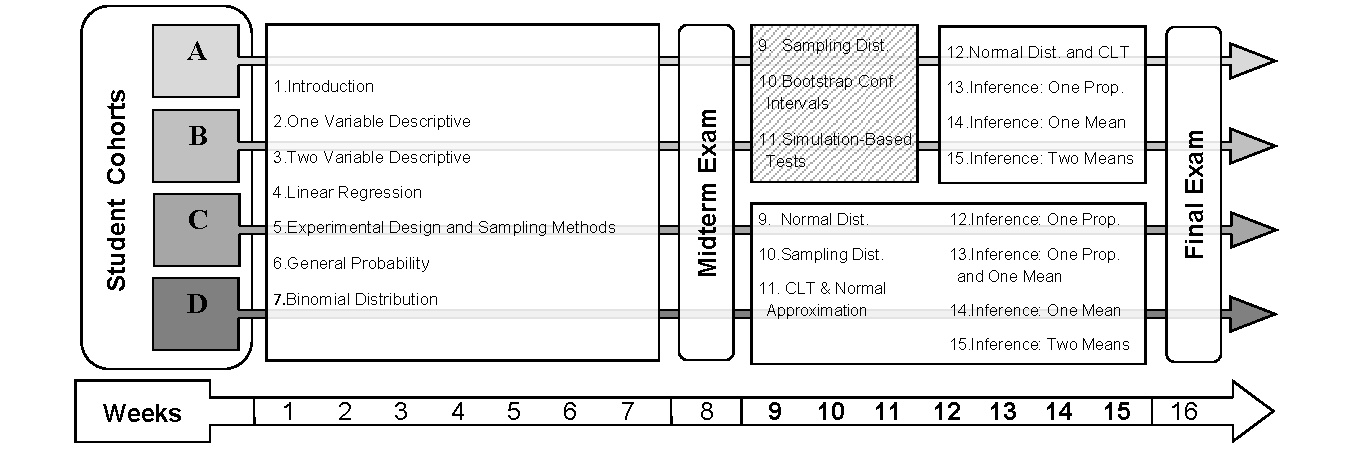
\includegraphics[keepaspectratio=true, width=1\textwidth]{CurriculumStudy/CurriculaPaths2.pdf}
\caption{\label{fig:CurricSched} Curricula Schedules}
\end{figure}

Cohorts C and D progressed through the traditional approach by first learning the normal distribution and use of the normal tables. They were then introduced to applications of the normal approximation within inference.  The traditional curriculum utilized simulation to display concepts, but only to the extent of demonstrating that sampling distributions can be approximated by normal distributions under certain conditions.  

During the second half of the semester the lectures, course note, homework and lab assignments differed between the two curricula.  However, homework and lab assignments were kept similar when they covered similar topics.  For example, all cohorts covered the topic of sampling distributions so the lab assignments were nearly identical between the two groups with the exception of a question pertaining to the normal approximation included for the traditional cohorts.  By the end of the semester all cohorts covered how to conduct inference using normal theory; however cohorts A and B additionally learned the core concepts of inference using simulation-based methods prior to learning traditional theory-based inference methods.  

%-----------------------------------------------------
\subsection{Experimental Design}
\label{design}

The logistics of administering a course with two distinct curricula and four cohorts of students required a well-structured design and creative scheduling on several fronts.  The primary objectives for the experimental design were to eliminate differences in non-inference related curriculum administration to the extent possible, remove the confounding instructor effect on each curriculum and to mitigate the effect of unknown lurking variables through random assignment of students to curricula.  

Students were randomly assigned to cohorts during the first week of the course.  Of the 101 students who completed the course and consented to the release of their data there were 50 students in the traditional treatment group and 51 students in the simulation-based treatment group. It is also worthwhile to note that of the 4 students to drop the course, all did so prior to week 9; thus, we can safely assume that the inference curriculum treatment did not play a role in the drop. All students who began the inference curricula completed the course.

Students were exposed to identical lecture and lab instruction for the first half of the semester and then diverge into two separate lecture and lab settings for the second half of the semester. This was done to make the experience as similar as possible such that both treatment groups would have the same exposure to terminology and ideas leading up to the inference topics. We could not reassign students to lecture and lab times different than the times for which they enrolled, which meant the logistics of the design required preemptive room scheduling and course time scheduling preparations.  By working with the department chair and course coordinator before students enrolled into sections, we were able to schedule two sections of the course to have identical lecture times but separate lab times. Special room scheduling was required because all students needed to attend the same lecture and lab rooms for the first half of the semester then split into separate lecture and lab rooms after the midterm.  This room and course time scheduling allowed for students to be divided into cohorts and attend the lecture or lab specific to their curriculum.  The lecture and lab room schedules for each cohort are displayed in Figure~\ref{fig:InstSched}.

\begin{figure}[hbtp]
\centering
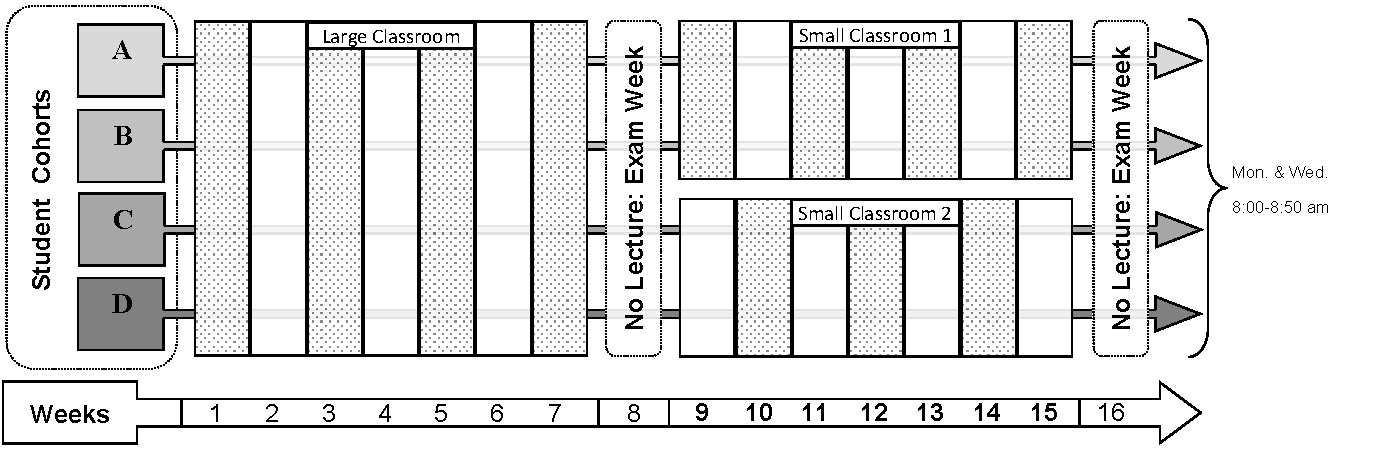
\includegraphics[keepaspectratio=true, width=1\textwidth]{CurriculumStudy/LectureInstructionWithRooms.pdf}\\
\vspace{.5cm}
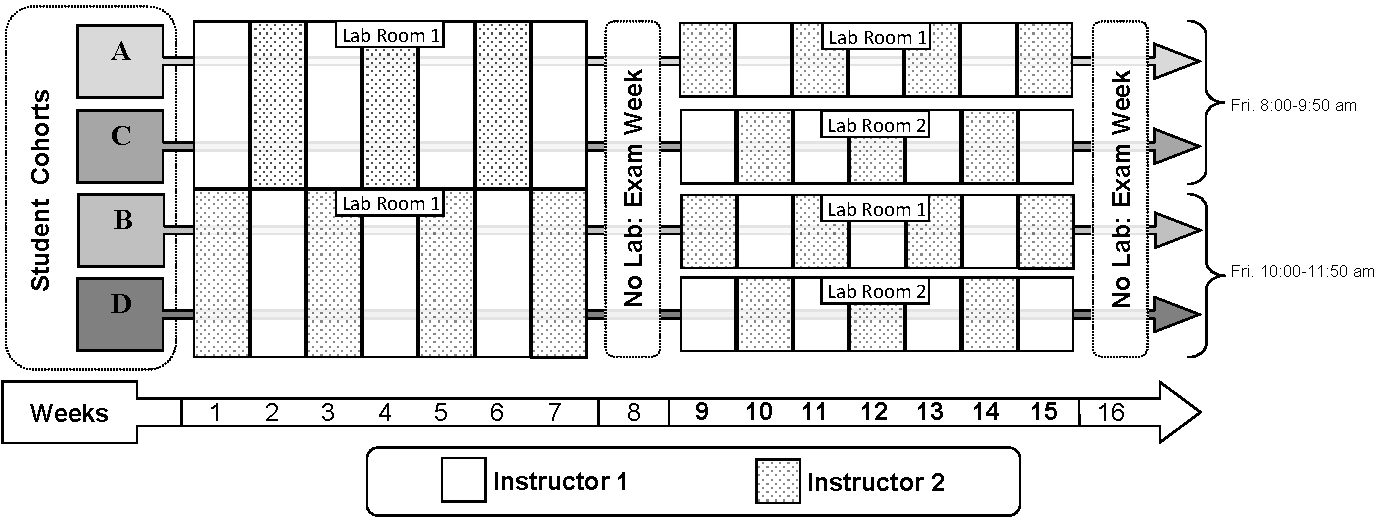
\includegraphics[keepaspectratio=true, width=1\textwidth]{CurriculumStudy/LabInstructionWithRooms.pdf}
\caption{\label{fig:InstSched} Instructor and Room Schedule}
\end{figure}


Assigning one instructor to each curriculum would confound the instructor effect and the curriculum effect.  To avoid confounding, each treatment group would need to receive instruction from both instructors.  An alternating weekly schedule was decided upon to spread out the instructor effects over both curricula. A coin was flipped to decide how to match the instructor to the curriculum when the alternation was initialized. The lecture and lab instruction schedules for each cohort can also be found below in Figure~\ref{fig:InstSched}. Note that each figure has student cohort and times fixed across all weeks, reflecting the unchanged time structure that each student enrolled into. The instructors and room locations are what changed throughout the course. 

%-----------------------------------------------------
\subsection{Data Collection}
\label{datacollect}

In order to measure learning outcomes for specific inference concepts we utilized question sets from the Assessment Resource Tools for Improving Statistical Thinking (ARTIST) for the topics of confidence intervals and hypothesis testing \citep{ARTIST}.  The ARTIST scaled question sets each consist of 10 multiple choice questions that are geared toward critical thinking about the inference topic.  These questions were administered as part of the written final exam for all students on the same day and time. The ARTIST scaled scores for the topics of confidence interval and hypothesis testing were recorded for each student. The multiple choice questions for the ARTIST scaled topics can be found in Appendix~\ref{appendA}.

The final exam also included two problems that tested the student's ability to conduct statistical inference in an applied setting using theory-based methodology. Each problem was based on a hypothetical scenario where data has been collected and inference needed to be conducted using the traditional approach using formulas and tables. The first problem provided data summaries and students needed to construct and interpret a confidence interval for a single population mean. The second problem required students to conduct a hypothesis test for a single proportion based on another set of data summaries. The applied inference problem scores for each student are not used for the primary analysis on learning outcomes but are included for an interesting peripheral analysis on student ability to conduct inference using traditional theory-based methods. The applied inference problems and grading rubrics can also be found in Appendix~\ref{appendA}. The exams were graded blindly, with no identifying information of the student or treatment visible during the grading process.

In addition to the ARTIST and applied inference question scores, data were collected from the first eight weeks of the course -- prior to student exposure to an inference curriculum. We have scores from homework assignments 1 to 7, lab assignments 1 to 7 and the midterm exam for each student. The midterm exam questions and grading rubrics can be found in Appendix~\ref{appMidtermExamQuestions}. Since all of these items were administered and graded equivalently for all students before being assigned to a curricula, the scores from these weeks will be referred to as the ``pre-treatment measurements''. Lastly, the data include the cohort to which each student belonged.

The research proposal approved by the Institutional Review Board specified that students' data would be entirely deidentified following the course, including all demographic information.  At the conclusion of the semester the data for the 101 students who consented to the release of their data were saved, with names and identity information removed, to a spreadsheet.  The deidentified student data was imported to \texttt{R} for the analysis described in Section~\ref{analysis} below. 


%-----------------------------------------------------
\subsection{Data Summary}
\label{dataSummary}

The ARTIST and applied inference question scores from the final exam are the response variables on which we wish to compare the groups of students from the two inference curricula. Figure~\ref{fig:ScoreHistsByGroup} displays the histogram, mean and standard deviation for each response variable, separated by curricula.  Midterm exam scores as also included in order to provide a comparison of the curricula groups using a pre-treatment measurement. 

\begin{knitrout}
\definecolor{shadecolor}{rgb}{0.969, 0.969, 0.969}\color{fgcolor}\begin{figure}[H]

{\centering \includegraphics[width=1\linewidth]{FigureScoreHistsByGroup-1} 

}

\caption[Histograms and summary statistics of scores separated by curricula group]{Histograms and summary statistics of scores separated by curricula group.}\label{fig:ScoreHistsByGroup}
\end{figure}


\end{knitrout}
\vspace{.05in}
In Figure~\ref{fig:ScoreHistsByGroup}, we see that the midterm exam scores are very similarly distributed for each group; with the traditional curriculum group scoring only slightly higher on average than the simulation-based curriculum group. This similarity is expected -- and desirable -- because the midterm was conducted prior to the treatment being administered, and the class materials and instruction were designed to be identical at that stage of the course.

Comparing the distributions in Figure~\ref{fig:ScoreHistsByGroup} we see that the simulation-based inference group had a higher average score than the traditional inference group on both of the ARTIST scaled question sets and on the applied confidence interval problem, but scored lower on average on the applied hypothesis testing problem.  The simulation-based inference group had lower variability than the traditional inference group on the ARTIST question set for confidence intervals, but higher variability on all other scores. These data summaries are suggestive of differences in the inference learning outcomes of the two groups. In Section~\ref{analysis}, we take a model-based approach to assess if these differences are statistically significant.




% 
% % latex table generated in R 3.0.2 by xtable 1.7-3 package
% % Mon Nov 24 15:50:03 2014
% 
% \begin{table}[ht]
% \small
% \centering
% \begin{tabular}{llrrrrr}
%   \hline
%     & Curriculum & Midterm & ARTIST CI & ARTIST HT & Applied CI & Applied HT \\ 
%   \hline
%   & Traditional & roomdat[1,3] & roomdat[1,4] & roomdat[1,5] & roomdat[1,6] & roomdat[1,7] \\ 
%    & Simulation & roomdat[2,3] & roomdat[2,4] & roomdat[2,5] & roomdat[2,6] & roomdat[2,7] \\ 
%  \hline
%  & & & & & &  \\ 
%  & & & & & &  \\ 
%  \hline
%   
%  Midterm Quartile & Curriculum & Midterm & ARTIST CI & ARTIST HT & Applied CI & Applied HT \\ 
%   \hline
% 1st Quartile & Traditional & 55.50 & 55.38 & 56.92 & 81.41 & 61.54 \\ 
%  & Simulation & 55.68 & 64.29 & 50.00 & 74.40 & 62.34 \\ 
%  & Difference & -0.18 & -8.90 & 6.92 & 7.01 & -0.80 \\ 
%  \hline
% 2nd Quartile & Traditional & 73.19 & 57.69 & 51.54 & 77.56 & 69.23 \\ 
%  & Simulation & 71.00 & 71.67 & 52.50 & 86.11 & 66.67 \\ 
%  & Difference & 2.19 & -13.97 & -0.96 & -8.55 & 2.56 \\ 
%  \hline
% 3rd Quartile & Traditional & 84.58 & 76.15 & 57.69 & 88.46 & 90.91 \\ 
%  & Simulation & 82.71 & 71.67 & 61.67 & 84.72 & 75.00 \\ 
%  & Difference & 1.87 & 4.49 & -3.97 & 3.74 & 15.91 \\ 
%  \hline
% 4th Quartile & Traditional & 94.33 & 78.33 & 65.83 & 90.97 & 93.94 \\ 
%  & Simulation & 91.67 & 82.50 & 76.67 & 95.83 & 93.18 \\ 
%  & Difference & 2.67 & -4.17 & -10.83 & -4.86 & 0.76 \\ 
%    \hline
% \end{tabular}
% \caption{Average percentage scores broken down by midterm exam quartiles.}
% \label{tab:examquartiles}
% \normalsize
% \end{table}



%---------------------------------------------------------------------------
\section{Analysis}
\label{analysis}

The primary goal of the analysis is to investigate if there is a curricula effect on inference concept learning outcomes.  Our data includes ARTIST scaled topic scores for confidence intervals and hypothesis tests which we use as the responses for the comparison of curricula. A model based approach is used to assess curricula effect while controlling for pre-treatment differences between students. With the two dimensional response and an assortment of covariates we employ a multivariate analysis of covariance (MANCOVA) model.   

Both curricula groups were required to learn how to conduct normal-based inference. This leads to another question of interest. Does the added simulation-based material turn out to be detrimental to student's ability to use distributional theory-based methods to conduct inference?  Two applied problems were included on the final exam that required students to use theory-based methods and formulas to conduct inference. These applied questions were used as the responses in a separate MANCOVA model to check for a curriculum effect. 

The bivariate MANCOVA models used for these two analyses are parameterized as 

\begin{eqnarray}\label{eq:mancova}
y_{i\ell} = \tau_{\ell} \mathbbm{1}_{\{i \in T\}} + \beta_{\ell 0} + \sum_{p=1}^{P}x_{ip}\beta_{\ell p} + \epsilon_{i\ell},
\end{eqnarray}
where 

\begin{tabular}{lp{5in}}
$y_{i\ell}$ &  is the $\ell^{th}$ response ($\ell \in \left\{1,2\right\}$) from  student $i$, $ 1 \le i \le n$,\\
$\tau_{\ell}$ & is the treatment effect of the simulation-based curriculum on response $\ell$, and \\
$\mathbbm{1}_{\{i \in T\}}$ & is an indicator function, that is one, if student $i$ is in the treatment group, and zero otherwise.\\
$\beta_{\ell 0}$ & is the common intercept for response $\ell$, and \\
$\beta_{\ell p}$, & $1 \le p \le P$ are the model coefficients of the $P$ covariates. \\
$x_{ip}$ & is the $p^{th}$ pre-treatment covariate score of student $i$, and\\
$\epsilon}_{i\ell}$ & is the error for the $\ell ^{th}$ response from the $i^{th}$ student. 
\end{tabular}

We assume that error pairs are independent and identically distributed:
\[
\vec{\epsilon}_{i} = 
\begin{bmatrix}
  \epsilon_{i1} \\ \epsilon_{i2} 
 \end{bmatrix}  
 \distas{iid} \text{MVN} \left( 
 \begin{bmatrix}
  0 \\ 0 
 \end{bmatrix},
 \Sigma = \begin{bmatrix}
  \sigma_{11}^2 & \sigma_{12}^2 \\ 
  \sigma_{21}^2 & \sigma_{22}^2
 \end{bmatrix}
 \right)
\]

% \begin{center}
% $y_{ik} = \tau_{k} \mathbbm{1}_{\{i \in T\}} + \beta_{0k} + \Bigg(\sum_{p=1}^{P}x_{ip}\beta_{pk}\Bigg) + \epsilon_{ik}$,\\
% 
% where $k \in \left\{1,2\right\}$,  $i \in \left\{1,...,n\right\}$, and $p \in \left\{1,...,P\right\}$,
% 
% $\vec{\epsilon}_{i} = 
% \begin{bmatrix}
%   \epsilon_{i1} \\ \epsilon_{i2} 
%  \end{bmatrix}  
%  \distas{iid} $ MVN$\left( 
%  \begin{bmatrix}
%   0 \\ 0 
%  \end{bmatrix},
%   \begin{bmatrix}
%   \sigma_{11}^2 & \sigma_{12}^2 \\ 
%   \sigma_{21}^2 & \sigma_{22}^2
%  \end{bmatrix}
%  \right)$,
% \end{center}

With this parameterization, it is clear that the underlying structure of the MANCOVA model is a multivariate multiple linear regression that can include categorical and continuous covariates. Note that the paired error terms from each student are correlated but are specified as independent between students. The assumption of independence between student response scores is understood to be unrealistic for students from the same class. \km{The repercussions of violating the assumption of independence between student responses will be explored through a simulation study in Section~\ref{SimStudy} following the analysis.}

%-----------------------------------------------------
\subsection{Modeling ARTIST Outcomes}
\label{ArtistModel}

We begin with the model for the ARTIST scaled topic scores.  Many of the pre-treatment variables are highly correlated. To select a model with only the most predictive pre-treatment covariates, model selection was conducted by first running backward selection based on AIC then removing further covariates that posed collinearity issues. The model selected for final analysis included three covariates: an indicator variable for the curriculum treatment group, the lab 5 score and the midterm score.  The midterm tested students on materials from weeks 1-7 and lab 5 assessed understanding of topics related to random selection techniques.  We will refer to this selected model as the ``ARTIST Model''. Model fit for the ARTIST Model was assessed to be satisfactory; see Appendix~\ref{appARTISTModDiag} for residual plots and other model diagnostics.





To test for overall covariate effects on the multivariate responses we use Pillai's $\Lambda$. Table~\ref{tab:overallmod} shows a weak overall effect of the curriculum treatment on the paired ARTIST scaled topic scores.  This prompts us to investigate the treatment effect on the ARTIST scaled topic scores for confidence intervals and hypothesis tests separately, to see if the weak overall effect is driven by a significant effect on one of the two scores.

\begin{table}[hbtp]
\centering
\begin{tabular}{lrrr} \hline
 & Pillai's $\Lambda$ & Approx. F & Pr($>$$|$F$|$)\\ 
 \hline  
Midterm & 0.2109 & 12.8277 &
0.0000\\ 
Lab 5 & 0.0792 & 4.1261 &
0.0191\\ 
Treatment & 0.0469 & 2.3605 &
0.0998\\ 
\hline
\end{tabular}
\caption{Tests for overall covariate effects on ARTIST question scores using Pillai's $\Lambda$.}
\label{tab:overallmod}
\end{table}

To investigate the effect of the curriculum treatment on each ARTIST scaled topic score, we analyze the two underlying linear models that comprise the overall MANCOVA model. Table~\ref{tab:cimod} displays the coefficients of the linear model fit to the ARTIST scaled score for confidence interval learning outcomes along with covariate ranges to provide context to coefficient magnitudes. It should be noted that although the midterm and lab scores were recorded discretely, they were treated as continuous covariates when fitting the model. We find that midterm, lab 5 and the curriculum treatment effect are significant. Specifically, the simulation-based inference group scored significantly higher by 0.7149 out of a possible 10 points, a 7.146\% improvement in confidence interval learning outcomes on the ARTIST scale while controlling for midterm and lab 5 scores.\\


% latex table generated in R 3.0.2 by xtable 1.7-3 package
% Tue Jul 29 15:46:21 2014
\begin{table}[hbtp]
\centering
\begin{tabular}{rccc}
  \hline
 & Covariate Values & Estimate & 95\% Confidence Interval \\ 
  \hline
Intercept & 1 & 1.4648 & ( -0.5467 , 3.4763 ) \\ 
  Midterm & \{0,1,...100\} & 0.0477 & (  0.0253 , 0.0701 ) \\ 
  Lab 5  &  \{0,1,...100\} & 0.0183 & (  0.0057 , 0.0309 ) \\ 
  Treatment &  \{0,1\} & 0.7146 & (  0.0435 , 1.3858 ) \\ 
   \hline
\end{tabular}
\caption{Coefficients for model fit to ARTIST score for confidence interval topic.}
\label{tab:cimod}
\end{table}

Table~\ref{tab:htmod} displays the coefficients of the linear model fit to the ARTIST scaled score for hypothesis test learning outcomes.  We find that only the midterm score is significant for predicting learning outcomes for hypothesis testing. There was no significant curriculum treatment effect. \\

% latex table generated in R 3.0.2 by xtable 1.7-3 package
% Tue Jul 29 15:41:44 2014
\begin{table}[hbtp]
\centering
\begin{tabular}{rccc}
  \hline
 & Covariate Values & Estimate & 95\% Confidence Interval \\ 
  \hline
Intercept & 1 & 2.1053 & ( 0.0046 , 4.2060 ) \\ 
  Midterm & \{0,1,...100\} & 0.0386 & (  0.0152 , 0.0620 ) \\ 
  Lab 5  &  \{0,1,...100\} & 0.0085 & (  -0.0046 , 0.0217 ) \\ 
  Treatment &  \{0,1\} & 0.3050 & (  -0.3960 , 1.0059 ) \\ 
   \hline
\end{tabular}
\caption{Coefficients for model fit to ARTIST score for hypothesis test topic.}
\label{tab:htmod}
\end{table}



A final consideration in the comparison of learning outcomes using the ARTIST model is that we made two primary comparisons; the curriculum effect on each of the inference topics. While several multiple comparisons adjustments have been developed for univariate response modeling, the Bonferroni method is the only traditional adjustment that is flexible enough for use in the MANCOVA setting. With the Bonferroni adjustment, if we wish to maintain an overall $\alpha=0.05$ significance level then we hold each individual comparison to the $\alpha=0.025$ level. After using the Bonferroni adjustment, the curriculum effect on learning outcomes for confidence interval topics would no longer considered significant ($\text{p-value} = 0.031 > 0.025$) at the overall $\alpha = 0.05$ level, but instead would be significant at the overall $\alpha = 0.1$ level.  However, the Bonferroni method is well known for being overly conservative in its adjustment, and we are comfortable with maintaining the original interpretations.

%-----------------------------------------------------
\subsection{Modeling Applied Theory-Based Inference Scores}
\label{AppliedModel}

As with the MANCOVA model for ARTIST scaled question scores, we consider all pre-treatment measurements in a new model for the two applied theory-based inference question scores.  Backward stepwise selection was used to obtain a reduced MANCOVA model in a model selection process identical to that described in Subsection~\ref{ArtistModel}. We will refer to the selected model here as the ``Applied Model''.  Residual plots and other model diagnostics for the Applied Model may be found in Appendix~\ref{appAppliedModDiag}.

Table~\ref{tab:overallmod1} shows -- based the Pillai's $\Lambda$ -- that there was no overall effect of curriculum treatment on the scores for the pair of applied inference problems. This is of particular interest because students receiving the simulation-based curriculum had three weeks less of coursework involving the use of normal distributions and normal tables. This implies that despite the increased complexity of the simulation-based material and the shortened exposure to theory-based inference concepts, there was no significant detriment to students' performance in conducting inference using theory-based methods. It should be noted that the applied questions from the final exam were written by the authors and have not been assessed as reliable metrics for learning outcomes. Thus, the results are reported as supplementary to the discussion on learning outcomes measured by the ARTIST scaled topics.



\begin{table}[hbtp]
\centering
\begin{tabular}{lrrr} \hline
 & Pillai's $\Lambda$ & Approx. F & Pr($>$$|$F$|$)\\ 
 \hline  
Midterm & 0.3238 & 22.9881 &
0.0000\\ 
Homework 2 & 0.0870 & 4.5750 &
0.0127\\ 
Treatment & 0.0108 & 0.5217 &
0.5952\\ 
%Treatment & round(summarytab1[4,2],4) & round(summarytab1[4,3],4) &
%round(summarytab1[4,6],6)\\ 
\hline
\end{tabular}
\caption{Tests for overall covariate effects on Applied question scores using Pillai's $\Lambda$.}
\label{tab:overallmod1}

\end{table}



\km{
%-----------------------------------------------------
\subsection{Model Assessment}
\label{SimStudy}

The bivariate MANCOVA models that were employed in Sections~\ref{ArtistModel}~and~\ref{AppliedModel} make the assumption of independent errors between students; an assumption which is very likely violated in practice because learning outcomes for students attending the same lectures and labs are very likely related. The assumption of independence is typically made for convenience and the lack of repetition on the lecture and lab levels prevents us from estimating a proper variance structure. It is therefore important to assess the consequences of this violation on the fitted MANCOVA model; specifically, the impact on the Type 1 error rates in tests for curriculum effects on learning outcomes. We elect to explore the consequences through a simulation study wherein the assumption of independence is knowingly violated and the effects on errors rates can be recorded.}

\km{We choose the ARTIST Model (\ref{eq:mancova}) from Sections~\ref{ArtistModel} as the basis for our simulation study. Under the assumption of independence between students, we found weak evidence of a curriculum effect on the bivariate ARTIST learning outcomes using Pillai's test. Further inspection of the individual responses using t-tests revealed significant evidence of a curriculum effect on confidence interval learning outcomes, but no evidence of a curriculum effect on hypothesis test learning outcomes. In order to assess the trustworthiness of the results, we must first know how a violation of the assumption of independence impacts the Type 1 error rates for these tests. We simulate responses from a generative model without a curriculum effect on learning outcomes (i.e.\ $\tau_{1} = \tau_{2} = 0$) and where the assumption of independence between students is violated to a known degree. We then track the Type 1 error rate in curriculum effects when the ARTIST model, assuming independence, is fit to the simulated responses.}

\km{The generative model for the simulations is adapted from the MANCOVA model~(\ref{eq:mancova}) by adding random effects to violate the independence between students. The generative model includes fixed effects for lab 5 and midterm scores, and random effects for responses to each ARTIST topic, lab sections and lecture section. Recall that responses are nested within students, students are nested within lab sections, and labs are nested within lecture sections. Thus the generative model is defined as,
%
\begin{eqnarray}\label{eq:simgenerative}
y_{ijk\ell} = \left[ \beta_{0k} + x_{ijk1}\beta_{k1} + x_{ijk2}\beta_{k2} \right] + \left[ \eta_{\ell} + \gamma_{k\ell} + \delta_{jk\ell} + \epsilon_{ijk\ell} \right],
\end{eqnarray}
%
for $i \in \left\{1,\dots,n\right\}$, $j \in \left\{1,2,3,4\right\}$, $k \in \left\{1,2\right\}$, and $\ell \in \left\{1,2\right\}$.  Where $y_{ijkl}$ is the $\ell^{th}$ response from student $i$ who is in lab section $j$ and lecture section $k$. The fixed effects portion of the model, within the first square brackets, is defined identically to the original ARTIST model~(\ref{eq:mancova}). In the generative model the $\beta$ coefficients are set equal to the corresponding coefficient estimates from the original ARTIST model. The remaining terms, $\eta_{\ell}$, $\gamma_{k\ell}$, $\delta_{jk\ell}$, and $\epsilon_{ijk\ell}$ are random effects for responses, lecture sections, lab sections and individual errors, respectively, are defined as
%
\[
\vec{\epsilon}_{ijk} = 
\begin{bmatrix}
  \epsilon_{ijk1} \\ \epsilon_{ijk2} 
 \end{bmatrix}  
 \distas{iid} \text{MVN} \left( 
 \begin{bmatrix}
  0 \\ 0 
 \end{bmatrix},
 \Sigma = \begin{bmatrix}
  \sigma_{11}^2 & \sigma_{12}^2 \\ 
  \sigma_{21}^2 & \sigma_{22}^2
 \end{bmatrix} 
 \right),
\]
\[
\vec{\delta}_{jk} = 
\begin{bmatrix}
  \delta_{jk1} \\ \delta_{jk2} 
 \end{bmatrix}  
 \distas{iid} \text{MVN} \left( 
 \begin{bmatrix}
  0 \\ 0 
 \end{bmatrix},
 d\Sigma = \begin{bmatrix}
  d\sigma_{11}^2 & d\sigma_{12}^2 \\ 
  d\sigma_{21}^2 & d\sigma_{22}^2
 \end{bmatrix} 
 \right),
\]
\[
\vec{\gamma}_{k} = 
\begin{bmatrix}
  \gamma_{k1} \\ \gamma_{k2} 
 \end{bmatrix}  
 \distas{iid} \text{MVN} \left( 
 \begin{bmatrix}
  0 \\ 0 
 \end{bmatrix},
 g\Sigma = \begin{bmatrix}
  g\sigma_{11}^2 & g\sigma_{12}^2 \\ 
  g\sigma_{21}^2 & g\sigma_{22}^2
 \end{bmatrix} 
 \right),
\]
\[
\vec{\eta} = 
\begin{bmatrix}
  \eta_{1} \\ \eta_{2} 
 \end{bmatrix}  
 \distas{iid} \text{MVN} \left( 
 \begin{bmatrix}
  0 \\ 0 
 \end{bmatrix},
 z\Sigma = \begin{bmatrix}
  z\sigma_{11}^2 & z\sigma_{12}^2 \\ 
  z\sigma_{21}^2 & z\sigma_{22}^2
 \end{bmatrix} 
 \right).
\]

Thus the variance structure for the responses includes common variance components $\sigma_{\ell\ell'}$ and scaling parameters $z$, $g$ and $d$. The variance components for $\sigma_{\ell\ell'}$ from the original ARTIST model are plugged in as variance parameters for the generative model. The scaling parameter $z$ controls the variability that is common between all student responses; thus $z \sigma_{\ell\ell'}$ is the covariance of responses for ARTIST sets $\ell$ and $\ell'$ between students that do not share lecture or lab sections. The scaling parameter $g$ controls the additive increase to covariance between students of the same lecture section, $g \sigma_{\ell\ell'}$, and $d$ controls the additive increase to covariance between students of the same lab section, $d \sigma_{\ell\ell'}$. If each of these variance scaling parameters is set to zero, there is no violation to the assumption of independence between students; thus making the variance structure of the generative model~(\ref{eq:simgenerative}) match the error structure of the original ARTIST model~(\ref{eq:mancova}). However, these parameters may be adjusted to violate the independence assumption to different degrees.}

\km{The simulation procedure for assessing the Type 1 error rates under violations of independence between student responses is conducted through a five step process. We consider violations based on all combinations of $d \in \{0,0.02,0.04,0.06,0.08,0.1\}$ and $g \in \{0,0.02,0.04,0.06,0.08,0.1\}$. We set $z$=0 for all simulations because any random effect that is common to \textit{all} students will not effect tests for curriculum effects (i.e. the difference in average responses between curricula groups remains constant). For each combination of variance scaling parameters we repeat the following simulation process for $m \in \{1,\dots,20000\}$: 
%
\begin{enumerate}
\item Randomly permute the lecture and lab section labels in the data 
\item Simulate the random effects by drawing $\vec{\epsilon_{ijk}}^{\hspace{.1cm}(m)}$, $\vec{\delta_{jk}}^{\hspace{.1cm}(m)}$,$\vec{\gamma_{k}}^{\hspace{.1cm}(m)}$, and $\vec{\eta}^{\hspace{.1cm}(m)}$ from the multivariate normal distributions defined above.
\item Compute the $m^{th}$ simulated responses with generative model~(\ref{eq:simgenerative}) as:
%
\begin{center}
$y_{ijk\ell}^{\hspace{.1cm}(m)} = \beta_{0k} + x_{ijk1}\beta_{k1} + x_{ijk2}\beta_{k2} + \eta_{\ell}^{\hspace{.1cm}(m)} + \gamma_{k\ell}^{\hspace{.1cm}(m)} + \delta_{jk\ell}^{\hspace{.1cm}(m)} + \epsilon_{ijk\ell}^{\hspace{.1cm}(m)}$
\end{center}
%
\item Fit the ARTIST Model, assuming independence, to the simulated responses.
\item Conduct Pillai's test for overall curriculum effect, then t-tests for curriculum effect on each response individually. Record test statistics and p-values.
\end{enumerate}
}

\km{Recall that in the generative model~(\ref{eq:simgenerative}) does not include a treatment effect, therefore any test where significant curriculum effects are found has incurred a Type 1 error. Figure~\ref{fig:simerrorratesdg} displays the observed Type 1 error rates in simulations under violations of independence between students. When the variance scaling parameters are set to zero there is no violation of independence and we see that tests hold at the nominal Type 1 error rate of $\alpha$=0.05. However, the error rates increase quickly when the variance scaling parameters, $d$ and $g$, increase. This occurs more dramatically for the overall Pillai's test than for the individual t-tests.}

\km{To establish points of reference for interpreting Figure~\ref{fig:simerrorratesdg} we examine the error rates under a few specific parameter settings. When the between labmate covariance is 4\% higher than for non-labmates (i.e. $d$=0.04 and $g$=0) the Type 1 error rates for individual t-tests are above 0.15 and the Pillai's test is above 0.20; over three and four times the nominal rate, respectively. Worse, when the between classmate covariance in 4\% higher than for non-classmates (i.e. $d$=0 and $g$=0.04) the Type 1 error rates for individual t-tests are above 0.25 and the Pillai's test is above 0.35; over five and seven times the nominal rate, respectively. This error rate inflation occurs because the random effects based on lecture and lab sections are being misinterpreted in the ARTIST model as fixed effects of curriculum due to the assumption of independence between students; a misinterpretation made worse in the case of lecture section due to the complete confounding with curriculum.}

\begin{knitrout}
\definecolor{shadecolor}{rgb}{0.969, 0.969, 0.969}\color{fgcolor}\begin{figure}[h]

{\centering \includegraphics[width=1\linewidth]{Figuresimerrorratesdg-1} 

}

\caption[Type 1 error rates from 20,000 simulations under each combination of ]{Type 1 error rates from 20,000 simulations under each combination of $d$ and $g$ for individual t-tests and Pillai's overall test for curriculum effects on the ARTIST response scores. The horizontal black line indicates the nominal Type 1 error rate of $\alpha$ = 0.05.}\label{fig:simerrorratesdg}
\end{figure}


\end{knitrout}

\km{Note that the magnitude of variance scaling parameters is necessarily attributed to non-curricular factors because the generative model is designed to carry no curriculum treatment effect. Great care was taken during the study design and administration to minimize all non-curricular differences that students encountered in lecture and lab sections; using the alternation of instruction, identical curricula administered with all students in the same room in weeks 1 to 8, and careful pedagogical preparation. However, the simulation study indicates that even in the case of very minor lecture or lab based variance structure the model suffers highly inflated Type 1 error rates and gives rise to major doubts about the results of tests for curricular effects discussed in Sections~\ref{ArtistModel} and~\ref{AppliedModel}.}

\km{
%---------------------------------------------------------------------------
\section{Discussion and Conclusions}
\label{discussion}

The ARTIST model analysis indicates that students receiving the simulation-based curriculum have significantly higher learning outcomes for confidence interval related topics. The magnitude of the improvement was 7.146\% on the ARTIST scale, after accounting for the midterm and lab 5 scores. There was no significant difference between traditional and simulation-based curricula on learning outcomes for hypothesis test topics. There are however several issues that merit serious concern and consideration about the validity of these results; including the model assumption of between student independence, the diverse population of interest, the replicability of treatments, and the measurement of learning outcomes. }

\km{The experimental design used randomization of individual students to curricula to aid in the creation of homogeneous groups receiving each the curricular treatment, but the treatments were administered on the lecture and lab section level. The bivariate MANCOVA model was fit under the assumption of independence between students because the lack of repetition in lecture and lab sections does not allow for proper estimation of lecture or lab based variance structure. Even when great efforts are made to control for non-curricular differences in the student experiences, as was done in this study, it is unreasonable to assume that students of the same lecture and/or lab sections would not share some degree of non-curricular connection in learning outcomes as a result of having shared the same physical learning environment. The simulation study indicates that even minor violations of this assumption leads to unacceptable inflation to Type 1 error rates in tests for curriculum effects. }

\km{This error rate inflation is a major problem not only for this study, but every educational study where curricular treatments are implemented in groups of students but comparisons are made between learning measurements from individual students. Alternative experimental designs could implement curricular treatments on the individual student level or have sufficient group replication to make comparisons on the group level; each option suffering major logistical and resource demands. To overcome this issue, a deeper understanding of inter-student variability is needed to support the use of more appropriate covariance structures. Uniformity trials are an established method within agricultural statistics that examine variance structure through experiments with only a single treatment \citep{richter2012geostatistical}. If applied in a classroom setting, this approach provides a potential avenue to identify variance structures that form due to student cohorts, which could then be used to choose reasonable plug-in estimates for variance components in studies without cohort repetition. This would require a widespread and concerted effort by many in the discipline to collect and catalog data on inter-student variance structure from many classroom scenarios. }

We must also bear in mind the population for which the results of this study may be representative. The study was conducted with undergraduate students enrolled in an introductory statistics course at a large public Midwestern university.  The course is required for students in agricultural and biological sciences.  Students in the course are predominantly sophomores and juniors. The results are therefore only applicable to the extent to which these students represent the broader population of introductory statistics students.

% The experimental design bolsters the establishment of a causal effect through utilization of control of non-inferential course components and random assignment of students to treatment groups.  There are two assumptions that we must make to justify a claim of causality.  We must assume that the random assignment successfully eliminated all possible lurking variables (i.e. student demographic and educational backgrounds); however this is the assumption made by most randomized experiments. We must also make the assumption that the instructor effect on learning outcomes has been eliminated by the weekly alternation of instructors. We believe both assumptions are justifiable due to the care taken with randomization and instruction alternation.  

%An issue that is more problematic than the assumptions made about causality is that 
\km{Another important consideration is that the treatment itself was a half semester curriculum -- a highly complex combination of lesson plans, lecture content, assignments and technology use. The treatment complexity poses a problem in identifying precisely which, if any, components of the curriculum might improve learning outcomes. Investigation of the efficacy of the individual components from the improved curriculum is an area for future research. 
%The simulation-based approach to inference that we employed achieved a significant improvement in measured learning outcomes related to confidence intervals, but 
There are also many possible ways to implement simulation-based inference within a course. One noteworthy characteristic was that the simulation-based curriculum that was employed in this study utilized bootstrapping to teach the concepts of confidence intervals as opposed to inverting a simulation-based hypothesis test. This study does not attempt to identify if all possible implementations of the simulation-based approach would achieve improvements in learning outcomes. }

\km{A surprising aspect of the results is that the curriculum effect was more pronounced for the learning outcomes of confidence interval topics than for hypothesis testing topics. It is surprising because much of the literature on the simulation-based approach is focused on the theoretical benefits in simplifying the concepts of hypothesis testing. A potential explanation is that the benefits of the simulation-based methods were counterbalanced by the challenge faced when students were also required to learn theory-based methods; forcing them to mentally reconcile the differences between how each approach obtains a p-value. It is important to recall that due to departmental requirements for the course, the treatment group learned simulation-based inference in addition to an abbreviated unit on theory-based inference methods. However, based on the highly inflated Type 1 error rates in studies with cohort based variance structure, it is also very plausible that the disparity seen is purely random. }

%The simulation-based curriculum lead to no significant difference in learning outcomes for hypothesis testing on the ARTIST scale, despite the added complexity of learning additional concepts for conducting simulation-based tests. In addition, the added complexity related to bootstrapping confidence intervals appears to have actually improved learning outcomes for confidence intervals on the ARTIST scale. The transition between approaches may have simply been easier for confidence interval topics; the primary difference being that the bootstrap estimated standard error was replaced by a simple theory-based estimator of the standard error. 

The evidence of improved learning outcomes is also contingent on the efficacy of the ARTIST scales to measure student learning. The ARTIST question sets have been criticized as being increasingly outdated and for lacking reliability and validity evidence \citep{Ziegler2014}. The Comprehensive Assessment of Outcomes in Statistics (CAOS; \citealt{DelMas2007}) was considered as alternative assessment of student learning because it is nationally normed and backed by a reliability study; however, the reliability was assessed for the CAOS test in its entirety (40 items) which was decided to be too extensive to be administered in addition to the other necessary components on the final exam. The Reasoning about P-values and Statistical Significance (RPASS; \citealt{LaneGetaz2013}) assessment was also considered, but not selected, because it does not assess learning outcomes for confidence interval related topics. The Basic Literacy in Statistics (BLIS; \citealt{Ziegler2014}) and the Goals and Outcomes Associated with Learning Statistics (GOALS; \citealt{Garfield2012}) assessments were recently designed to better measure student learning in the contemporary statistics classroom, unfortunately these assessments were in development at the time of this study.

\km{ This study is unable to draw reliable conclusions on the efficacy of simulation-based methods for teaching statistical inference due to the volatility of the Type 1 error rates under minor violations to model assumptions. This is a fundamental problem for all comparative educational studies where pedagogical treatments are administered on the class level and measurements are taken the individual student level. Viewed as a case study of two curricula administered within extremely similar student groups, we found that simulation-based curriculum had a noticeable improvement in learning outcomes associated with confidence intervals and a small improvement in learning outcomes associated with hypothesis testing. While the results are clearly not conclusive in assessing the curricular effect on learning outcomes, the findings do merit further consideration into the pedagogical benefits of a simulation-based curriculum. }
\chaptocbreak

\chapter{A SHINY NEW OPPORTUNITY FOR INTERACTION WITH BIG DATA IN UNDERGRADUATE EDUCATION}\label{ShinyDBSampler}




%opening
%\title{A \texttt{shiny} New Opportunity for Interaction with Big Data in Undergraduate Education}
%\subtitle{ }
%\author{Karsten Maurer \\ Iowa State University, Ames, IA, USA}

% \date{Received: date / Accepted: date}

 
\begin{center}
\textbf{Status}: In Preparation for Submission to \textit{Technology Innovations in Statistics Education} (TISE)\\
\end{center} 

\begin{center}
\textbf{Authors}\\
Karsten Maurer, Iowa State University, Primary Author\\
Heike Hofmann, Iowa State University\\
\end{center}


\begin{center}
\textbf{Abstract}\\
\end{center}

As the availability of truly massive data proliferates, it is enticing to incorporate these data sets into the curriculum of an undergraduate statistics course.  Major barriers exist for interacting with big data due to the computationally intense nature of working with large databases.  Difficulties include gaining access to databases, interacting with database management software, and obtaining summary statistics or manageable subsamples from the database for student use.  This paper describes a web-based software application, the \textit{Shiny Database Sampler}, which allows instructors and students to bypass these barriers using a simple point-and-click interface constructed through \texttt{R} and the \texttt{R} packages \texttt{shiny} and \texttt{RMySQL}. The Shiny Database Sampler allows instructors and students to obtain subsamples from databases, using a variety of random sampling schemes. Application and evaluation of the software indicate that students find the interface easy to use, well connected to course concepts, and engaging through access to real data.

%-----------------------------------------------------------

\section{Introduction}

Statistics education has been rapidly evolving in the past decade with respect to undergraduate course curriculum and assessment. Technology has played the role as a catalyst for many of these major changes. An important change involves how data is accessed and analyzed in the classroom. The GAISE report \citep{GAISEcollege} laid out six recommendations on how to improve the teaching of introductory statistics; two of which urge statistics instructors to ``Use technology for developing conceptual understanding and analyzing data'' and to ``Use real data''. There are many software tools and online repositories for instructors to access real data for use in the statistics classroom. These include the Data and Story Library \citep{DASL} and its Australian counterpart, OzDASL \citep{OzDASL}, the Data Archives of the Journal of Statistics Education \citep{JSErepo}, CAUSE Web Repository \citep{CAUSErepo}, and Many Eyes \citep{ManyEyes}. These repositories are wonderful for accessing many real data sets but the majority of the data sets currently available are quite small in scale.

\citet{Finzer2007} argue that in curricula for introductory level statistics ``(w)hat seems to us to be missing are data sets-especially large and highly multivariate data sets-that are ripe for exploration and conjecture driven by the students' intrigue, puzzlement and desire for discovery'' \citep[p.1]{Finzer2007}. Large, real data sources are becoming increasingly available, but tend to be less easily accessible. A major contributor to this trend is the Freedom of Information Act which to ensures that non-classified data from the United States government is publicly available \citep{FOIA}. The online government resources at \url{www.data.gov/} \citep{DataGov}, \url{www.census.gov/} \citep{Census}, \url{www.nhtsa.gov/} \citep{NHTSA} and \url{www.cdc.gov/} \citep{CDC} are all locations of massive data stores. Governmental data sets contain rich information related to many socially relevant issues, making them prime candidates for engaging student interest.

The goal of connecting undergraduate statistics students with big data sources requires careful consideration to implement. \citet{jacobs2009} speaks of the difficulties associated with using, ``data whose size forces us to look beyond the tried-and-true methods that are prevalent at that time'', including scaling computational tasks, avoiding sub-optimal storage schemes and parallel processing.

New data technologies are needed in order to allow introductory statistics students to interact with big data sources, such as the governmental databases. This paper discusses the construction and functionality of the Shiny Database Sampler; a web-based application that allows students to pull random samples from large databases. Then, details of the implementation within a lab assignment and course project for an introductory statistics course are discussed. Lastly, the survey responses from 265 introductory statistics students whom used the Shiny Database Sampler for the lab assignment are analyzed to evaluate the software.

%-----------------------------------------------------------------------------------
\section{Shiny Database Sampler}

Exposing students to larger and larger data is tricky because it becomes increasingly unwieldy to transfer, store and access data on student's personal computers. Access through remote databases and database querying languages is outside the realm of comfort for both students and instructors in most undergraduate statistics courses. The Shiny Database Sampler is a simplified graphical user interface that is designed to allow students to take appropriately sized subsets from the databases to practice small sample methodology taught in most introductory statistics courses. Working with a small static subset from the large database would let the remainder of the database go to waste. Instead the tool allows students to specify a random sampling scheme that will pull the subset from database dynamically. This is done to emphasize the role of random sampling techniques in data collection, an important concept within an introductory statistics curriculum.

%%%-----------------------------------------------------------------------------------
\subsection{Layout and Design}

The Shiny Database Sampler allows the user to randomly sample subsets from remotely stored SQL databases using a point-and-click graphical user interface. The tool is available online through the link at \url{http://shiny.stat.iastate.edu/karstenm/ShinyDatabaseSampler/}. A screenshot of the graphical user interface is shown in Figure~\ref{fig:samplesummarizetab}.  %; however these sections contain different options and displays depending on which tab of the application is selected.\\

The Shiny Database Sampler is a JavaScript based online application created using the \texttt{shiny} package \citep{shiny} in the statistical computing language \texttt{R} \citep{R}. The Shiny package uses \texttt{R} code files to generate the graphical user interface in a web browser that interacts with an \texttt{R} session running on the server.  It is used in combination with the \texttt{RMySQL} package \citep{RMySQL} to allow the \texttt{R} session on the server machine to query the database at the user's request via buttons in the graphical user interface.

The interface was designed with a focus on the quality of the software as an educational tool. The field of software development defines six attributes contributing to software quality: functionality, reliability, usability, efficiency, maintainability, efficiency and portability (\citealt{bevan1997quality}; \citealt{manuel2002quality}). The Shiny Database Sampler is highly portable, as it can be accessed online through any JavaScript enabled web browser. The reliability and maintainability of \texttt{shiny} applications depend upon proper implementation of \texttt{R} and \texttt{shiny} on the web server. The key consideration with respect to efficiency is to optimize the database querying using proper indexing so that sample retrieval occurs almost instantaneously \citep{schwartz2012high}. 

The graphical user interface contains two tabs, each broken into two panels. The layout is designed for the user to select actions in the side panel and view the results in the main panel. The functionality and usability of the \textit{Sample and Summarize} and \textit{Visualize} tabs are discussed in the following subsections. 

\subsubsection{The \textit{Sample and Summarize} tab}
%\paragraph{The ``Sample and Summarize'' tab} \hfill\newline

A screenshot of the interface for the \textit{Sample and Summarize} tab is shown in Figure~\ref{fig:samplesummarizetab} below. A sidebar panel which contains all the sampling options and controls, and a main panel which contains the data table and brief summary of the sampled data set.

\begin{figure}[hbtp]
\centering
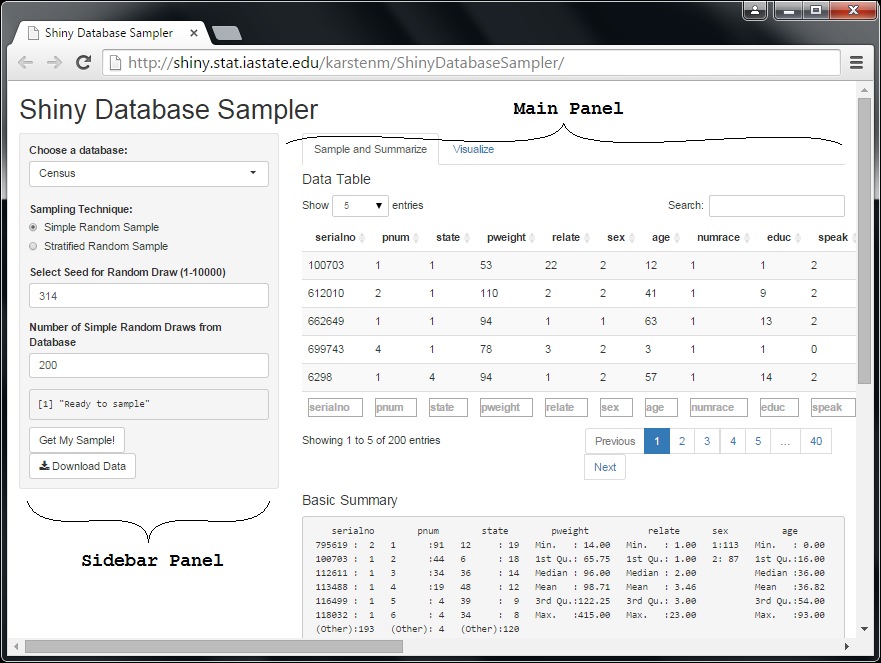
\includegraphics[keepaspectratio=TRUE,width=.95\textwidth]{ShinyDBSampler/SampleAndSummarizeWithPanelLabels.png}
\caption{Shiny Database Sampler Layout for \textit{Sample and Summarize} Tab} 
\label{fig:samplesummarizetab}
\end{figure}

The sidebar panel contains several fields and buttons for selecting and executing a sampling plan.  At the top of the sidebar is a drop-down menu to select the database table from which the user may take a random subsample.  The current version of the tool allows users to access the 2001-2009 Fatality Analysis Recording System accident data from the National Highway Traffic Safety Administration (\url{www.nhtsa.gov/FARS}) and the Public Use Micro Sample data from the 2000 United States Census (\url{www.census.gov/}).

After selecting the database, the user can choose between taking a simple or stratified random subsample of data from the database. If the user chooses simple random sampling, then they must specify a sample size; whereas if the user chooses stratified random sampling the strata variable and number of observations per stratum need to be specified. Lastly the user sets the seed for the selection algorithm. Setting the seed may seem to contradict the intention to draw random subsets, however it was included after careful consideration. For classroom settings, it is often desirable for students to work with identical data sets for consistency of class discussion and grading. This can be accomplished by setting the same seed and the same sampling specifications. Obtaining a random sample from the databases is still possible with the additional -- but fairly trivial -- step of first randomly generating a starting seed. 

Once the sampling setup is specified, the user may click the \textit{Get My Sample!} button and the randomly selected subsample of the database will be obtained and displayed in the main panel of the interface. Note that the interface only keeps track of the more recently selected subsample, which we will refer to as the \textit{active data}. Lastly, the side panel contains the button to download the active data to a local drive on the user's computer.  The data will be downloaded as comma separated values (csv) file to the default download folder on the user's computer.

The main panel of the Shiny Database Sampler interface displays a data table and a basic summary of each variable in the active data. When logging into the webpage a default sample is taken and displayed until a sample of the users choosing is selected. The data table is searchable, sortable and expandable which makes it easy for the user to take a quick peek at the variable names and values in the active data. The basic summary statistics for each variable are also displayed in the main panel below the data table; those familiar with \textit{R} programming will quickly recognize this as the verbatim output of the \textit{summary} function in \textit{R}. In the case that stratified sampling was used to draw the data, the summary for each variable is broken down by strata. The displays in the main panel of the Shiny Database Sampler are not intended to be the location for any extensive analysis of the active data but instead a quick check that it was what the user intended to select. 


\subsubsection{The \textit{Visualize} tab}
%\paragraph{The ``Visualize'' tab} \hfill\newline

The \textit{Visualize} tab of the interface is designed to construct basic plots of the active data that was drawn in the \textit{Sample and Summarize} tab. Figure~\ref{fig:visualizetab} shows a screenshot of the layout of the \textit{Visualize} tab. The sidebar panel contains fields for specifying variables and variable types that will be plotted. Univariate plots can be created by selecting the response variable from a drop-down menu containing a list of all variables and the variable type. Plots may also display bivariate relationships by additionally selecting an explanatory variable and it's variable type. 

The variable types must be manually specified as numerical or categorical. Variable types are not automatically specified for variables in the database for the deliberate purpose of forcing student users to consider appropriate ways to display the data. Table~\ref{tab:defaultplottypes} shows the possible plot types that can be created based on the options selected.

Once the plotting options are selected in the sidebar panel, the user may click the \textit{Make my Plot!} button to generate and display the plot in the main panel. Since the visualizations are intended only for preliminary exploration, the plots have a default construction and labeling that are not able to be customized. 

\begin{figure}[htbp]
\begin{center}
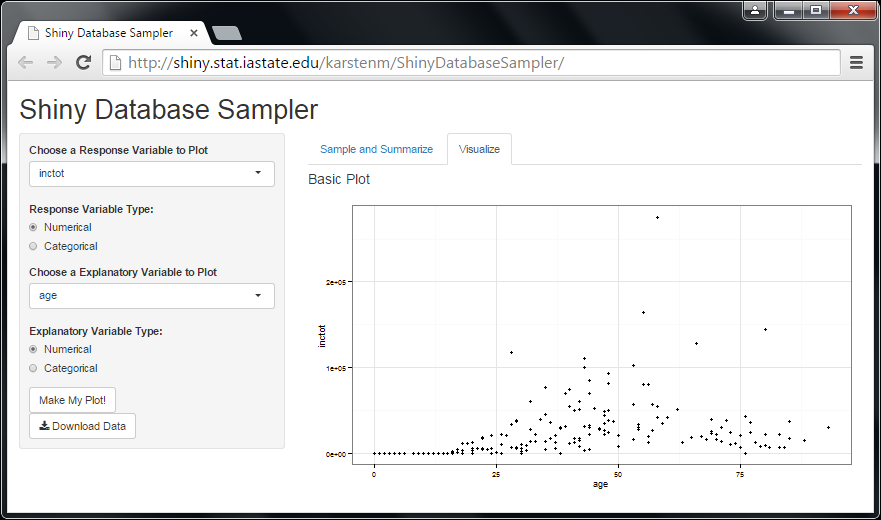
\includegraphics[keepaspectratio=TRUE,width=.99\textwidth]{ShinyDBSampler/Visualize.png}
\end{center}
\caption{Shiny Database Sampler Layout for \textit{Visualize} Tab} 
\label{fig:visualizetab}
\end{figure}

\begin{table}[hbtp]
\centering
\begin{tabular}{lll}
Response Variable & Explanatory Variable & Default Plot \\
\hline
Numerical & None & Histogram \\
Categorical & None & Barchart \\
Numerical & Numerical & Scatterplot \\
Categorical & Categorical & Stacked Barchart \\
Numerical & Categorical & Side-by-side Boxplots \\
\end{tabular}
\caption{Plot types supported in \textit{Visualize} tab.} 
\label{tab:defaultplottypes}
\end{table}

%%%-----------------------------------------------------------------------------------
\subsection{Applications}
\label{Applications}

The Shiny Database Sampler was developed for applications in statistics education and was implemented in the initial stages of development within the curriculum of an introductory statistics course. The alpha version of the software was used within one section of Statistics 104: \textit{Introduction to Statistics} for a group lab assignment and a course project. Later, a beta version was extended to be used in a lab assignment for six more sections of the same course. These two applications demonstrate possible uses of the Shiny Database Sampler. 

%-------------------------------------------------------------------------
 \subsubsection{Lab Application Overview} 
 \label{LabOverview}

The lab that utilized the Shiny Database Sampler was designed for students to think critically about sampling approaches, then the software allowed them to treat the large database as a population upon which to conduct their mock survey. Students were asked to consider the following pair of hypothetical situations:

\begin{enumerate}
\item Suppose that our goal is to estimate the mean age of all US residents. Similar to polling organizations we have a budget that allows us to survey around 1000 people. To collect our sample we decide to take a simple random sample of 1040 US residents.

\item Suppose now that our goal has changed.  Now we wish to investigate the association between age and state of residency. We want to compare the median ages for different states. We still have a budget that allows us to survey of 1040 people. To collect our sample we decide to take a stratified random sample of 20 residents from each state in the United States plus the District of Columbia and Puerto Rico. 
\end{enumerate}

In each scenario students were asked to discuss the choice of sampling scheme and to identify potential problems or difficulties. The students used the Shiny Database Sampler tool to obtain a sample from the database containing a 1\% microsample of the 2010 U.S. Census, from which they estimated mean and median age of U.S. residents. This lab was written to ensure that sampling concepts were the primary focus, with the Shiny Database Sampler acting in a supporting role. In order to avoid (sporadic) clicking of buttons to obtain samples without ever stopping to consider why the sampling approach matters, we intentionally designed the assignment to invite students to carefully consider sampling options {\it before} using the tool. The complete lab assignment can be found in Appendix \ref{labappend}. 


\subsubsection{Capstone Project Application Overview} 
\label{ProjectOverview} 

A second application of the Shiny Database Sampler was as an optional data source for a capstone project for students of Stat 104. Students were required to work in small groups to complete a capstone project that took a statistical approach to answering a question of their choosing. In order to accommodate students' interests in the subject matter of the project, groups were allowed to pick their own data source. The only specific requirement for the project was a written report that explained the collection of bivariate data and an analysis of the association -- included the appropriate plots, inference and interpretations to answer their question of interest.

Six of the groups chose to run a mock survey, using the databases available through the Shiny Database Sampler as a stand-in for a large population. These groups were required to demonstrate a strong argument for the sampling plan they used within the Shiny Database Sample. For instance, if a group wanted to know if the proportion of fatal accidents involving a drunk driver was higher in California than in Iowa; as part of the report they needed to argue why taking a stratified random sample of 100 fatal accidents per state would produce better information to answer their question than a simple random sample. Groups that gathered random samples from the Census and Accidents databases knew that they had gathered information from real life sources and they seemed genuinely engaged in the results of their projects. 
 
%%-----------------------------------------------------------------------------------
\subsection{User Survey for Software Evaluation}

As discussed above, the Shiny Database Sampler was designed for student use in course assignments. The quality of the software was initially assessed using a pluralistic walk through \citep{nielsen1994}, where the developer met iteratively with both statistical novices and experts to test the functionality of the early versions of the software. The software improvements that followed this inspection created the beta version of the Shiny Database Sampler that was ready for student use.

The second stage of evaluation for the Shiny Database Sampler was a user survey to learn student opinions about their experience from using the software during the lab assignment described above. Specifically, we are interested in three aspects of the software: we want to know if students find the tool easy to operate, if they see the connection to sampling concepts and if they find the data engaging. Exploring the student responses on these three topics of interest helps us to assess the quality of the Shiny Database Sampler as an educational software.

The ease of use of the Shiny Database Sampler is an considered an important attribute from both an educational psychology and a software development viewpoint. Cognitive load theory postulates that human capacity to process information is limited and that learning is composed of \textit{extraneous load}, effort to overcome obstructions to new knowledge, and \textit{germane load}, effort used to form new schema and integrate ideas with existing knowledge. \citet{muller2008} explain that ``Finding ways to increase germane load and minimize extraneous load has been a central pursuit of researchers under this paradigm." Application of cognitive load theory is extended to the setting of software in \textit{human centered design} \citep{oviatt2006}. The goal is to make interfaces for educational technologies intuitive and easy to operate in order to minimize the extraneous load; thus allowing more mental resources to be devoted to developing and integrating new knowledge. The intuitive construction of the user interface is an important component to software development, where the usability of a tool is defined by its learnability, understandability and operability \citep{manuel2002quality}.

Active learning requires a high cognitive load, and if prior knowledge is lacking more scaffolding is necessary to support learning \citep{muller2008}. Since sampling concepts are typically new for students, it is important that students clearly recognize sampling concepts in the interface; allowing it to be used as part of an assignment that is scaffolded for active learning. If students are able to identify the role of the Shiny Database Sampler as a tool for learning about random sampling, it is more easily integrated into the learning process.

Finally, assessing student engagement with the data sources in the Shiny Database Sampler is important because higher student engagement is linked to higher academic performance and learning \citep{carini2006student}. The GAISE guidelines recommend that technological tools should be used to help teach statistical concepts and that the use of real data is important for student engagement, hence we focus on these topics \citep{GAISEcollege}. \citet{Neumann2013} found that students consider real data more interesting and engaging. The hope is that students using the Shiny Database Sampler will find the real, nationally collected, governmental data sources engaging.

Student responses were collected in an anonymous survey following the group lab assignment -- as described in Section~\ref{LabOverview} -- that required students of an introductory statistics course, Stat 104, at Iowa State University to use the Shiny Database Sampler tool. Six sections of Stat 104 students were surveyed. The students were informed that the survey was not required and that no penalties or rewards were affiliated with its completion. Of the 320 students attending the lab, 265 completed the survey. 

%-------------------------------------------------------------------------
 \subsubsection{Survey Description} 

After completing the lab assignment, students were asked to respond to a survey consisting of twelve statements (referred to as \textit{items} in the following, see Table~\ref{tab:surveyquestions} for an overview). For each statement, students were asked for feedback on their level of agreement on a Likert scale from strongly disagree to strongly agree. 
The twelve items were designed to assess student opinion within three topics of four items each: ease of use, connection to sampling concepts, and engagement with the census data.  We will refer to these as the \textit{Ease}, \textit{Concept} and \textit{Engagement} item sets.  For each group of four items, two were worded positively and two were worded negatively. Introducing negation with half of the items was done to reduce the response bias associated with \textit{acquiescence} -- the tendency to respond positively irrespective of the item content due \citep{Furnham1986}. Responses were scored as -2 (strongly disagree), -1 (disagree), 0 (neutral), 1 (agree), 2 (strongly agree).  Responses for negatively worded items were reverse-scored for the purposes of analysis.

\begin{table}[hbtp]
\centering
\small
% \scalebox{0.9}{
\begin{tabular}{ccp{3.4in}crr}
Topic Set & ID & Item & Polarity & Mean & SD\\[3pt]
  \hline
Ease & 1 & \it I found the web tool easy to use & $+$ & 0.84 & 0.76\\  
 & 2 & \it The layout of the web tool was intuitive & $+$  & 0.63 & 0.74\\  
 & 3 & \it Using the web tool was difficult & $-$  & 0.77& 0.88\\  
 & 4 & \it Learning to use the web tool was hard & $-$  & 0.81 & 0.85\\  [3pt]
  \hline
Concept & 1 & \it The web tool helped me understand sampling concepts & $+$  & 0.80& 0.78\\   
& 2 & \it I understand sampling ideas less after using the web tool & $-$  & 0.83& 1.01\\  
& 3 & \it Sampling techniques are clearer after using the web tool & $+$  & 0.58& 0.73\\  
& 4 & \it The web tool made me less sure how to randomly sample & $-$  & 0.89& 0.87\\  
   \hline
Engagement & 1 & \it I did not enjoy working with the Census data & $-$  & 0.38 & 1.01\\  
& 2 & \it I thought the Census data was boring & $-$   & 0.23& 0.97\\  
& 3 & \it Knowing that the Census data was from real people made it more interesting & $+$  & 0.82& 0.84\\   
& 4 & \it I liked analyzing the Census data & $+$  & 0.28 & 0.86\\   
\end{tabular}
% }
\caption{Survey questions and response summaries for all items \textit{after} Reverse-Scoring (RS)}
\label{tab:surveyquestions}
\end{table}

\normalsize

From Table~\ref{tab:surveyquestions} we see that all response averages are positive after reverse-scoring. With the Ease items this indicates that students tend to find the tool relatively easy to operate. For frame of reference, we assume that students are comparing the difficulty of use with other educational technologies and webpages they have encountered in the past; in particular the \texttt{JMP} software used previously on their Stat 104 labs and homework. Students also tend to respond to Concept items in a manner that is affirmative that the tool connects them to sampling concepts. Students' responses are near to neutral for most items about engagement with the census data, with the exception of Engagement item 3.  The phrasing of this question seems to have led students to reconsider their engagement level and led to a consistently more positive attitude.

%-------------------------------------------------------------------------
\subsubsection{Assessment of Internal Consistency for Item Topic Sets} 

The goal for this survey is to use the responses to sets of items to infer student opinions about the underlying topic of each set.  It is reasonable to aggregate the responses over entire questions sets if we can show that items within each set are measuring the same latent topic. We use fluctuation diagrams and Cronbach's $\alpha$ \citep{cronbach:51} to assess this internal consistency. 

A fluctuation diagram is the visual analog of the contingency table, displaying frequency of each unique responses combination as the area of blocks on the bivariate grid containing all possible pairs of response values. A fluctuation diagram with large blocks on the diagonal indicates strong agreement or {\it internal consistency} between responses of the two items.  Figure~\ref{fig:fluctuationDiagrams} contains fluctuation diagrams for all item pairs within topic sets.    
We notice that most pairs of responses fall heavily along the diagonal and are primarily in the upper right of each diagram. This indicates that most items within sets have strong agreement and that the response values are generally neutral to positive for all items (after reverse-scoring the negative statements).
For the item pairs in the Concept topic set we see that fluctuation diagrams have slightly larger off-diagonal trends than items within the other two sets, which indicates a lower level of internal consistency for Concept items than in the other two topic sets. 

\begin{knitrout}
\definecolor{shadecolor}{rgb}{0.969, 0.969, 0.969}\color{fgcolor}\begin{figure}[hbt]

{\centering \includegraphics[width=.98\linewidth]{FigurefluctuationDiagrams-1} 

}

\caption[Fluctuation Diagrams of All Item Pairs within Topic Sets]{Fluctuation Diagrams of All Item Pairs within Topic Sets}\label{fig:fluctuationDiagrams}
\end{figure}


\end{knitrout}



Cronbach's $\alpha$ measures internal consistency within an item set by comparing the sum of individual response variances to the variance of the sum of the responses. It is defined as follows
%
\begin{equation} \label{eq:alpha}
\alpha = K/(K-1) \cdot \left(1 - \left . \sum_{i=1}^K \V{Y_i} \right /  \V{\sum_{j=1}^K Y_j}\right),
\end{equation}
%
where $Y_i$ denotes the response on the $i^{\text{th}}$ survey item ($ i = 1,... , K$), and $K$ is the number of survey items considered for internal consistency. Generally, $K=4$ for the item sets of this survey.
Cronbach's $\alpha$ reaches a maximal value of 1, if there is perfect agreement between items (i.e. all responses to the same item set are identical). In the case that items sets are independent, the internal consistency is measured as $\alpha = 0 $. Cronbach's $\alpha$ can be negative in the situation of consistent \textit{disagreement} between responses and will approach negative infinity if there is perfect disagreement between items.  See appendix~\ref{appendCronbach} for details on the bounds for Cronbach's $\alpha$. 

\citet{Nunnally1978} propose that a Cronbach's $\alpha$ of 0.7 or above should be considered as an indication of ``modest reliability''.   \citet{GeorgeMallery2003} provide the commonly used extended scale, displayed in Table~\ref{GMAlphaScale}, for interpreting internal consistency based on Cronbach's $\alpha$. \\

\begin{table}[hbtp]
\centering
\begin{tabular}{ll}
\hline 
Internal Consistency & Range \\
\hline
Excellent &  $[ 0.9 , 1.0 ]$ \\
Good & $[ 0.8 , 0.9 )$ \\
Acceptable & $[ 0.7 , 0.8 ) $\\
Questionable & $[ 0.6 , 0.7 )$ \\
Poor & $[ 0.5 , 0.6 )$ \\
Unacceptable & $( -\infty, 0.5 )$ \\
\hline
\end{tabular}
\caption{Extended Scale for Cronbach's $\alpha$  (George and Mallery, 2003).} 
\label{GMAlphaScale}
\end{table}

Since Cronbach's $\alpha$ is a sample estimate for the internal consistency of an item set, it experiences sampling variability. Under the assumption of normally distributed responses, Cronbach's $\alpha$ follows approximately an $F_{\nu_1,\nu_2}$, where $\nu_1 = n-1$ and $\nu_2$ is based on a function of the eigenvalues from the quadratic linear combination of the roots of the variance matrix \citep{KistnerMuller2004}. Assuming normality to construct confidence intervals for the true internal consistency of item sets would be questionable for the responses in this survey, so we have elected to bootstrap the intervals instead.

Table~\ref{cronbachstuff} displays the point estimates and 95\% central bootstrap intervals for Cronbach's $\alpha$ for each item set from the student survey.  The intervals were created using quantiles of the Cronbach's $\alpha$ values from 10,000 bootstrap resamples. 
 The results indicate modest levels of internal consistency for Ease and Engagement item sets, and a lower level for the Concept item set. This is in agreement with the findings based on the fluctuation diagrams in Figure~\ref{fig:fluctuationDiagrams}. 



% latex table generated in R 3.0.2 by xtable 1.7-3 package
% Tue Nov 04 15:05:46 2014
\begin{table}[hbtp]
\centering
\begin{tabular}{lrc}
  \hline
Set & Estimate & 95\% Confidence Interval \\ 
  \hline
Ease & 0.70 & (0.613 , 0.759)\\ 
  Concept & 0.53 & (0.410 , 0.637) \\ 
  Engagement & 0.72 & (0.643 , 0.776) \\ 
   \hline
\end{tabular}
\caption{Cronbach's $\alpha$ Estimates for each item set with 95\% central bootstrap confidence interval based on 10,000 bootstrap samples} 
\label{cronbachstuff}
\end{table}

\subsubsection{Assessment of Polarity Issues}  

We next turn our attention to the polarity of the survey items; specifically we consider that positive and reverse-scored negative items may elicit a different responses. The survey contained six unique item pairs based on topic and polarity combinations. Figure~\ref{fig:OverallSetBars} compares the distribution of responses from positive and negative item pairs within topics.  We see strong similarity between positive and reverse-scored negative items in response distributions for the Ease and Engagement item sets. The Concept item set however displays a noticeable difference in response distributions from each polarity.  In particular, we see that students are more neutral toward the positively worded questions. This polarity difference in student responses explains the lower internal consistency measured by Cronbach's $\alpha$, and may be partly due to the problem that the negation of positive constructs can be linguistically counter-intuitive \citep{Friborg2006}. For instance, students may interpret the statement ``It is not less clear'' differently than the statement ``It is more clear''.

\begin{knitrout}
\definecolor{shadecolor}{rgb}{0.969, 0.969, 0.969}\color{fgcolor}\begin{figure}[hbt]

{\centering \includegraphics[width=.99\linewidth]{FigureOverallSetBars-1} 

}

\caption[Item set response distributions]{Item set response distributions}\label{fig:OverallSetBars}
\end{figure}


\end{knitrout}


To assess whether responses from positive and reverse-scored negative items can be reasonably grouped together within topic sets we turn to principal component analysis.  We first combine the item pairs into averages for each of the six topic and polarity combinations, then we decompose these six scores into principal components. The component variances and factor loadings from this decomposition are found in Table~\ref{pc6table}. We argue that the data could be reasonably reduced to four principal components because each of these components explains over 10\% of the variance and together they explain 87.4\% of the total variation.  The uniformly aligned factor loadings for Component 1 reflect the general tendency toward student agreement to all items on the survey.  The factor loadings for Components 2 and 3 displayed in Figure~\ref{fig:PCA6plot} show similar projections for positive and negative item scores for Ease and Engagement pairs but a dramatic separation in the positive and negative item scores for the Concept set.  \\  



\begin{table}[hbtp]
\centering
\begin{tabular}{lrrrrrrr}
\hline 
& Principal Component & 1 & 2 & 3 & 4 & 5 & 6 \\ 
\hline
Variances \hspace{.1in} & Prop. of Var & 0.457 & 0.181  & 0.135 & 0.101 & 0.071 & 0.055  \\
& Cumu. Prop. of Var & 0.457 & 0.638  & 0.773 & 0.874 & 0.945 & 1.000  \\
\hline
Loadings & Pos. Ease & -0.292 & 0.169 & -0.509 & -0.036 & -0.055 & 0.789\\
& Neg. Ease &  -0.444 & -0.390 & -0.464 & 0.429 & 0.372 & -0.335\\
& Pos. Concept &  -0.304 & 0.330 & -0.389 & -0.350 & -0.537 & -0.487\\
& Neg. Concept &  -0.408 & -0.641 & 0.250 & -0.585 & -0.067 & 0.116\\
& Pos. Engaged &  -0.367 & 0.523 & 0.207 & -0.321 & 0.663 & -0.083\\
& Neg. Engaged &  -0.569 & 0.164 & 0.519 & 0.496 & -0.355 & 0.087\\
\hline
\end{tabular}
\caption{Summary Statistics from Principal Component Analysis with Six Topic/Polarity Item Pairs} 
\label{pc6table}
\end{table}

\begin{knitrout}
\definecolor{shadecolor}{rgb}{0.969, 0.969, 0.969}\color{fgcolor}\begin{figure}[hbt]

{\centering \includegraphics[width=.5\linewidth]{FigurePCA6plot-1} 

}

\caption[Item Pair Loadings on Components 2 and 3 from the Principal Component Analysis with Six Topic/Polarity Item Pairs]{Item Pair Loadings on Components 2 and 3 from the Principal Component Analysis with Six Topic/Polarity Item Pairs}\label{fig:PCA6plot}
\end{figure}


\end{knitrout}

This principal component analysis, with all topic and polarity combinations, suggests that we can reduce the dimensionality by combining the positive items with the reverse-scored negative items for Ease and Engagement topics.  This leaves only the Concept item set separated based on polarity for final analysis.  The decision to combine the responses for Ease and Engagement items also aligns with the higher internal consistency for these item sets as displayed in Cronbach's $\alpha$ values and fluctuation diagrams in Figure~\ref{fig:fluctuationDiagrams}. Thus, we will carry forward with the final analysis using four resulting item sets: Ease, Positive Concept, Negative Concept and Engagement. 

\subsubsection{Assessment of Orthogonality} 

The next major consideration is whether the item sets are truly measuring different latent topics, and therefore can be view as non-redundant. The ability of the survey to separately measure the topics of Ease, Concepts and Engagement can be assessed through the orthogonality of the responses from different item sets. To check the orthogonality of the sets we conduct another principal component analysis; this time on the average responses for each student from the four item sets -- Ease, Positive Concept, Negative Concept and Engagement.  Items sets will be considered highly orthogonal if the principle component analysis cannot reduce the dimensionality from the four sets. 



\begin{table}[hbtp]
\centering
\begin{tabular}{lrrrrr}
\hline 
& Principal Component & 1 & 2 & 3 & 4 \\ 
\hline
Variances \hspace{.1in} & Prop. of Var & 0.515 & 0.249  & 0.134 & 0.102  \\
& Cumu. Prop. of Var & 0.515 & 0.764  & 0.898 & 1.000  \\
\hline
Loadings & Ease & -0.430 & 0.144 & -0.307 & 0.837\\
& Pos. Concept &  -0.408 & 0.562 & -0.520 & -0.497\\
& Neg. Concept &  -0.619 & -0.745 & -0.101 & -0.227\\
& Engagement &  -0.515 & 0.330 & 0.790 & -0.031\\
\hline
\end{tabular}
\caption{Principal Component Analysis with Final Four Item Sets} 
\label{pctable}
\end{table}

Table~\ref{pctable} displays the proportion of variance explained by each of the four principal components and factor loadings. The first principal component has similar loadings from all item sets, which we can interpret as the general tendency toward positively scored responses on all items. The second, third and fourth principal components create separation for mean responses of the Negative Concept item set, the Engagement item set and the Ease item sets, respectively. The variances in Table \ref{pctable} reveal that over 10\% of the variation is explained by the fourth component, thus it is necessary to retain all four principal components. This inability to reduce dimensionality implies that average student responses from the four item sets are largely orthogonal. Based on the separation in the loadings and the orthogonality of the principal components, we conclude that the average response scores from the four item set have interpretability as measurements of unique latent topics. 


%-------------------------------------------------------------------------
\subsubsection{Survey Assessment Results} 

In the analysis of student responses, we find that the internal consistency, assessed with Cronbach's $\alpha$ and fluctuation diagrams, is acceptable for interpreting the combined item responses that measure ease of use and engagement with the census data. We do not have the same certainty with the responses to Concept items and therefore split the Concept items into two sets: the Positive and Negative Concept item sets. This split is supported by the initial principal component analysis of the six topic and polarity item pair scores. The follow-up principal component analysis on the combined responses for each of the four resulting item sets indicates that the factors were all fairly orthogonal. This ensures us that the survey was effective at eliciting unique characteristics of the user experience.

The barcharts found in Figure \ref{fig:OverallSetBars} show that the distribution for each item set is heavily skewed to the left, with the majority of students having neutral to positive responses. The small tail to the left in each distribution indicates that there was a small minority of students with expressedly negative views. The response distributions indicate that on average students found the Shiny Database Sampler easy to use, found that the tool connected them to sampling concepts and felt moderately engaged with the census data that was accessed with the application. 


\section{Conclusions and Future Work}

The Shiny Database Sampler allows point-and-click access to large databases through the mechanism of random sampling. This approach adds pedagogical value over the use of static samples because it allows for course activities to highlight the concepts and process of collecting data through random sampling. The lab and project application of the Shiny Database Sampler within an introductory course were designed to emphasize thought about sampling concepts and the data, not about the software. Toward this scaffolded approach, the design aimed to make the interface easy to use, clearly display sampling concepts and provide engaging data. The student user survey indicates that these goals were met.

The Shiny Database Sampler could naturally be updated to access additional databases or provide more statistical analysis or visualization options directly within the interface. Also in future work, a similar interface could be developed where the user specifies an aggregation scheme instead of a sampling scheme. This approach would be more true to exploration techniques of big data sources than using random sampling; this would be a distinct -- and perhaps exciting -- departure from the content of a traditional introductory statistics curriculum. In such an interface, grouping variables or binning parameters could be used to direct dynamic data aggregation to then be explored; using display such as histograms or binned scatterplots. As the size and ubiquity of data in the world grows, students would be well served by attempts to thoughtfully incorporate big data into the undergraduate statistics curricula.

% %-------------------------------------------------------
% \appendix (MOVED TO Appendix1.Rnw File)
% %-------------------------------------------------------
% \section{Appendix: Lab Assignment}
% \label{labappend}
% 
% For this activity you will be using a tool called the Shiny Database Sampler to take a random sample of United States residents from US census data. The census data is the Public Use Microdata Sample (PUMS) which is a 3 million person subset of the entire Census data.  For this activity we treat our samples as though they are selected from the full census records.  \\ 
% 	
% We are going to explore how these random sampling plans relate to the goals of a sample survey. The tool will allow you to define either a simple random sampling plan or a stratified random sampling plan. In the following two scenarios we will explore the advantages and disadvantages of these two sampling plans. Access the tool at \url{http://shiny.stat.iastate.edu/karstenm/ShinyDatabaseSampler}. \\	 
% 
% \underline{Scenario 1:} Suppose that our goal is to estimate the mean age of all US residents. Similar to polling organizations we have a budget that allows us to survey around 1000 people. To collect our sample we decide to take a simple random sample of 1040 US residents. \\
% 
% \begin{enumerate}[(a)]
% \item Is this study and example of an experiment or an observational study?  Explain your answer.
% \item	Your colleague Bob claims that we are wasting our budget to get only 1040 people using random sampling. He says that we could get 20000 responses to the survey if we invested that money into a mailing campaign in Minneapolis. Explain why the random selection is important.
% \item	Another colleague, Jill, asks why we do not stratify by state when we take the sample so that we get 20 people from each of the 50 states along with Puerto Rico and the District of Columbia. Explain why this idea would not create a representative sample to pursue our goal.
% \end{enumerate}
% 
% Now that we have decided on our sampling plan, let's go collect our data.  The Shiny Database Sampler needs to be told 4 pieces of information in order to collect census records the way you want. (1) Choose the database called ``Census'', (2) select the ``simple random sample'' option, (3) enter a random seed, any number between 1 and 10000, you can do this by rolling a 10-sided die 4 times and (4) lastly tell it that we want ``1040'' random draws. Once you have drawn your samples the page will display basic summary statistics for the variables in the census.\\
% 
% \begin{enumerate}[(a)]
% \setcounter{enumi}{3}
% \item Report the 5-number summary and sample mean age.
% \item	Use the 5-number summary to construct a box plot of age.
% \item	Go to the ``Visualize'' tab.  Choose age as your Response Variable to Plot.  What type of variable is this?  By clicking on Make My Plot? a histogram of the sample of ages will be displayed.  Describe the shape of the data distribution of age.
% \item	Is the relationship between the sample mean and sample median consistent with your description of shape?  Explain briefly.
% \item	If our goal was to not only estimate the mean age of all the U.S. residents but also come up with estimates of the median age of all residents in each of the 50 states, plus the District of Columbia and Puerto Rico what is a drawback of using the simple random sample of 1040?  Hint: Set the Data Table to display 100 records per page and go to the page that has ``states'' 10 and 11 (Delaware and the District of Columbia).
% \end{enumerate}
% 
% \underline{Scenario 2:} Suppose now that our goal has changed.  Now we wish to investigate the association between age and state of residency. We want to compare the median ages for different states. We still have a budget that allows us to survey around 1040 people. To collect our sample we decide to take a stratified random sample of 20 residents from each state in the United States plus the District of Columbia and Puerto Rico. 
% 
% \begin{enumerate}[(a)]
% \setcounter{enumi}{8}
% \item  Explain in general why collecting a stratified random sample is a better plan than a simple random sample for answering this question.  
% \end{enumerate}
% 
% Now that we have decided on our new sampling plan, let's go collect our data.  The Shiny Database Sampler will need to be told 5 pieces of information in order to collect census records the way you want this time. (1) Choose the database called ``Census'', (2) select the ``stratified random sample'' option, (3) enter a random seed, any number between 1 and 10000, you can do this by rolling a 10-sided die 4 times, (4) select ``state'' as strata variable and (5) lastly tell it that we want ``20'' random draws from each state, plus the District of Columbia and Puerto Rico.  \\
% 
% It will take a minute or two to collect these data. It is sifting through millions of records and randomly selecting them from within state groups after all! Once you have drawn your samples you can take a peek at your data set in the main panel of the webpage. You will be able to answer the following questions using the summaries provided on the webpage.  \\
% 
% You will notice that the summaries are all broken down by state, but the states are not given names, they are given a code number.  This is done on the census to save computer storage space (saving a ``19'' is much smaller than ``Iowa'').  A list of all the state codes is available at \url{https://www.census.gov/geo/reference/ansi\_statetables.html} (Click on FIPS Codes for the States and the District of Columbia).\\ 
% 
% 
% 
% \begin{enumerate}[(a)]
% \setcounter{enumi}{9}
% \item Report the mean and 5-number summary for the age of the sample from the state of Iowa (\texttt{state = 19}).
% \item	Report the mean and 5-number summary for the age of the sample from the state of Alaska (\texttt{state = 2}).
% \item	Compare the distribution of ages in Alaska and Iowa using the values from parts j and k.
% \item	Making comparisons as we have done above would become tedious if we wanted to compare ages between all pairs of states in the country.  What would be a good way to visually display this information so aid in making these comparisons? Explain your answer.
% \end{enumerate}
% 
% 
% % %------------------------------------------------------------------
% % \section{Appendix: Technical Implementation of Shiny Application}
% % \label{appendConstruction}
% % 
% % \textbf{Construction schematics and description of sampling process and plotting process.}
% % 
% % 
% % %------------------------------------------------------------------
% % \section{Appendix: Database Descriptions}
% % \label{appendDB}
% % 
% % \textbf{To be detailed when databases updated and origins better known.}
% 
% %------------------------------------------------------------------
% \section{Appendix: Cronbach's $\alpha$ Properties}
% \label{appendCronbach}
% 
% Recall the form of Cronbach's $\alpha$ from equation~(\ref{eq:alpha}):
% 
% \begin{center}
% $\alpha = \left(K/(K-1)\right) \left( 1- \sum_{i=1}^K \V{Y_i} \right.\left/  \V{\sum_{j=1}^K Y_j}  \right)$,
% \end{center}
% 
% \textit{Claim 1:} Perfect agreement in items leads to $\alpha = 1$ 
% 
% \textit{Proof:} Let $ Y = Y_1 = Y_2 = ... = Y_k$, thus having perfect agreement.
% 
% $\Rightarrow$  $\text{Cov}(Y_i, Y_j) = \V{Y} = \sigma^2_y $ \hspace{.1in} $\forall i\ne j$ \\
% 
% $\Rightarrow$  $\V{\sum_{j=1}^K Y_j }$ = $\sum_{i=1}^K \V{Y_i} + \sum_{i\ne j}\text{Cov}(Y_i, Y_j)$ =  $K\sigma^2_y + K(K-1)\sigma^2_y$ \\
% 
% $\Rightarrow$  $\alpha = \left(K/(K-1)\right) \left( 1- \sum_{i=1}^K \V{Y_i} \right.\left/  \V{\sum_{j=1}^K Y_j}  \right)$ = \\
% \indent \hspace{.2in} $\left(K/(K-1)\right) \left( 1- K\sigma^2_y \right.\left/ K\sigma^2_y + K(K-1)\sigma^2_y \right)$ =\\
% \indent \hspace{.2in} $\left(K/(K-1)\right)  (1- 1/K)$ = $\left(K/(K-1)\right) ((K-1)/K)$ = $1$ \\
% 
% \vspace{.25in} %------------------------------
% 
% \textit{Claim 2:} For independent items $\alpha = 0$ 
% 
% \textit{Proof:} Let $Y_1 = Y_2 = ... = Y_k$ be independent 
% 
% $\Rightarrow$ $\sum_{i=1}^K \V{Y_i} = \V{\sum_{j=1}^K Y_j} $ 
% 
% $\Rightarrow$  $\alpha = \left(K/(K-1)\right) \left( 1- \sum_{i=1}^K \V{Y_i} \right.\left/  \V{\sum_{j=1}^K Y_j}  \right)$ = \\
% \indent \hspace{.2in} $\alpha = \left(K/(K-1)\right) \left( 1- \V{\sum_{j=1}^K Y_j} \right.\left/  \V{\sum_{j=1}^K Y_j}  \right)$ = \\
% \indent \hspace{.2in} $\alpha = \left(K/(K-1)\right) \left( 1- 1 \right)$ = 0 
% 
% \vspace{.25in} %------------------------------
% 
% \textit{Claim 3:} Perfect disagreement in items leads to $\alpha = -\infty$ 
% 
% \textit{Proof:} Let $K=2$ and $Y_1 = -Y_2$, thus having perfect disagreement.
% 
% $\Rightarrow$  $\V{Y_1 + Y_2}$ = $\V{Y_1 - Y_1}$ = $\V{0}$ = $0$
% 
% $\Rightarrow$  $\alpha = \left(K/(K-1)\right) \left( 1- \sum_{i=1}^K \V{Y_i} \right.\left/  \V{\sum_{j=1}^K Y_j}  \right)$ = $(2/1)(1-2\sigma^2_y/0)$ = $-\infty$ 
\chaptocbreak

\chapter{BINNING STRATEGIES AND RELATED LOSS FOR BINNED SCATTERPLOTS}
\label{BinnedScatter}


%opening
% \title{Binning Strategies and Related Loss for Large Data Visualization}
% \author{Karsten Maurer$^1$, Susan VanderPlas$^1$, Heike Hofmann$^{1,2}$\\$^1$Department of Statistics, $^2$Human Computer Interaction\\Iowa State University}
 
\begin{center}
\textbf{Status}: In Preparation for Submission to \textit{Journal of Computational and Graphical Statistics} (JCGS)\\
\end{center} 

\begin{center}
\textbf{Authors}\\
Karsten Maurer, Iowa State University, Primary Author\\
Heike Hofmann, Iowa State University\\
Susan Vanderplas, Iowa State University\\
\end{center}

\begin{center}
\textbf{Abstract}\\
\end{center}

Dealing with the data deluge of the Big Data Age is both exciting and challenging. The demands of large data require us to re-think strategies of visualizing data. Plots employing binning methods have been suggested in the past as viable alternative to standard plots based on raw data, as the resulting area plots tend to be less affected by increases in data. This comes with the price of the loss of information inherent to any binning scheme. In this paper we discuss binning algorithms used in the construction of binned scatterplots. We define functions to quantify the loss of spatial and frequency information and discuss the effects of binning specification on loss in the framework of simulation and case studies. From this we provide several practical suggestions for binning strategies that lead to binned scatterplots with desirable visual properties. 

\section{Introduction}
\label{Intro}





Technological advances have facilitated collection and dissemination of large data as records are digitized and our lives are increasingly lived online. According to an EMC report in 2014 ``the digital universe is doubling in size every two years and will multiply 10-fold between 2013 and 2020 - from 4.4 trillion gigabytes to 44 trillion gigabytes" (\url{http://www.emc.com/about/news/press/2014/20140409-01.htm}). This ``Data Deluge" of the Big Data Age (NY Times, Feb 2012) poses exciting challenges to data scientists everywhere: ``It's a revolution $\dots$ The march of quantification, made possible by enormous new sources of data, will sweep through academia, business and government. There is no area that is going to be untouched"-- Gary King, Harvard Institute.  
 
Data sets with millions of records and thousands of variables are not uncommon. \citet{Friedman97} proposed in his paper on data mining and statistics that ``Every time the amount of data increases by a factor of ten, we should totally rethink how we analyze it". \citet{jacobs2009} echoed the sentiment, stating that ``big data should be defined at any point in time as \textit{data whose size forces us to look beyond the tried-and-true methods that are prevalent at that time}". The same holds true for visualizations. With a 100-1000 fold increase in the amount of data, the utility of some of our most commonly used graphical tools, such as scatterplots, deteriorates quickly \citep{gold}. 

Area plots, such as histograms, do not tend to be as affected by increases in the amount of data because they display aggregations instead of raw data. By using binning strategies and the principles for displaying information in area plots, scatterplots can again become useful instruments for large data settings \citep{gold}.

In this paper we describe first the inadequacy of traditional scatterplots in large-data situations. We discuss different binning algorithms use in the construction of binned scatterplots and the \textit{loss of information} inherent to binning. We will then explore the effects of binning specification on the properties of binned scatterplots through simulation and real-data case studies. We conclude with several practical suggestions for binning specifications for creating binned scatterplots that have desirable visual properties. 

\section{Scatterplots for Large Data Sets}
\label{Scatter}

In the case of modestly sized data, scatterplots are great tools for showing bivariate data relationships. With large data, scatterplots suffer from over-plotting of points, which masks relevant structure. Figure~\ref{fig:scatter-alpha} shows an example taken from baseball statistics. The scatterplot shows 139 seasons (from the years of 1871 -- 2009) of  pitching statistics for every baseball pitcher as published in Sean Lahman's Baseball database (\url{http://www.seanlahman.com/baseball-archive/}).  The number of games played in a season is plotted against the number of strikeouts a pitcher threw over the course of a season. While the data set is only medium sized with 42583 observations, it already shows some of the break-down patterns scatterplots experience with large data. 

Figure~\ref{fig:scatter-alpha}(a) shows a traditional scatterplot with each observation is drawn with a filled circle. A triangular structure is apparent with some outliers at a medium number of games and high number of strikeouts; however the density within the triangular mass of points is indistinguishable. \citet{tukey} suggested the use of open circles (see Figure~\ref{fig:scatter-alpha}(b)) to mitigate the problem of over-plotting. Open circles make points that are close together more visually distinct; thus allowing for the perception of more density information than with filled points.  A modern alternative to open circles is alpha blending (see Figure~\ref{fig:scatter-alpha}(c)). Alpha blending renders points as semi-transparent to provides more visibility of underlying points.

\begin{figure}[hbtp]
  \subfloat[Overplotted data ]{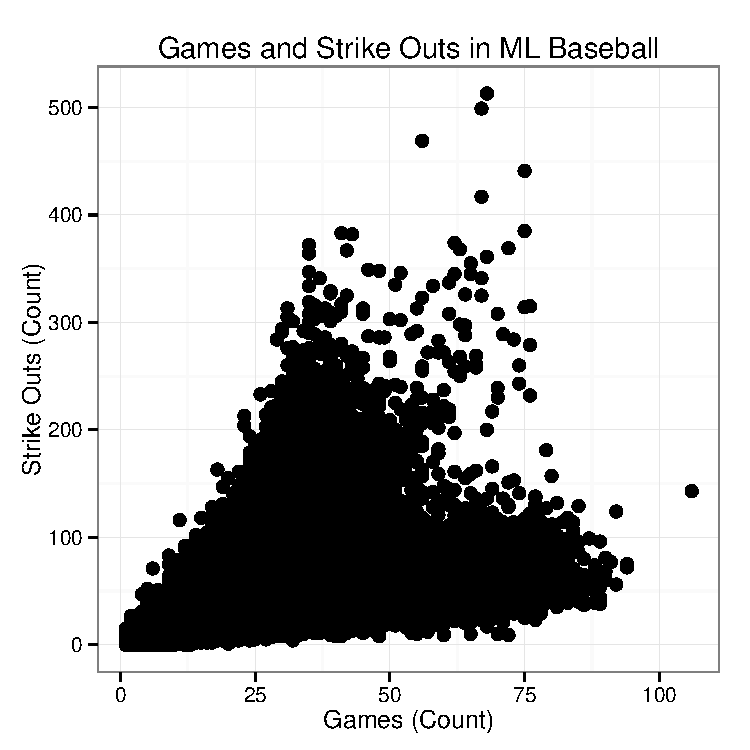
\includegraphics[keepaspectratio=TRUE,width=.31\textwidth]{./Body/BinnedScatter/figure/Overplotting.pdf}}
  \subfloat[Tukey-style open circles]{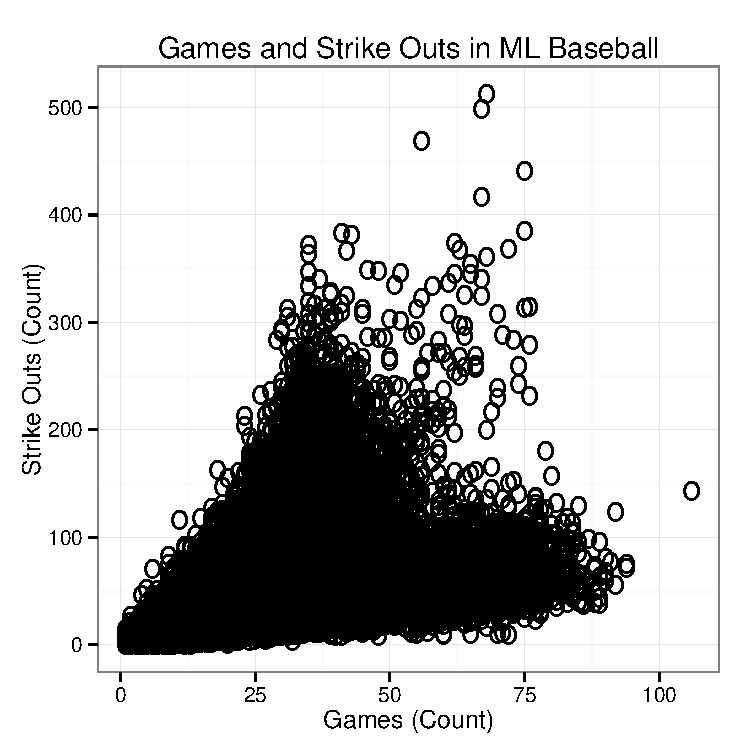
\includegraphics[keepaspectratio=TRUE,width=.31\textwidth]{./Body/BinnedScatter/figure/OverplottingCircles.pdf}} 
	\subfloat[Alpha blending]{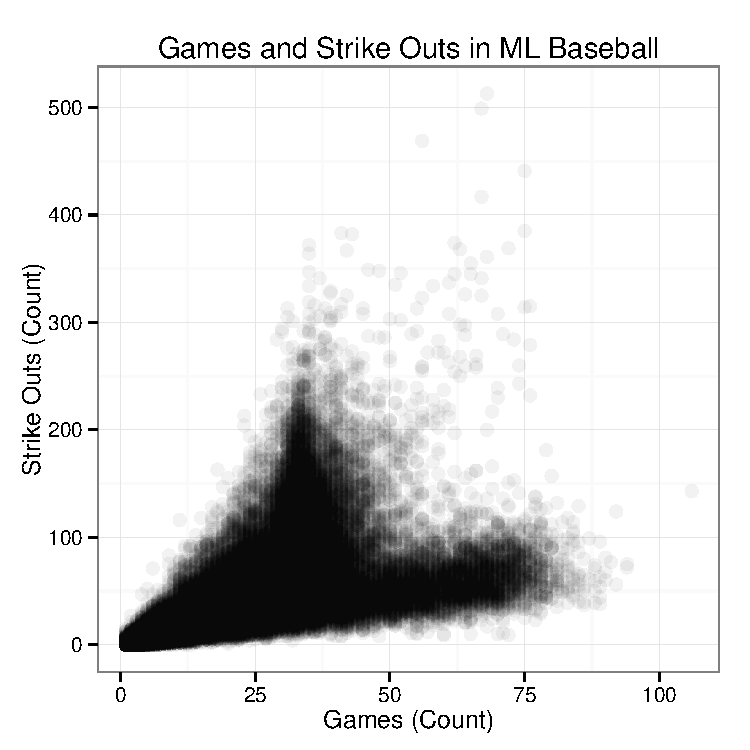
\includegraphics[keepaspectratio=TRUE,width=.31\textwidth]{./Body/BinnedScatter/figure/OverplottingAlpha.pdf}}
  
  \subfloat[Hexagonal binned scatterplot]{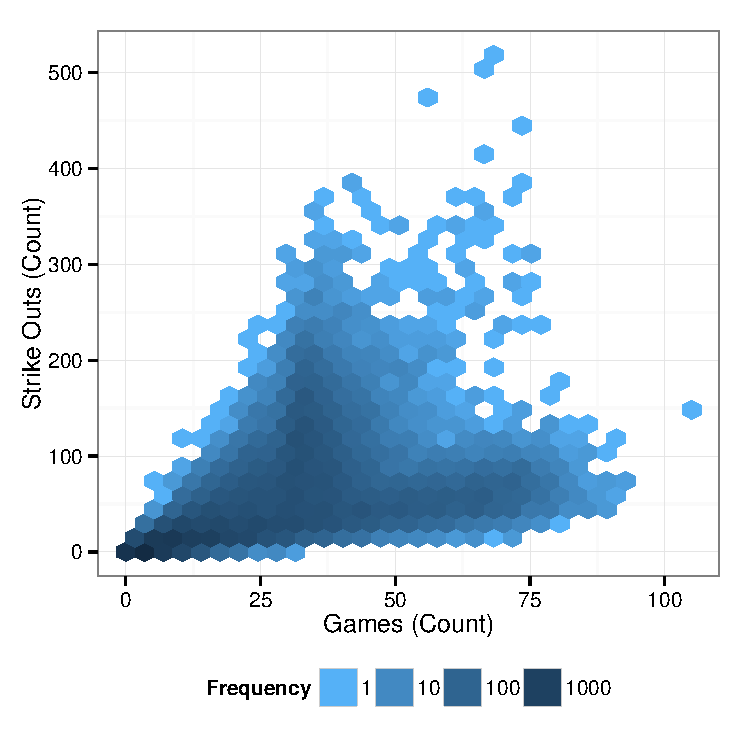
\includegraphics[keepaspectratio=TRUE,width=.48\textwidth]{./Body/BinnedScatter/figure/HexBinning.pdf}}
  \subfloat[Hexagonal binned bubble plot]{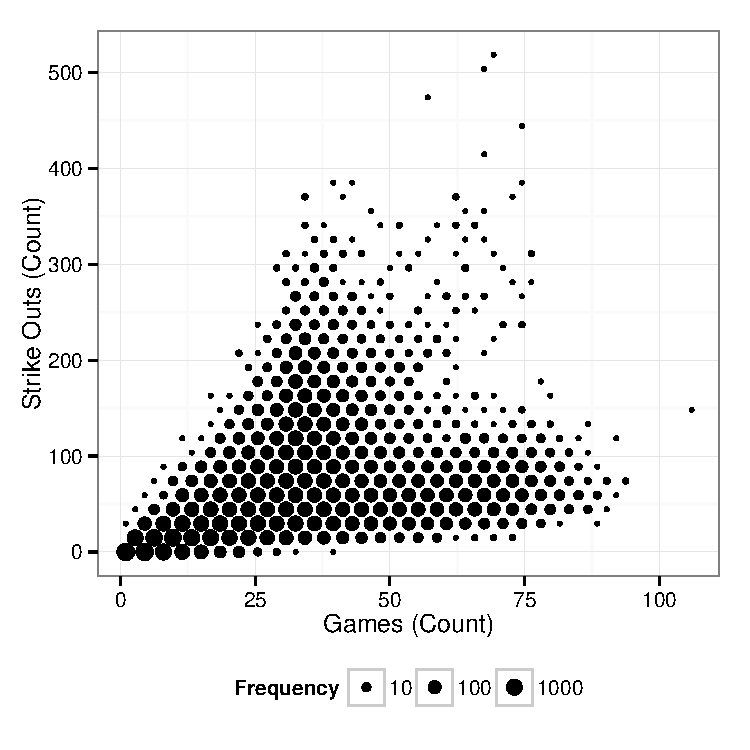
\includegraphics[keepaspectratio=TRUE,width=.48\textwidth]{./Body/BinnedScatter/figure/BinScatter.pdf}} 

	\caption{\label{fig:scatter-alpha} Scatterplots of Games versus Strikeouts in Major League Baseball, using different strategies of dealing with the issue of over-plotting:  (a) uses standard, opaque, filled circles, (b)  uses Tukey's recommended open circles, and (c) uses filled circles with alpha blending ($\alpha$=0.05). Plots (d) and (e) show hexagonal binning strategies with frequency mapped to color and area respectively}
\end{figure}

All of these methods fall short in the example.
As can be seen in Figure~\ref{fig:scatter-alpha}, strategy (a) is the least effective, as it provides information about the outliers and range of the data but cannot provide any point density information. Tukey's open circles (b) help to a degree, but are also prone to over-plotting  when the data set is very large. Alpha blending (c) highlights the structure, but minimizes the visual impact of outliers. The data set is large enough that neither alpha blending nor open circles are completely effective, and so we must pursue a different strategy which can provide better information about the relative density of points at a given location.

Other scatterplot adaptations have been introduced that avoid over-plotting by manipulating the display of the points by distorting the locations or the scales. Generalized scatterplots \citep{Keim2010GenScatter} display all individual observations, including those sharing identical coordinates, and use distortion of the point locations by having points repel one another to avoid overlapping. An extension of generalized scatterplots uses clustering and local principal components to allow ellipsoid oriented distortion to display local correlation structure in the data \citep{Janetzko2013Ellipse}. Variable-binned scatterplots \citep{Hao2010visual} break the display into a non-uniform rectangular grid and resize the rows of cells according to density of points. This variable binning fragments the continuity of the axes into segments on different scales and also does not deal with points at identical coordinates. Generalized and variable-binned scatterplots make fine data structure more visible and allow color to be reserved for a third variable instead of frequency; however, the distortion of the point locations and/or axes warp the visual display of the association between the two primary variables.

Another approach is to reduce the graphical complexity by plotting binned aggregations of the data, namely frequencies, as opposed to plotting every observation as an individual point. This has the additional advantage of reducing the size of the stored data necessary for the construction of the plot, as only the bin centers and the bin frequencies must be stored. Wickham argues for a ``bin-summarize-smooth'' procedure to be applied to the visualization of big data and he notes that simple summary functions, such as counts, scale  well with the size of data \citep{Wickham2013Bin}. Liu, Jiang and Heer employ the computational benefits of binning for their interactive big data visualization program, \textit{imMens} \citep{Liu2013imMens}.  

Methods commonly used to display binned variables include sunflower plots \citep{sunflowerplots}, kernel density smoothing of tonal variation and binned scatterplots \citep{martin-gold}. Sunflower plots are scatterplots of binned data, where the symbol used for the bin increases in complexity in proportion to the number of points in that bin. Sunflower plots are particularly useful when the number of points in each bin remains reasonably small. Kernel density smoothing can be used to vary $\alpha$ or color according to a smoothed density, providing features similar to binned scatterplots or alpha blended scatterplots in a more smooth, continuous fashion. However, these estimates require careful parameter tuning, as over-smoothing may hide gaps in the data while simultaneously de-emphasizes outlying points.

Histograms are a simple example of a plot that can be built using binned aggregations of the data; in their case the bin locations and bin counts act as a set of sufficient statistics necessary to reconstruct the plot. A natural extensions of histograms to higher dimensions is to form a tessellated grid on a two dimensional Cartesian plane using some other attribute, such as color or size or 3D renderings to provide joint density information within each grid cell, known as a tile.  A \textit{bubble plot} is a binned data plot that scales the size of a filled circle in proportion to frequency.  Bubble plots were first used by William Playfair \citep{playfair, playfair2}. A {\it binned scatterplot} uses shading to provide frequency information, with tiles (rather than bars in a histogram) at the bin center, similar to a two-dimensional histogram viewed from above.

Figure~\ref{fig:scatter-alpha} contains examples of a hexagonally binned scatterplot with frequency encoded as color (\ref{fig:scatter-alpha}(d)) and a bubble plot with frequency encoded as point size (\ref{fig:scatter-alpha}(e)). The hexagonally binned scatterplot and the bubble plot are more effective at displaying the shape of the joint density and preserving outliers than any of the scatterplots shown in Figure~\ref{fig:scatter-alpha}(a-c). The bubble plot is prone to suffer from the Hermann-grid illusion \citep{hermann:1870}, where the white spaces between circles on the evenly spaced grid appear shaded due to an optical illusion; whereas this will not occur for a binned scatterplot on a tessellated grid. 

The inner structure of the baseball data is only apparent in the binned scatterplot and the bubble plot. The joint density consists two distinct ridges following two lines with very different slopes. The lower slope corresponds to the modern average strike out rate of pitchers of just under one strike-out per game. The other line has a slope of about four times that rate. This high rate is also associated with fewer games played. Closer investigation of other, related variables reveals that this high strike-out rate corresponds mainly to historic pitchers with much shorter seasons (in 1876 only 70 games were played in a season, as opposed to 162 in 2009), and qualitatively different balls and bats.

For extremely large data sets, binned scatterplots are a more useful visualization of two-dimensional density information than the scatterplot, and are less computationally demanding, as not every single point in the data set has to be rendered separately. 

As with histograms, the width of bins (or the number of bins) is an important factor in the detail of the binned data and the resulting plot: if the bin width is too small in comparison to the amount of data available, there is little advantage to binning, but if the bin width is too large, interesting features of the joint distribution may be obscured by over-plotting. 


\section{Binning Algorithms}
\label{GenBinning}

Binning algorithms used in making distributional approximations can be traced back to Pearson's work with the binomial approximation to the normal, where he mentions the need to define an origin and binwidth for segmenting the normal distribution \citep{Pearson1895}. More recently Scott has presented discussion on the importance of binning specification in the creation of histograms to appropriately display one dimensional density approximations \citep{scott1979}. \citet{scott1992} extends to the properties of multivariate binning strategies.

Binning in dimensions $X$ and $Y$ provides us with a more condensed form of the data that ideally preserves both the joint distribution as well as the margins, while reducing the amount of information to a fraction of the original.  Binning is a two-step procedure: we first assign each observation $(x, y)$ to a bin center $(x^\ast,y^\ast)$, and in a second step we count the number of observations assigned to each unique bin center; resulting in reduced data triples of the form $(x^\ast, y^\ast, c)$, where $c$ is the number of all observations assigned to bin center $(x^\ast,y^\ast)$.

We will proceed with rectangular bins for simplicity, but other binning schemes, such as hexagonal bins \citep{Carr1987} are also common.  While hexagonal binning has been shown to have slightly better graphical properties \citep{scott1992}; rectangular bins are advantageous because bins in $x$ and $y$ are orthogonal to each other, thus we can present the one-dimensional case which will easily generalize to two or more dimensions.  We will however only consider binning in up to two dimensions, $X$ and $Y$. The algorithms we discuss are immediately applicable to higher dimension, but we do not feel that the paper would benefit from a more general discussion.

For the univariate case with observations, $x_i$ for $i \in \{1,\dots,n\}$, binning algorithms require a set of bin centers $x_j^\ast$ for $j \in \{1,\dots,J\}$ and a binning function $b_X(.) : x_i \rightarrow x^\ast_j$ that maps observations to  bin centers. 

\textit{Rectangular binning} accomplishes this by defining a sequence of $J$ adjacent intervals, $(\beta_{j-1},\beta_{j}]$ for $j \in \{1,\dots,J\}$, which span over the range of the data. Note that half open intervals are used such that any observation falling on a bin boundary is assigned to a unique interval. Values $x_i$ exactly equal to the lowest bin boundary $\beta_0$ are grouped into the first bin to close the leftmost bound. Each observation is then mapped to a bin center, $x_j^\ast$; the midpoint for the interval to which the observation belongs. 

This is expressed mathematically using the binning function $b_X(.) : x_i \rightarrow x^\ast_j$ defined as 
%
\begin{eqnarray}\label{rectbin}
b_X(x_i) = \left\{\begin{array}{ll} 
  x^\ast_{1} &\text{ for all } x_i = \beta_{0} \\
  x^\ast_j & \text{ for all } x_i \in (\beta_{j-1} , \beta_j] 
  \end{array}\right.
\end{eqnarray}  
%

\textit{Standard rectangular binning} is a special cases of general rectangular binning that uses intervals of equal size for all bins; thus only the origin of the first bin, $\beta_0$, and a binwidth, $\omega_X$, need to be specified. Standard rectangular binning is necessarily used in the construction of all histograms;  the consistent binwidth makes the display of frequency proportional to density. Fixed width binning procedures are also highly computationally efficient \citep{Wickham2013Bin}. 

Note that this standard rectangular binning procedure utilizes intervals that are open to the left and closes the outer bound of the leftmost bin. These specifications are consistent with the binning procedure used in the \texttt{hist()} function for creating histograms in base \texttt{R} \citep{R}. These specifications were selected for this paper, but these choices are by no means consider universal for binning.  For example, the \texttt{ggplot2} package creates histograms with intervals open to the right and does not close the outer bound of the rightmost bin \citep{ggplot2}. 

\textit{Quantile binning} is another option that divides the range of the observations into bins each containing an equal number of points. The $j^{th}$ bin interval takes the form $(Q_X((j-1)/J),Q_X((j)/J)]$, where $Q_X(p)$ is the the $p^{th}$ empirical quantile using the inverse empirical distribution function. Note that this binning approach is \textit{not} desirable for spatially visualizing density patterns, as it effectively balances the frequency counts in all bins; it does however have desirable properties for binned scatterplots that employ a second stage of binning to create discrete shade scheme for displaying grouped bin frequencies, which will be discussed in Section~\ref{FreqLoss}.
  
The bin boundaries and centers for each type of rectangular binning algorithm discussed above can be found in Table~\ref{tab:rectbinning}.
 
\begin{table}[hbtp]
\centering
\begin{tabular}{lll} \hline
 & Bin Boundaries & Bin Centers \\ 
 \hline  
General &  $ \{\beta_j \text{ }|\text{ } \beta_j > \beta_{j-1} \} $ & $\{x_j^\ast \text{ }|\text{ } x_j^\ast = (\beta_{j-1}+ \beta_j)/2 \}$ \\
%-------------
Standard \hspace{0.5cm} & $ \{\beta_j \text{ }|\text{ } \beta_j = \beta_{j-1} + \omega_X \} $\hspace{0.5cm} & $\{x_j^\ast \text{ }|\text{ } x_j^\ast = \beta_{j-1} + \omega_X/2 \}$ \\
%-------------
Quantile & $ \{\beta_j \text{ }|\text{ } \beta_j = Q_X(j/J) \} $  & $\{x_j^\ast \text{ }|\text{ } x_j^\ast = Q_X((j-0.5)/J) \}$ \\
%-------------
Random &  ---  & $\{x_j^\ast \text{ }|\text{ } x_j^\ast > x_{j-1}^\ast \}$  \\
\hline
\end{tabular}
\caption{Rectangular and Random Binning Specifications}
\label{tab:rectbinning}
\end{table}
%
An alternative to the rectangular binning processes discussed above, is the random binning algorithm which utilizes a non-deterministic bin function $b^r_X(\cdot)$ to randomly assigns an observation, $x_i$, to a bin center, $x^\ast$, from a set of possible bins. In this paper, we will consider the simplest case of just two bins, so that without loss of generality we can assume that $x_i$ lies between bin centers $x^\ast_j$ and $x^\ast_{j+1}$. The bin function assigns $x_i$ to a bin center with a probability inversely proportional to the distance to that bin center; the closer a value is to a bin center, the higher the probability the value is assigned to that bin center. More formally,
%
\begin{eqnarray}\label{randbin1}
b^r_X(x_i) = \left\{\begin{array}{ll} 
  x^\ast_j & \text{ with probability } (x^\ast_{j+1} - x_i)/(x^\ast_{j+1} -x^\ast_{j}) \\
  x^\ast_{j+1} &\text{ with probability }  (x_i - x^\ast_{j})/(x^\ast_{j+1} -x^\ast_{j})
  \end{array}\right.
\end{eqnarray}  
%
for $x_i \in [x^\ast_{j+1}, x^\ast_{j}]$. In Table~\ref{tab:rectbinning} we note that this random binning algorithm does not specify bin boundaries; only a sequence of bin centers.  This method is easily extensible to also map $x_i$ into more than two bins and can accommodate non-uniform distribution of bin centers.  

The deterministic standard binning algorithm is an example of a ``direct" binning algorithm, in which all points are assigned with weight one to the bin center. ``Linear" binning  \citep{martin-gold} is a \textit{computationally intensive} alternative to direct binning in which adjacent bins are assigned a weight depending on the distance from the point to that bin, where all weights sum to one.  With large data sets, the calculations required for linear binning become unwieldy, but the random binning algorithm can be considered an approximation to linear binning. Specifically, the expectation of the random binning algorithm is the same as for linear binning.

\subsection{Extension to Two Dimensional Binning}
\label{TwoDimBin}

The standard and random binning algorithms are easily extendable to higher dimension. For the purposes of creating binned scatterplots we will specify extension to rectangular binning in two dimensions. In this case we wish to assign data pairs $(x_i, y_i)$ to bin centers of the form $(x_j^\ast,y_k^\ast)$, with $j \in \{1,\dots,J\}$ and $k \in \{1,\dots,K\}$, where $J$ and $K$ are the number of bins in the X and Y dimensions, respectively. The ($j$,$k$) pairs that index the bin centers can be linearized to a single index such that $\ell = j + J(k-1)$; thus making $j$ the fast running index and $k$ the slow running index.  With this linearized index for all bins we now have a set of bin centers of the form $(x_\ell^\ast,y_\ell^\ast)$, with $\ell \in \{1,\dots,\mathscr{L}\}$, where $\mathscr{L}=J\cdot K$.

The standard rectangular binning function $b(.) : (x_i,y_i) \rightarrow (x^\ast_\ell,y^\ast_\ell)$ is defined as 
%
\begin{eqnarray}\label{standrecbin1}
b(x_i,y_i) = (b_X(x_i),b_Y(y_i))
\end{eqnarray}
%
where $b_X(x_i)$ and $b_Y(y_i)$ are the univariate standard binning algorithms for the X and Y dimensions respectively. The random rectangular binning function, $b^r(\cdot): (x_i,y_i) \rightarrow (x^\ast_\ell,y^\ast_\ell)$ is similarly defined as
%
\begin{eqnarray}\label{randrecbin1}
b^r(x_i,y_i) = (b^r_X(x_i),b^r_Y(y_i))
\end{eqnarray}
%
where $b^r_X(x_i)$ and $b^r_Y(y_i)$ are univariate random binning algorithms for each dimension. Figure~\ref{fig:spatlossdemo2} provides an illustration of each binning process extended to a two dimensional situation.

%--------------------------------------------------------------

\subsection{Binned Data Reduction}

The second stage of binning requires a frequency breakdown of the number of observations associated with each bin center, forming reduced data triples, $(x^\ast, y^\ast, c)$, where $c$ is the number of all observations assigned to bin center $(x^\ast,y^\ast)$. Table~\ref{DataReductionExample} makes use of a small set of simulated data to show the progression from the original data (a), to the binned data (b), to the reduced binned data (c). The reduced binned data is sufficient for constructing the binned scatterplot. In cases of large data, binning greatly reduces the storage size for the information and the computation time needed to construct a binned scatterplot.



\begin{table}[hbtp]
\begin{minipage}[t]{.33\textwidth}\centering\subfloat[Original Data, 12 rows]{
\begin{tabular}{rr}\hline
       $x$ &  $y$  \\ \hline
-7.7325 & -9.6340 \\ 
  -8.1176 & -1.4529 \\ 
  -5.8996 & -3.2033 \\ 
  -7.0375 & -5.5563 \\ 
  -3.6354 & -3.9315 \\ 
  -8.7639 & 0.9874 \\ 
  -2.9781 & 8.6802 \\ 
  0.8210 & -8.6118 \\ 
  5.4477 & -8.4555 \\ 
  4.6849 & -5.6620 \\ 
  9.4785 & 1.1133 \\ 
  1.7579 & 5.3759 \\  \hline
\end{tabular}}
\end{minipage}\hfil
\begin{minipage}[t]{.33\textwidth}\centering\subfloat[Binned Data Centers, 12 rows]{
\begin{tabularx}{.7\textwidth}{rr} \hline
  $b_X(x)$ & \hspace{.4cm} $b_Y(y)$  \\ \hline
  -5 & -5 \\ 
  -5 & -5 \\ 
  -5 & -5 \\ 
  -5 & -5 \\ 
  -5 & -5 \\ 
  -5 & 5 \\ 
  -5 & 5 \\ 
  5 & -5 \\ 
  5 & -5 \\ 
  5 & -5 \\ 
  5 & 5 \\ 
  5 & 5 \\  \hline
\end{tabularx}}
\end{minipage}\hfil
\begin{minipage}[t]{.33\textwidth}\centering\subfloat[Reduced Binned Data, 4 rows]{
\begin{tabularx}{.7\textwidth}{rrr}\hline
 \hspace{.2cm} $x^\ast$   &   \hspace{.2cm} $y^\ast$ & \hspace{.4cm}c \\ \hline
-5 & -5 & 5 \\ 
  -5 & 5 & 2 \\ 
  5 & -5 & 3 \\ 
  5 & 5 & 2 \\  \hline
\end{tabularx}}
\end{minipage}
\caption{\label{DataReductionExample}Original, Binned and Reduced Binned Data Tables, with data storage sizes.  Binned using standard rectangular approach with origin $(\beta_{0,x},\beta_{0,y})$ = (-10,-10) and binwidths $\omega_x = \omega_y = 10$. }
\end{table}

Note that numerical attributes other than frequency of the binned data may also be recorded during binning, however only frequency is required to construct a binned scatterplot. Data reduction comes at the expense of spatial information of any of the individual points. After aggregation the original spatial locations cannot be recovered. The loss of information incurred from binning will be explored in following sections. 

%--------------------------------------------------------------

\section{Loss due to Binning}
\label{LossIntro}

Problems with large data in scatterplots arise from over-plotting, which is a form of implicit data aggregation. In order to keep track of the number of observations near a given location, we switch to a weighted visual display which explicitly aggregates the data. The reduced binned data carries the sufficient information necessary to render the binned scatterplot. Making the data aggregation explicit allows us to calculate the loss we experience.

A traditional scatterplot is comparable to a \textit{minimally binned scatterplot} -- using small enough bins such that only a single unique coordinate pair exists within each bin --  however, the "bins" of a traditional scatterplot are shaded in a binary manner with no indication of overlapping observations. Alpha blending as used in Figure~\ref{fig:scatter-alpha}(c) extends the binary shading of a standard scatterplot to an implicit shading according to frequency. The shading is implicit because the range of frequency information is not scaled to the range of shading values, so that maximum color saturation is usually reached well before the maximum frequency, truncating the perceivable frequency information. By explicitly shading bins according to frequency, more information is preserved than in a traditional scatter plot, as the frequency domain provides visual weight to tiles which may represent more points. This generalization allows us to describe the plots in Figure~\ref{fig:scatter-alpha}(d) and (e) under the same framework as plots (a)-(c). 

By additionally increasing the bin width, we provide increasingly higher-level summaries of the data by smoothing over local structures. Using a small number of large bins may mask the real signal in the data, while an extremely large number of small bins may not sufficiently smooth over {\it noise} inherent in any real data set. Figure~\ref{binning} gives an overview of a data set and binned representations using different numbers of bins, demonstrating the loss of information with increasing bin size. 

\begin{figure}[hbtp]

\begin{minipage}{.35\linewidth}
\begin{knitrout}
\definecolor{shadecolor}{rgb}{0.969, 0.969, 0.969}\color{fgcolor}

{\centering \includegraphics[width=\linewidth]{Figurefirst-1} 

}



\end{knitrout}
\end{minipage}
\hfil\begin{minipage}{.645\linewidth}
\begin{minipage}{.495\linewidth}
\begin{knitrout}
\definecolor{shadecolor}{rgb}{0.969, 0.969, 0.969}\color{fgcolor}

{\centering \includegraphics[width=\linewidth]{Figurebin001-1} 

}



\end{knitrout}
\end{minipage}\hfil
\begin{minipage}{.495\linewidth}
\begin{knitrout}
\definecolor{shadecolor}{rgb}{0.969, 0.969, 0.969}\color{fgcolor}

{\centering \includegraphics[width=\linewidth]{Figurebin025-1} 

}



\end{knitrout}
\end{minipage}\\
\hfil\begin{minipage}{.495\linewidth}
\begin{knitrout}
\definecolor{shadecolor}{rgb}{0.969, 0.969, 0.969}\color{fgcolor}

{\centering \includegraphics[width=\linewidth]{Figurebin05-1} 

}



\end{knitrout}
\end{minipage}\hfil
\begin{minipage}{.495\linewidth}
\begin{knitrout}
\definecolor{shadecolor}{rgb}{0.969, 0.969, 0.969}\color{fgcolor}

{\centering \includegraphics[width=\linewidth]{Figurebin1-1} 

}



\end{knitrout}
\end{minipage}
\end{minipage}
\caption{\label{binning}Series of scatterplots showing the original data (scatterplot, left), and versions of the binned data for different bin widths. The visual loss from binning at 0.1 is minimal, while a bin width of 1 gives a rough approximation.}
\end{figure}

In Figure~\ref{binning} the minimally binned scatterplot, with bin width equal to 0.1, is visually very similar to the traditional scatterplot; but importantly the binned scatterplot contains information about overlapping points. The second and third binned scatterplots, with bin width equal to 0.25 and 0.50 respectively, show higher-level summaries of the data but which may also provide more visually accessible information about the shape of the two-dimensional density distribution between $x$ and $y$. The fourth binned scatterplot, with bin width equal to 1.0, provides only a rough bivariate density display due to over-smoothing from the large bins. 

Loss of information occurs during the binning and rendering process. For the remainder of the paper we will assume that we are using shade in binned scatterplots to represent frequencies.  We distinguish two sources of loss in the construction of a binned scatterplot:


\begin{itemize}
\item {\it Spatial Loss}, $L^\text{S}$, occurs when points $(x_i, y_i)$ for observations $i \in \{1,\dots,n\}$ in the data set are reduced to a set of tiles centered at $(x_\ell^\ast, y_\ell^\ast)$ for bins $\ell \in \{1,\dots,\mathscr{L}\}$. By displaying frequency information using shaded tiles instead of individual points there is a loss of information about the exact location of the points. %\hh{XXX the frequency information is not what causes the loss}

\item {\it Frequency Loss}, $L^\text{F}$, occurs when bin counts, $c_\ell \in \{1,\dots,\mathscr{L}\}$ are not mapped to a continuous shading scale. While shade can be \textit{rendered} continuously in HSV color space, thus representing frequency exactly, a human reader can not \textit{extract} this information at the same precision due to limitations of  human cognition.  %A discrete color scale may be used to aid the ability to read a binned scatterplot, however this is effectively 
In order to model these limitations we 
introduce a second stage of binning by using a discrete color scale for displaying binned frequencies, $b_C(c_\ell)$, $\ell \in \{1,\dots,\mathscr{L}\}$. %This loss in precision is then quantified as {\it Frequency loss}. %, thus losing precision in the display of the true frequencies.
\end{itemize}

Note that even though the losses from creating a binned scatterplot may turn out to be substantial, there is a huge gain with respect to an traditional scatterplot, where information can be masked in large data situations due to over-plotting of points. The idea of loss from one-dimensional binning was explored by Scott using mean integrated squared error as the loss function to be optimized by the choice of the number of bins in  the construction of histograms \citep{scott1979}. He later extended this discussion to two-dimensional binning, where he compared the mean integrated squared error loss for hexagonal, rectangular and triangular binning; finding that hexagonal and rectangular binning performed similarly, both far superior to triangular binning \citep{scott1992}. We will take a similar approach to quantifying loss resulting from the binning algorithms detailed in Section~\ref{GenBinning} above. 

\subsection{Spatial Loss}
\label{SpatialLoss}

When the individual points of a scatterplot are collapsed to bin centers to be displayed as tiles in a binned scatterplot there is a loss of the location information.  This can be expressed as the Euclidean distance between points and the visual center of the tiles (i.e.\ the bin centers). Note that other distance metrics could be used, but the Euclidean distance has a desirable interpretability in $\mathbb{R}^2$. The \textit{total spatial loss}, $L^S$, is defined as 
\begin{eqnarray}\label{totspatloss}
L^S = \sum_{i=1}^{n} L_i^S = \sum_{i=1}^{n} \sqrt{ \left(x_i-b_X(x_i)\right)^2 + \left(y_i-b_Y(y_i)\right)^2 }
\end{eqnarray} 
%
where $L_i^S$ is the loss in the  $i$th observation. 
%
Figure~\ref{fig:spatlossdemo2} visually displays the spatial loss for the data from  Table~\ref{DataReductionExample} as a result of standard rectangular binning. Observations $(x_i,y_i)$ and bin centers $\left(x_\ell^\ast,y_\ell^\ast\right)$ are displayed as black points and gray crosses, respectively. The length of line segments connecting these represent $L^S_i$, the spatial loss for each observation; thus, the combined length of all line segments represents the total spatial loss, $L^S$.  

\begin{knitrout}
\definecolor{shadecolor}{rgb}{0.969, 0.969, 0.969}\color{fgcolor}\begin{figure}[h]

{\centering \includegraphics[width=1\linewidth]{Figurespatlossdemo2-1} 

}

\caption[Visualization of spatial loss for same data using standard, random and post-processed random binning algorithms]{Visualization of spatial loss for same data using standard, random and post-processed random binning algorithms.  Note that the total spatial loss for the standard algorithm is smaller than by random binning. The net spatial loss for the original random binned data is the total spatial loss of the post-processed assignment.}\label{fig:spatlossdemo2}
\end{figure}


\end{knitrout}

For random assignment the total spatial loss can be calculated by simply replacing the standard binning function with the random binning function in Equation~\ref{totspatloss}. The total spatial loss for randomly binned data is visualized in Figure~\ref{fig:spatlossdemo2}. Special consideration should be paid to the two points with line segments highlighted in red in the panel for random binning. In standard binning these points are in neighboring bins but have been allocated to the opposite bin during random binning. We see that the binned scatterplot remains identical if these points are re-allocated back to the closer centers; however, the total spatial loss is smaller after the random allocation is post-processed.  

The minimum total spatial loss from all binning allocations that result in the same reduced binned data, and thus the same binned scatterplot, will be referred to as the \textit{net spatial loss}, $L^S_{net}$. The net spatial loss for standard binned data is always  equivalent to the total spatial loss due to the deterministic bin allocations. For random binning algorithms the net spatial loss is achieved by first exchanging bin assignments for all pairs of points in neighboring bins that exist further from their own bin center than from their partner's bin center, then calculating the total spatial loss from this processed binned data. 

The spatial loss is a Euclidean distance, but the units affiliated with this distance are based on the units on which each variable is recorded. If the two variables in the binned scatterplot share the same units this leads to direct interpretability of the spatial loss.  However, if the two variables do not share the same units or the same magnitude of values it is advisable to standardize the variables prior to binning, thus making the spatial loss more universally interpretable as a distance in units of standard deviations. 

%------------------------------------------------

\subsection{Frequency Loss}
\label{FreqLoss}

It is important to note that there is no spatial loss for the traditional scatterplot, as the points are rendered at exact coordinates. The reason we are willing to sacrifice precision of location information is to alleviate the inherent loss of frequency information from over-plotting, which can be immense for large data sets. When a point is rendered in a traditional scatterplot there is no graphical change once any additional points are placed at the same coordinates; thus visually implying a frequency of one data value at the location. This implicit loss of frequency information is then exacerbated when points are rendered as a circle with a radius large enough to also partially cover nearby points. In binned scatterplots, we have traded the exact locations for exact frequencies within bins. 

Bin counts can be displayed using a continuous shading scale in HSV color space \citep{colorperception} and thus we can theoretically map frequency to shade perfectly. While the tiles of the binned scatterplot would be \textit{rendered} precisely, the ability of a human with average vision to extract that information by visually mapping the tile shade to a frequency scale in the plot legend is largely imprecise. Color perception of shade is extremely context sensitive allowing an inaccurate mapping of tile shade to the corresponding shade in the plot legend.
It is therefore not realistic, to expect readers to be able to decode frequency from a continuous shade scheme, even though theoretically we can perceive shades continuously (see e.g.\ the discussion in \url{http://hypertextbook.com/facts/2006/JenniferLeong.shtml}). Figure~\ref{fig:context} shows an example of the context sensitivity of colors. Even though there is a lot of spread between the colors in this example, most onlookers have trouble answering the question about the relative relationship of the shading of the darkest/lightest points in each cloud of points.


\begin{figure}[hbtp]
\centering
\begin{knitrout}
\definecolor{shadecolor}{rgb}{0.969, 0.969, 0.969}\color{fgcolor}

{\centering \includegraphics[width=.5\textwidth]{Figurecontext-1} 

}



\end{knitrout}
\caption{\label{fig:context}Assess the colors in this scatterplot. Are the triangles in the lighter cloud of points as dark as the triangles in the darker cloud of points? The answer is that all the triangles have the exact same shade!}
\end{figure}

 Whenever the shading scheme for rendering the counts in each bin is discretized there is a loss of frequency information. We can model this as a second stage of binning; wherein the bin counts, $c_\ell$, for bins $\ell \in \{1, \dots, \mathscr{L} \}$ are placed into frequency bins using any of the previously discussed univariate binning algorithms in Section~\ref{GenBinning}.  Figure~\ref{fig:FreqLossDemo} provides a visual example of a discrete color palette resulting from frequency binning.  
 
Research suggests that even under optimal conditions, we can effectively compare only about seven color hues simultaneously, and that we are even more limited in terms of distinguishing shade \citep{colorperception}. This provides a physical upper limit on the amount of frequency variation we can perceive through color. As a result, a frequency binning which produces seven of fewer frequency categories is preferable.

\begin{knitrout}
\definecolor{shadecolor}{rgb}{0.969, 0.969, 0.969}\color{fgcolor}\begin{figure}[h]

{\centering \includegraphics[width=.8\linewidth]{FigureFreqLossDemo-1} 

}

\caption[Continuous and discrete color scales for counts in the range 0 to 1000]{Continuous and discrete color scales for counts in the range 0 to 1000. Frequency binning done using  standard rectangular binning with origin $\beta_0 = 0$ and binwidth $\omega_c = 200$. }\label{fig:FreqLossDemo}
\end{figure}


\end{knitrout}

 
The goal of binning the frequencies and using a ordinal shading scheme is to quantify the imprecision in visually extracting frequency information. It does so by using shade to display binned frequencies, $b_c(c_\ell)$ instead of the true frequencies, $c_\ell$. The \textit{total frequency loss}, $L^F$, is defined as
%
\begin{eqnarray}\label{totfreqloss}
L^F = \sum_{\ell=1}^{\mathscr{L}} L_\ell^F = \sum_{\ell=1}^{\mathscr{L}} (c_\ell-b_c(c_\ell))^2
\end{eqnarray}  
%
where $L_\ell^F$ is the frequency loss for the $\ell^{th}$ bin. Note that this is effectively a sum of squared error from binning frequencies.

While this numerical assessment of frequency loss does not exactly account for limitations in human perceptual ability, it does provide a more realistic model for the loss in perception that does occur.

Frequency data consists of counts, which commonly exhibit skew densities, i.e.\ there are usually a lot of bins with small bin counts and a few bins with extremely large frequencies. The use of quantile binning is promising in the case of frequency binning because it seeks to place the same number of bins in each shaded group. An alternative is to use a log transformation which produces a more symmetric distribution of frequency information, increasing perceptual resolution. This is consistent with the Weber-Fechner law which suggests that increased stimulus intensity is perceptually mapped on the log scale \citep{sp}. Using a logarithmic mapping of frequency to the shade aesthetic provides a more natural perceptual experience and simultaneously increases the perceptual resolution of the graph. The \textit{log frequency loss}, $L^{\log F}$, is defined as
%
\begin{eqnarray}\label{logfrequency}
L^{\log F} = \sum_{\ell \in \mathscr{L}^\ast} L_\ell^{\log F} = \sum_{\ell \in \mathscr{L}^\ast} (\log(c_\ell) - b_c(\log(c_\ell)))^2
\end{eqnarray}
%
where $\mathscr{L}^\ast$ is the index set for all non-empty bins, which is done to avoid asymptotic problems from log transforming bin counts of zero. 


%-----------------------------------------------------------------------------

\section{Exploring Properties of Loss}

Binning data for the purpose of creating a binned scatterplot requires a choice of algorithm as well as a choice of parameters associated with that binning algorithm.  This section aims to compare binning algorithms and identify the best parameter choices for minimizing loss under a number of scenarios. Some choices may be proven optimal through analytical properties, while other are data dependent and require empirical exploration of loss from binning.  Whether analytical or empirical, data is needed to demonstrate how loss is impacted by binning choices.

Data sets were simulated from bivariate distributions to be used throughout this section: Exponential, Normal and Uniform.  These distributions were selected for their variety in terms of shape, center and spread. 100,000 observation pairs were simulated for each data set from the following distributions: 

\begin{itemize}
\item Set I: $x_i \sim \text{iid Exp}(\lambda), y_i \sim \text{iid Exp}(\lambda)$ with $\lambda = 11$

\item Set II: $x_i \sim \text{iid Normal}(\mu,\sigma^2), y_i \sim \text{iid Normal}(\mu,\sigma^2)$ with $\mu = 50$ and $\sigma=11$

\item Set III: $x_i \sim \text{iid Uniform}(a,b), y_i \sim \text{iid Uniform}(a,b)$ with $a =0$ and $b=100$
\end{itemize}
%
The parameters were selected to have data values roughly span the region $[0,100]^2$. The simulated data can be found in the top row of Figure~\ref{fig:SimDataScatterplots}. 

\begin{knitrout}
\definecolor{shadecolor}{rgb}{0.969, 0.969, 0.969}\color{fgcolor}\begin{figure}[h]

{\centering \includegraphics[width=.8\linewidth]{FigureSimDataScatterplots-1} 

}

\caption[Scatterplots of fine and coarse versions of the simulated bivariate data]{Scatterplots of fine and coarse versions of the simulated bivariate data. Density changes are impossible to make out in the solid black areas of the plots. 97.4\%, 98.7\% and 99.1\% of the points are completely hidden behind at least one other point due to over-plotting in the coarse data for the uniform, normal and exponential simulations, respectively.}\label{fig:SimDataScatterplots}
\end{figure}


\end{knitrout}


These simulated data sets are from continuous distributions, and thus the values are recorded to many decimal places; 6 decimal places in our simulate data. Real data is recorded to only the number of digits that measurement precision allows, and in many cases rounded even further.

The \textit{data resolution} is defined as the smallest increment between successive data values. To observe loss from binning under more realistic conditions, we create three data sets by rounding the values from the originally simulated data sets to the nearest even number, thus a data resolution of 2 units in each dimension. This coarse version of the original simulated data is displayed in the bottom row of Figure~\ref{fig:SimDataScatterplots}. By exploring the loss properties for both the \textit{fine} and \textit{coarse} versions of the data, we identify which binning options are robust to the resolution at which data is recorded. 

%-----------------------------------------------------------------------------

\subsection{Rectangular Binning Specifications and Spatial Loss}

For rectangular binning there are many specification options; including type of algorithm, location of the origin and binwidths for each dimension. To explore the spatial loss properties under different binning approaches we begin with a comparison of standard and random binning. For equal bin widths, the net spatial loss under standard binning is always less than or equal to the net spatial loss under random binning. This is because the minimal spatial loss for each data point under random binning is to allocate to the nearest bin center, which is how the point would be allocated in standard binning. 

Figure~\ref{fig:SpatialLossCompare} displays the net spatial loss from binning the fine resolution simulated data with standard and random binning algorithms using square bins with a sizes ranging from 2 units$^2$ to 20 units$^2$. It is apparent that the spatial loss for random binning is always higher than for standard binning and the loss grows as bin width increases. The net spatial loss from random binning increases with bin width at a faster rate than from standard binning, as indicated by the widening gap between the lines and the steeper slopes.  

\begin{knitrout}
\definecolor{shadecolor}{rgb}{0.969, 0.969, 0.969}\color{fgcolor}\begin{figure}[h]

{\centering \includegraphics[width=.8\linewidth]{FigureSpatialLossCompare-1} 

}

\caption[Lineplots for net spatial loss and computation times over a range of bin sizes for standard and random binning of the fine version of the simulated data from each bivariate distribution]{Lineplots for net spatial loss and computation times over a range of bin sizes for standard and random binning of the fine version of the simulated data from each bivariate distribution.}\label{fig:SpatialLossCompare}
\end{figure}


\end{knitrout}

All rectangular binning algorithms require the specification of a bin width for each dimension and a binning origin. While using smaller bin widths leads to smaller spatial losses, reducing bin sizes comes at the cost of computation time; a potentially non-negligible consideration in settings with truly massive data. Figure~\ref{fig:SpatialLossCompare} also shows that the computation time needed to bin the simulated data sets is a decreasing function of the bin size and that random binning is marginally slower than standard binning across all bin sizes. Computation times for binning were collected using a commercial Asus laptop with an Intel Core i7 processor running at 2.80 GHz. Another pertinent argument for using larger bins is that it will smooth over larger regions if we are primary interested visualizing the large scale density structure.

If we view the binned scatterplot as a visual estimator of the bivariate density then we may consider a few desirable properties of estimators: unbiasedness, consistency and efficiency. Binned scatterplots are inherently biased displays of spatial information as they shift visual emphasis from the true location of individual points to the geometric centers of tiles. However, as bin sizes become increasingly fine,  the bias decreases as the plot shows more precise spatial locations. When minimal binning occurs -- with one unique coordinate pair at the center of each bin -- the density estimate is spatially exact. Also, the density estimation more perfectly reflect the bivariate density as the sample size increases; thus making the binned scatterplot a consistent visual estimator. We may also consider minimally binning as a spatially efficient estimator because it minimizes spatial loss in the visual density estimator. It is worth noting that a density estimate requires the combination of spatial and frequency information and that the estimation properties were considered only through the lens of spatial loss. This makes the assumption that frequency information is rendered through a precise continuous mapping of bin frequencies. %Based on the conflicting effects on the estimation properties, of bin size can be seen as a smoother for density estimate that can be adjusted to cut through the noise in the data, but as with all data smoothers caution should be used so that fine signal is not destroyed.  

While bin widths can be chosen as any positive real value, the selection should be restricted to an integer multiple of the resolution of the data to avoid undesirable visual artifacts in the binned scatterplot. For example, if the bin dimensions are smaller than the resolution of the data, there will be empty rows or columns of bins in the binned scatterplot.  These gaps of white space are undesirable because they create visual discontinuity that interferes with the interpretation of bivariate density. The grid of white spaces also creates an optical illusion, the Hermann-grid illusion~\citep{hermann:1870, spillmann:1994}, which makes dark spots appear in the crossings of the lines and additionally interferes with visual evaluation.

There is also a disruptive visual consequence if bin dimensions are not integer multiples of the bivariate data resolution; where bins have systematically different numbers of possible data values that can cause \textit{artificial striping} -- an oscillating density pattern imposed by the binning that does not exist in the raw data -- to appear in the binned scatterplot.  

To demonstrate the importance of properly selecting binwidths we consider the coarse version of the simulated uniform data which is recorded to a resolution of two units in each dimension. Figure~\ref{fig:UniformStripes} displays the binned scatterplots under several scenarios. Under standard binning we see the white-space gaps with one-by-one unit bins, vertical and horizontal artificial stripes with five-by-five unit bins, and the appropriate view of an evenly spread density with four-by-four unit bins.  Note that random binning is effective at smoothing out the artificial striping patterns when non-integer multiples of the data resolution are selected.

\begin{knitrout}
\definecolor{shadecolor}{rgb}{0.969, 0.969, 0.969}\color{fgcolor}\begin{figure}[h]

{\centering \includegraphics[width=.9\linewidth]{FigureUniformStripes-1} 

}

\caption[Binned scatterplots of coarse uniform data with 1X1, 4X4 and 5X5 square bins]{Binned scatterplots of coarse uniform data with 1X1, 4X4 and 5X5 square bins. For standard binning, the 1X1 bins leaves white-space gaps between bins, and 5X5 bins cause artificial density stripes; whereas random binning smoothes density over these poor choices in bin dimensions.}\label{fig:UniformStripes}
\end{figure}


\end{knitrout}

The binning origin can also influence the spatial loss in the binned scatterplot.  For data with fine resolution compared to the bin dimensions, the origin is only largely consequential for distributions with high density in outermost bins.  Figure~\ref{fig:ExponentialOriginPlots} displays the binned scatterplots of ten-by-ten unit bins for the fine exponential data with two different origin choices: (0,0) and (-9,-9). The binning beginning at the (-9,-9) origin suffers visually from the illusion that the density drops off near the lower bounds due to the fact that these lowest bins in each dimension are largely empty due to the negative regions. The binning origin at (0,0) is also superior in terms of the net spatial loss, which is about seven percent lower than for the (-9,-9) origin. For data with very fine resolution, it is a good idea to set the origin at the minimum value for each dimension. 

\begin{knitrout}
\definecolor{shadecolor}{rgb}{0.969, 0.969, 0.969}\color{fgcolor}\begin{figure}[H]

{\centering \includegraphics[width=.9\linewidth]{FigureExponentialOriginPlots-1} 

}

\caption[Binned scatterplots for the fine exponential data using standard binning with 10X10 square bins with origins at (0,0) and (-9,-9)]{Binned scatterplots for the fine exponential data using standard binning with 10X10 square bins with origins at (0,0) and (-9,-9). The bold lines at x=0 and y=0 denote the lower bounds of the data.}\label{fig:ExponentialOriginPlots}
\end{figure}


\end{knitrout}


For data with a coarse resolution the location of the origin is also important because the origin controls the proximity of possible data values to bin centers. We define the \textit{origin offset} for each dimension, as the tuple, ($o_x$, $o_y$), by which we shift the bivariate bin origin $(\beta_{0,x},\beta_{0,y})$ from the minimal values in $x$ and $y$:
%
\begin{eqnarray}\label{OriginOffset}
(\beta_{0,x},\beta_{0,y}) = (x_{(1)}, y_{(1)}) - (o_x, o_y),
\end{eqnarray}  
%
where $x_{(1)}$ and $y_{(1)}$ are the minimal data values in $x$ and $y$. %, and $(o_x, o_y)$ is the origin offset. 
Thus the offset indicates the number of units in each dimension to shift the binning origin below the origin naturally encouraged by the data. 

It can be shown analytically that an origin offset of ($\alpha_x/2$,$\alpha_y/2$) units  minimizes the net spatial loss in the situation with the following three properties: (i) data are recorded to a resolution of $\alpha_x$ units in the $X$ dimension and $\alpha_y$ units in the $Y$ dimension, (ii) points are symmetric distributed within rectangular bins, (iii) the bin dimensions are integer multiples of $\alpha_x$ and $\alpha_y$, respectively (see proof in Appendix~\ref{proof:offset}). In practice the ($\alpha_x/2$,$\alpha_y/2$) origin offset is found to be a reasonable choice for lowering spatial loss for symmetric bivariate data at a coarse resolution while using bin dimensions that are integer multiples of $\alpha_x$ and $\alpha_y$.

Figure~\ref{fig:OriginOffsetSimulations} shows how the net spatial loss changes as the origin offset is shifted while using standard rectangular binning for the coarse simulated data sets. Note that for simplicity, changes to the origin offset are made equally in each dimension, thus shifting the origin at a 45 degree angle. Since the coarse data has a 2X2 unit resolution, we pay special attention to an origin offset of (1,1) in order to assess how well the theoretically optimal origin offset at ($\alpha_x/2$,$\alpha_y/2$) works for data that violate the theoretical assumptions to differing degrees. The round glyphs indicate the origin offset where the net loss reaches an absolute minimum in the simulation. For the two symmetrically distributed data sets, normal and uniform, the origin offset of (1,1) was found to either minimize the net spatial loss or achieve a local minimum very near to the overall minimum (within a 0.2\% increase from the minimum spatial loss) for each considered bin size. For the bivariately skewed exponential data, the origin offset of (1,1) minimized net loss for the smaller intervals but was not optimal for the largest intervals; 2.5\% and 7\% above the minimum spatial losses for the 8X8 and 10X10 unit bins, respectively.

\begin{knitrout}
\definecolor{shadecolor}{rgb}{0.969, 0.969, 0.969}\color{fgcolor}\begin{figure}[h]

{\centering \includegraphics[width=.9\linewidth]{FigureOriginOffsetSimulations-1} 

}

\caption[Net spatial loss for coarse simulated data at a 2X2 unit resolution using various sized square bins over the range of possible origin offsets]{Net spatial loss for coarse simulated data at a 2X2 unit resolution using various sized square bins over the range of possible origin offsets. The vertical gray line in each facet indicates the origin offset of (1,1).}\label{fig:OriginOffsetSimulations}
\end{figure}


\end{knitrout}

% ----------------------------------------------------------------------------

\subsection{Frequency Binning Specifications and Frequency Loss}
\label{FreqBinningSpec}


The reduced binned data from spatial binning contains the center and count information for all bins. The bin frequencies may be mapped continuously to a precisely rendered shade, however it is naive to believe that human perception will be able to perfectly extract that information. There is implicitly loss of frequency information occurring when the shade of a tile is visually mapped back to a frequency through the use of a shading scale index. Bin frequencies may themselves be binned in order to discretize the color scale for the binned scatterplot, thus making the loss explicit.

Figure~\ref{fig:StandardFreqBinning4710none} displays binned scatterplots with varying numbers of  standard binned frequency groups. If we attempt to discern differences between similarly shaded tiles: it is trivial when only four shades exist, it becomes much more difficult at seven bins, and at ten frequency bins we are hardly able to discriminate better than in continuous shading. This aligns with Healey and Enn's theory on the number of discernible colors \citep{colorperception}. Our exploration of frequency loss will focus on frequency binning with at most ten bins because above this we experience implicit frequency from perceptual bounds that are not well reflected in the explicitly defined frequency loss. 

\begin{knitrout}
\definecolor{shadecolor}{rgb}{0.969, 0.969, 0.969}\color{fgcolor}\begin{figure}[H]

{\centering \includegraphics[width=.99\linewidth]{FigureStandardFreqBinning4710none-1} 

}

\caption[Binned scatterplots for the simulated bivarate normal data with varying numbers of standard binned frequency groups]{Binned scatterplots for the simulated bivarate normal data with varying numbers of standard binned frequency groups. At 10 frequency bins the shades are difficult to distinguish, with little difference from a binned scatterplot with continuous frequency shading.}\label{fig:StandardFreqBinning4710none}
\end{figure}


\end{knitrout}

The loss of frequency information in frequency binning is dependent on the selection of a discrete color mapping, where the binning algorithm and number of frequency bins must be specified. The top row in Figure~\ref{fig:FreqLossCompare} displays the frequency loss from using standard and quantile frequency binning algorithms, with between one and ten frequency bins, from each set of simulated data. We first notice the large difference in the magnitude of frequency losses based on the bivariate distribution; frequency losses are highest for the exponential data, lower for the normal data, and lowest for the uniform data. We also note that the frequency loss is a decreasing function of the number of frequency bins for both binning algorithms. This relationship largely flattens out after the fourth frequency bin, each subsequent bin reducing the frequency loss less than the previous. Thus we should consider using between four and seven bin shades in order to reduce loss while also allowing for easy perception of frequency groups in the binned scatterplot. Lastly, the frequency loss with the standard frequency binning is be higher than for the quantile-based algorithm when a minimal number of bins are used. But in all three simulated data sets, the losses drop to comparable levels for each algorithm when four or more frequency bins are used. Therefore, it is strongly recommended to use the quantile-based algorithm to bin untransformed frequencies.

Due to the difference in scales between counts and log counts, the frequency loss and log frequency loss can not be directly compared. The bottom row of Figure~\ref{fig:FreqLossCompare} displays the log frequency loss from using standard and quantile algorithms for binning the \textit{log} counts for bins from the same sets of simulated data. Log frequency binning behaved very similarly to standard frequency binning, where log frequency loss decreased as the number of frequency bins increased. The same advice to use between four and seven frequency bins also holds for shading a binned scatterplot based on log counts. 

\begin{knitrout}
\definecolor{shadecolor}{rgb}{0.969, 0.969, 0.969}\color{fgcolor}\begin{figure}[H]

{\centering \includegraphics[width=.99\linewidth]{FigureFreqLossCompare-1} 

}

\caption[Lineplots for total frequency loss (top row) and total log frequency loss (bottom row) from standard and quantile binning of bin counts and log bin counts, respectively, using reduced binned data from each bivariate distribution]{Lineplots for total frequency loss (top row) and total log frequency loss (bottom row) from standard and quantile binning of bin counts and log bin counts, respectively, using reduced binned data from each bivariate distribution. }\label{fig:FreqLossCompare}
\end{figure}


\end{knitrout}

Log transforming the frequencies prior to binning and using quantile based binning on the raw frequencies are two methods for dealing with the same problem for binned scatterplots: heavily right skewed bin counts where dense bins visually overshadow any structure in low density bins. Frequency groups for quantile binning are invariant to the log transformation because a monotone transformation does not affect groupings based on quantiles, thus it is preferable leave the frequencies untransformed before quantile binning for better contextual interpretability. In the common situation where bin frequencies are heavily skewed, the choice is between quantile frequency binning and standard log frequency binning.

Since the loss scales are not comparable, the choice is guided by desired interpretation. 
Figure~\ref{freqbinning} shows binned scatterplots for the simulated normal data with quantile frequency binning and standard log frequency binning. For standard log frequency binning, the shade is to be interpreted as an ordinal indicator based on equally spaced groupings of log bin frequencies; whereas for quantile frequency binning the shade denotes groups based on frequency quantiles. This is analogous to the difference in interpreting a histogram of log transformed data and a boxplot of untransformed data in univariate visualization. Both shading schemes are effective at reducing the visual impact of the highest density bins near the center of each plot, allowing for the differences in the surrounding bin frequencies to be emphasized. It should be noted that both frequency binning algorithms produced very similar looking binned scatterplots, but this will not always be the case. It occurred in this scenario because the distribution of log bin frequencies from the bivariate normal data is nearly uniform, thus the standard log frequency binning aligns closely with groupings from the quantile frequency binning.

\begin{figure}[hbtp]
\begin{knitrout}
\definecolor{shadecolor}{rgb}{0.969, 0.969, 0.969}\color{fgcolor}

{\centering \includegraphics[width=\linewidth]{FigureFreqBinPlots-1} 

}



\end{knitrout}
\caption{\label{freqbinning}Simulated bivariate normal data spatially binned using standard algorithm with 5X5 unit bins and origin at (0,0). Binned scatterplots with five frequency bins from quantile frequency binning (left) and standard log frequency binning (right). }
\end{figure}

%-----------------------------------------------------------------------------

\section{Discussion and Examples}

The exploration of spatial and frequency loss in the process of creating a binned scatterplot yields a number of important properties and practical recommendations for their construction. These recommendations and loss properties will now be demonstrated through two examples using real bivariate data. First we further explore the baseball pitching data. In a second example, we will investigate the relationship between scheduled and actual departure times for American commercial airline data. 

\subsection{Binning Loss in Baseball Data: Strikeout and Game Counts}



We now revisit the baseball data used earlier and construct binned scatterplots to display the relationship between strikeouts and game counts. We begin by specifying the bin dimensions and origin for standard rectangular binning. The data are counts, each variable is therefore recorded as an integer, corresponding to a one game by one strike-out data resolution. We use integer bin widths in each dimension of spatial bins to avoid artificial density stripes. The data has only 42,583 observations, so we can bin on a fine grid without taking an inordinate amount of computation time. We use approximately 50 bins in each dimension; the data range from 1 to 106 games and from 0 to 513 strike-outs, thus we use bins that are two games wide and ten strikeouts high. The origin will be set to a half unit below the minimum value in each dimension, at $(0.5,-0.5)$. 
 
The leftmost plot in Figure~\ref{fig:BaseballBinnedScatters2X10} displays the binned scatterplot with a continuous shading of raw bin frequencies. The most striking feature in the frequency distribution is the dark spot in the bottom right of the plot representing a large number of pitchers that played very few games and had very few strikeouts. It is nearly impossible to distinguish the density structure across the remaining bins, representing better pitchers who played many games and earned many strikeouts. 
In this case there are two frequency binning options that we can employ to deal with this skewness of the distribution of bin counts. Quantile frequency binning using four shade groups (center plot of Figure~\ref{fig:BaseballBinnedScatters2X10}) allows us to visualizes the quartiles of the bin densities. Alternatively, standard log frequency binning using four shade groups (rightmost plot of Figure~\ref{fig:BaseballBinnedScatters2X10}) uses the log transformation to diminish the visual impact of high density bins. Each frequency binning approach adds a layer of complexity to interpreting the shade, however they both effectively emphasize the forked ridges in the density structure. 

\begin{knitrout}
\definecolor{shadecolor}{rgb}{0.969, 0.969, 0.969}\color{fgcolor}\begin{figure}[h]

{\centering \includegraphics[width=.99\linewidth]{FigureBaseballBinnedScatters2X10-1} 

}

\caption[Binned Scatterplots for Games vs Strikeouts]{Binned Scatterplots for Games vs Strikeouts}\label{fig:BaseballBinnedScatters2X10}
\end{figure}


\end{knitrout}

The interpretability of the net spatial loss in this scenario suffers because the units and scales of the two variables differ. To remedy this, the two variables can be standardized then binned equivalently by rescaling the bin dimension, where the net spatial loss is interpreted as a distance in units of standard deviations. The net spatial loss for the standardized data is the same for each plot in Figure~\ref{fig:BaseballBinnedScatters2X10} because they do not differ in location, only in frequency shading. The net spatial loss is 2595.33 standard deviations, an average of 0.0609 standard deviation per data point. We also find that we have approximately 3\% lower net spatial loss, on the standardized scale, for our binning specification using the recommended origin offset than if we were to naively set the binning origin at the minimum data values of one game and zero strikeouts. 

%--------------------------------------------------------------------

\subsection{Big Data: Airline Departure Times}
The Federal Aviation Association (FAA) requires all airlines based in the United States to report   details for every single flight. These are published online by the Bureau of Transportation Services at \url{http://www.transtats.bts.gov/DataIndex.asp}. 
Every day there are about 16,000 flights across the United States adding up to almost 6 Million flights a year. Scheduled and actual departure times for all flights in 2011 make up --in uncompressed form-- a file of about 450 MB. A comparison of scheduled and actual departure times allows us an investigation of on-time performance of air carriers.

Figure~\ref{airline-scatter} shows two plots of the relationship between scheduled versus actual departure times. The plot on the left shows the scatterplot from a sample of one million of those records. Even while using alpha blending this results in a severely over-plotted graph. On the right is a minimally binned scatterplot of the reduced data from standard binning at 1-minute intervals. If the origin is offset by a half minute for both departures and arrivals, this binning does not have any spatial loss, as all observations will be centered within bins. The 1-minute standard binning also reduces the data to 176,384 reduced data triple, less than 3\% of the original data.

\begin{figure}[hbtp]\centering
\subfloat[Million-point sample of Airline Data]{\includegraphics[width=.44\linewidth, keepaspectratio=TRUE]{BinnedScatter/MillionSample.pdf}}\hfill
%   Swap Back at later date (shrinks size of pdf to managable)
%\subfloat[Million-point sample of Airline Data. \ktm{This plot is not compiling and needs to be reconstructed (my apologies)}]{\includegraphics[width=.44\linewidth, keepaspectratio=TRUE]{images/RplotFiller.pdf}}\hfil
\subfloat[Minimal binning of Airline Data]{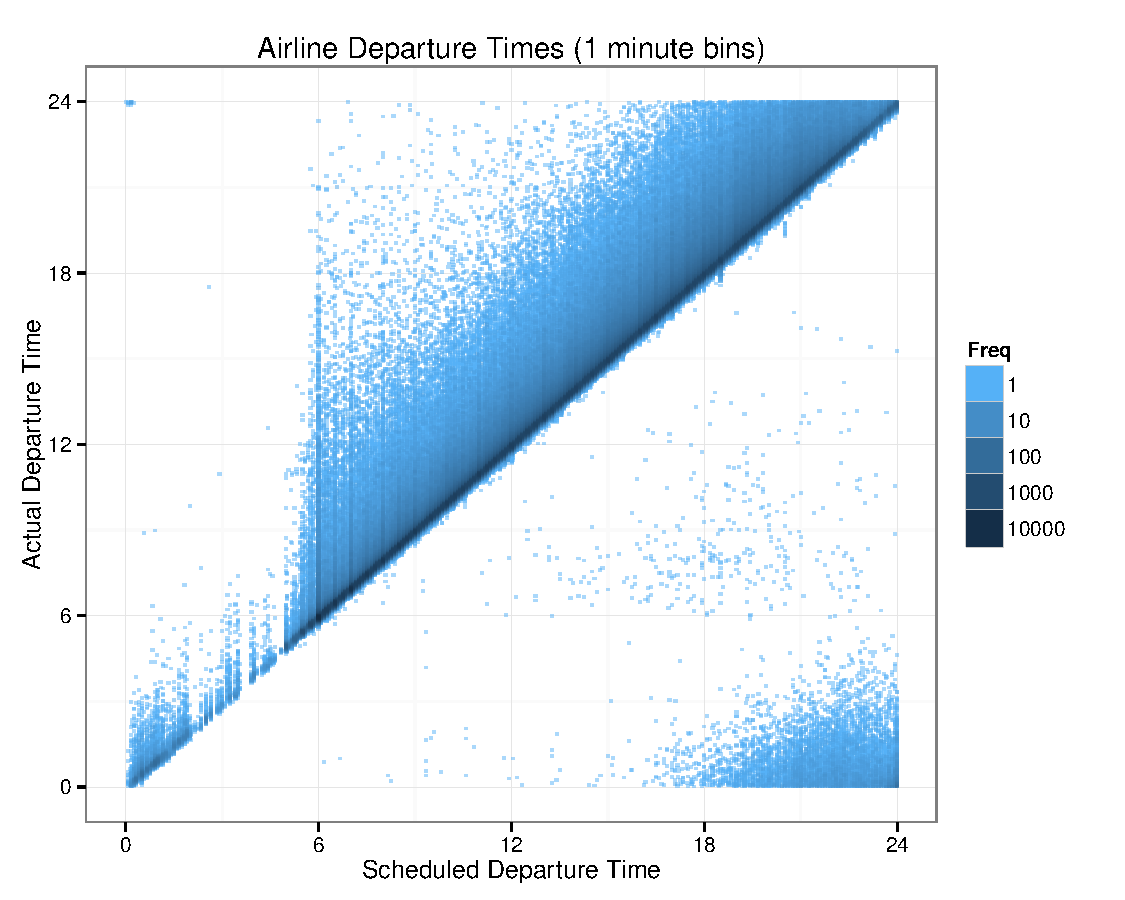
\includegraphics[width=.56\linewidth, keepaspectratio=TRUE]{BinnedScatter/AirlineStdBinning1min.pdf}}
\caption{\label{airline-scatter}Scheduled and actual departure times of  flights across the United States in 2011. The plot on the left is based on a sample of the data, the plot on the right shows all flights. The large scale distributional patterns are visible in both plots, but the plot on the left misses some of the finer level details in scheduling that is visible in the plot on the right.}
\end{figure}

Both plots show the same large scale distributional patterns: scheduled and actual arrival times are highly correlated, recognizable from the conglomeration of points along the identity line. Scheduled departure times past 6:00 am in the morning are much more common than earlier flights. It is much more likely for a  flight to be delayed than to leave early, leading to the wash-out effect above the line, that is getting thinner with increasing delays. The range of delays on usual days starts at about one hour at 6:00 am and increases during the day to about a two hour delay. The small number of flights before 6:00 am are also visible in both plots. The triangle of observations on the bottom right in both plots is nothing but an artifact of the data collection consisting of flights that are scheduled before midnight, but are delayed to departures past midnight. The cloud of outliers halfway between the two main structures is potentially interesting, since no immediate explanation comes to mind, and would be worthy of a follow-up investigation.

What is not apparent in the alpha-blended scatterplot, is some fine-level structure that the minimally binned scatterplot shows. Note that because we have bin widths equal to the resolution to which the data is recorded in each dimension, we know that the spatial binning algorithm will not cause any \textit{artificial} density stripes. A close inspection of the plot on the right hand side reveals darker colored vertical lines at 30 minute intervals. It is obvious that more flights are scheduled with departures on the hour and at 30 minutes past the hour. 

\begin{figure}[hbtp]\centering
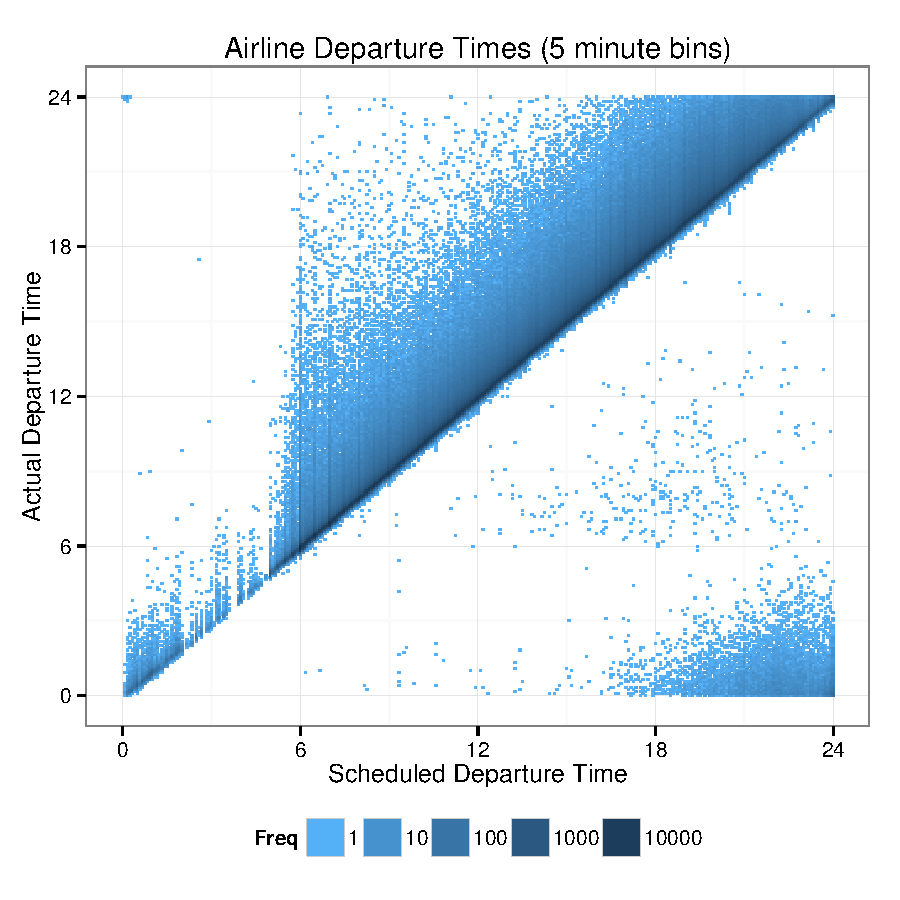
\includegraphics[width=.49\linewidth,keepaspectratio=true]{BinnedScatter/AirlineStdBinning5mins.pdf}
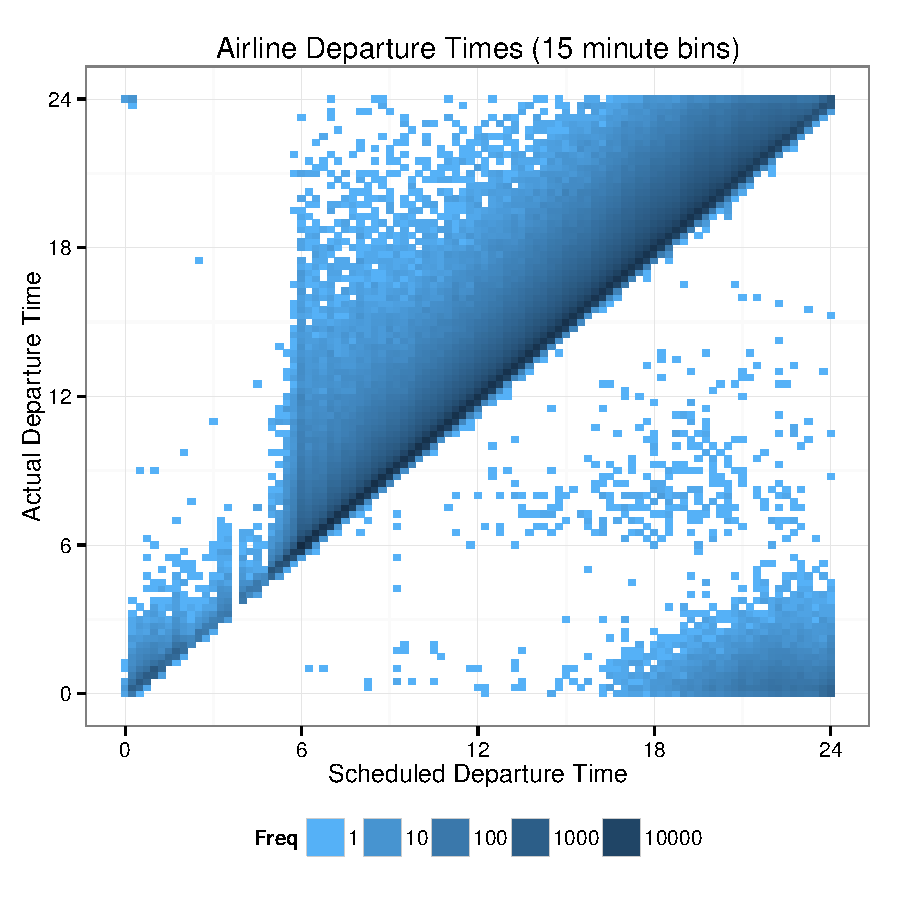
\includegraphics[width=.49\linewidth,keepaspectratio=true]{BinnedScatter/AirlineStdBinning15mins.pdf}
\caption{5-minute bins produce a higher-level summary of the data than shown in Figure~\ref{airline-scatter}b. 15-minute bins produce an even more coarse summary of the data.}\label{airline5mins-binning}
\end{figure}

Figure~\ref{airline5mins-binning} displays the binned scatterplots for the flight departure data with larger bins. Binning data by five-minute intervals produces a more high-level summary of the relationship between actual and scheduled departure time, though it necessarily obscures some of the finer details. In addition, binning data by five minute intervals reduces the size of the data set to a much more manageable 19,787 reduced binned data triples, which can be easily manipulated on probably any modern computer. Binning by 15-minute intervals reduces the data set to a nearly-trivial 3,575 reduced binned data triples, but the graphical summary becomes granular and less appealing at that resolution.



%--------------------------------------------------------------------------------------

\section{Conclusions and Future Work}

Large bivariate data sets are very difficult to visualize in raw form, due to over-plotting of points. Binning allows for the visualization and manipulation of large data sets, and easily translates into binned scatterplots which are more appropriate for the human visual system. Reducing the data for binned scatterplots has distinct computational and visual advantages, however the aggregation comes at the cost of losing precision in spatial and frequency information.

We have presented two algorithms for spatially binning data points; standard and random rectangular binning algorithms. The random binning algorithm displayed strong advantage of avoiding the problem of artificial stripes that occur when data recorded to a coarse resolution are binned using a bin width that was a non-integer multiple of the data resolution. However, the standard binning algorithm is superior due to lower spatial loss. For data with a coarse resolution ($\alpha_x$ units in the X dimension and $\alpha_y$ units in the Y dimension) artificial stripes in the standard binning process can be avoided, if  bin dimensions are chosen as integer multiples of $\alpha_x$ and $\alpha_y$.  We were also able to show through simulation that a reasonable default for the binning uses an origin offset of $(\alpha_x/2, \alpha_y/2)$ because it resulted in minimal or near minimal spatial loss for symmetric data and performed well even for spatially skewed data. 

Spatial binning with smaller bin dimensions will lead to lower spatial losses; however, finer binning requires more processing time and does not highlight large scale density structure. It is left to the plot designer to decide how much spatial information they are willing to sacrifice in order to simplify the display of density structure. %; we do however suggest to err on the side of smaller bins which allow for visualization of finer density structure with lower spatial loss.

If we elect to use frequency binning to shade tiles ordinally, it is recommended to use between four and seven distinct shades. This is done to minimize the frequency loss within the bounds of human perceptual ability to distinguish multiple shades simultaneously. Using quantile frequency binning or standard log frequency binning are shown to be reasonable methods -- with slight differences of interpretability -- for handling situations with heavily skewed bin counts.

Future implementations of software for constructing binned scatterplots would be well served to allow for choices in specification of binning algorithms. The findings of this research provide suggestions for reasonable default settings of binning parameters that maintain spatial and frequency information and lead to desirable visual properties in the binned scatterplot.

%----------------------------------------------------------------------------
% \newpage
% \begin{appendix}
% \section{Appendix}  
%   MOVED to Appendix1.Rnw file
% %----------------------------------------------------------------------------
% \subsection{Optimal Offset for Uniform Data Recorded to Resolution $\alpha$}
% \label{proof:offset}
% 
% The following is proof that when univariate data is uniformly distributed at resolution $\alpha$ and standard rectangular binning is used with binwidths that are a scalar multiple of the data resolution (i.e. $\omega = k\alpha$ for some $k \in \{1,2,\dots\})$, then spatial loss is minimized by setting the binning origin to $\alpha/2$ units below the minimum data value; set $\beta = x_{(1)} - \alpha/2$.
% 
% Let $x_1, x_2, \dots, x_k \in \mathbb{R}$ represent the values in a single bin such that $x_{i+1} = x_i + \alpha$ for some constant $\alpha \in \mathbb{R}$. Thus $x_j = x_1 + (j-1)\alpha$.
% 
% Suppose then that we bin the data using standard rectangular binning with origin, $\beta = x_1 - \theta$, and binwidth $\omega$; where $\theta$ is the \textit{origin offset} from the data. Thus $b(x_j) = \beta + \omega/2 = (x_1 - \theta) + (k\alpha/2)$
% 
% Spatial Loss, $L^S = \sum_{i=1}^{k} ||x_i-b_(x_i)|| $ is definitionally minimized when $b_(x_i)$ is the \textit{geometric median}. The geometric median for $x_1, \dots, x_k = Q_x(.5) = (x_{\lceil\frac{k+1}{2}\rceil}+x_{\lfloor \frac{k+1}{2}\rfloor})/2$ , where $Q_x(\cdot)$ is the empirical quantile function. 
% 
% Thus the optimal offset is the $\theta$ such that
% 
% $ b(x_i) = Q_x(.5) $ \\
% $ \Rightarrow (x_1 - \theta) + (k\alpha/2) = (x_{\lceil\frac{k+1}{2}\rceil}+x_{\lfloor \frac{k+1}{2}\rfloor})/2 $ \\
% $ \Rightarrow 2x_1 - 2\theta + k\alpha = (x_1 + (\lceil\frac{k+1}{2}\rceil - 1)\alpha ) + (x_1 + (\lfloor\frac{k+1}{2}\rfloor - 1)\alpha ) $ \\
% $ \Rightarrow -2\theta + k\alpha = (\lceil\frac{k+1}{2}\rceil - 1)\alpha  + (\lfloor\frac{k+1}{2}\rfloor - 1)\alpha  $ \\
% $ \Rightarrow -2\theta + k\alpha = ((k+1) - 2)\alpha  $ \\
% $ \Rightarrow -2\theta = -\alpha $ \\
% $ \Rightarrow \theta = \alpha/2 $ \\
% 
% Thus the optimal offset for reducing spatial loss in this scenario is $\theta = \alpha/2$.  This result holds for data that is symmetrically distributed within the bin since the median will not change.  It extends to multiple contiguous bins with resolution $\alpha$ data that has symmetrically distributed data withing each bin. 
% 
% If the same conditions are extended to the two dimensional case, then the origin for minimal spatial loss is at $(x_{(1)}-\alpha_x/2, y_{(1)}-\alpha_y/2)$ where $\alpha_x$ and $\alpha_y$  are the data resolution for each dimension, respectively. 
% 

\chaptocbreak

\chapter{CONCLUSIONS}
\label{ThesisEnd}

The goal at the onset of this dissertation was to overcome challenges and grasp opportunities associated with large data and emerging technology to advance the fields of statistics education and statistical graphics. The preceding chapters have demonstrated a successful pursuit of this goal through the review of existing literature to guide relevant research topics, the work to address difficult challenges in both fields, and the application of advanced statistical methods and analysis to draw actionable insights on each topic. To conclude, we review the primary results from each of the studies.

\km{The study on traditional and simulation-based statistical inference curricula took an ambitious and statistically rigorous approach to comparing learning outcomes through a designed experiment. The randomization of students to curricula helped to isolate the curricular effect by creating homogenous cohorts of students which received each curriculum. The student learning outcomes, measured using the ARTIST scaled questions sets for confidence intervals and hypothesis tests, were analyzed using a bivariate MANCOVA model which controls for pre-treatment factors, including scores from a midterm and lab. The model found no significant curriculum effect for learning outcomes related to hypothesis tests; despite the added complexity in the simulation-based curriculum. The model also indicates a statistically significant 7\% improvement on the ARTIST scale for the simulation-based curriculum over the traditional curriculum for learning outcomes related to confidence intervals, while accounting for pre-treatment covariates. However, the validity of these results is highly questionable because the model assumption of independence between students is likely untrue. The simulation study demonstrated that the Type I error rates in tests for curricular effects inflate dramatically under minor violations that have lecture or lab section based variance structure. Therefore, caution must be taken in interpreting the results of this study which are suggestive, but not conclusive, of a simulation-based curriculum benefit.}

The Shiny Database Sampler stands as a successful proof of concept that big data sources can be incorporated into an introductory statistics curriculum. The web-based interface is designed to allow students to easily obtain samples from large databases, using random sampling methodology to infuse the software with pedagogical value. Course activities for an introductory statistics course were also developed to incorporate and leverage the Shiny Databases Sampler for learning about sampling concepts. The software was assessed through a student user survey designed to measure the ease of use, connection to sampling concepts and the engagement with the data. The survey indicates that students find the Shiny Database Sampler easy to use, notice the connection to sampling concepts and are moderately engaged with the data context.

The research on loss related to the construction of binned scatterplots yielded interesting exploration of loss properties and several recommendations for binning specification. Traditional scatterplots are fundamentally unable to scale for large data due to over-plotting which obscures frequency information. Binned scatterplots trade individual points for shaded tiles, sacrificing exact data locations to allow frequency information to be displayed. The spatial loss is measured as the sum of Euclidean distances from points to the bin centers. Bin frequency information can be rendered precisely through continuous shading, however the perceptual ability to extract that information is imperfect. We propose the use of frequency binning to make this imprecision explicit, thus allowing the measurement of frequency loss. The exploration of loss properties provides a few main recommendations for binning specifications: bin dimensions should be integer multiples of the data resolution, it is often beneficial to offset the binning origin by half the data resolution in each dimension, quantile and standard log frequency binning are two viable strategies for dealing with heavily skewed bin frequencies, and four to seven frequency groups should be used when frequency binning is employed.

This research contributes to methodology in statistics education and statistical graphics. While the research goal of this dissertation was successfully pursued, there remain many challenges and opportunities within these fields that provide abundant avenues for future work. 
\chaptocbreak

\appendixtitle
\begin{appendices}
\appendix

% Appendix1 file from standard thesis template
\chapter{ }



%-------------------------------------------------------

\section{Appendix: Final Exam Used in Curricula Study}
\label{appendA}

The following appendix contains the questions and point rubrics for the ARTIST scaled questions and the applied theory-based inference problems as they appeared on the final exam.

\subsection{ARTIST Scaled Multiple Choice Question Set for Confidence Intervals}
\label{appendA1}

1. Answer the following general multiple choice questions regarding confidence intervals.  There is only one correct answer for each (circle the best option).

i. Two different samples will be taken from the same population of test scores where the population mean and standard deviation are unknown. The first sample will have 25 data values, and the second sample will have 64 data values. A 95\% confidence interval will be constructed for each sample to estimate the population mean. Which confidence interval would you expect to have greater precision (a smaller width) for estimating the population mean?

a. I expect the confidence interval based on the sample of 64 data values to be more precise.\\
b. I expect both confidence intervals to have the same precision.\\
c. I expect the confidence interval based on the sample of 25 data values to be more precise.\\

ii. A 95\% confidence interval is computed to estimate the mean household income for a city. Which of the following values will definitely be within the limits of this confidence interval?

a. The population mean\\
b. The sample mean\\
c. The standard deviation of the sample mean\\
d. None of the above\\

iii. Each of the 110 students in a statistics class selects a different random sample of 35 Quiz scores from a population of 5000 scores they are given. Using their data, each student constructs a 90\% confidence interval for $\mu$ the average Quiz score of the
5000 students. Which of the following conclusions is correct?

a. About 10\% of the sample means will not be included in the confidence intervals.\\
b. About 90\% of the confidence intervals will contain $\mu$.\\
c. It is probable that 90\% of the confidence intervals will be identical.\\
d. About 10\% of the raw scores in the samples will not be found in these confidence intervals\\

iv. A 95\% confidence interval for the mean reading achievement score for a population of third grade students is (43, 49). The margin of error of this interval is:

a. 5\\
b. 3\\
c. 6\\

v. Justin and Hayley conducted a mission to a new planet, Planet X, to study arm length. They took a random sample of 100 Planet X residents and calculated a 95\% confidence interval for the mean arm length. What does a 95\% confidence interval for arm length tell us in this case? Select the best answer:

a. I am 95\% confident that this interval includes the sample mean (x) arm length.\\
b. I am confident that most (95\%) of all Planet X residents will have an arm length within this interval.\\
c. I am 95\% confident that most Planet X residents will have arm lengths within this interval.\\
d. I am 95\% confident that this interval includes the population mean arm length.\\


vi. Suppose that a random sample of 41 state college students is asked to measure the length of their right foot in centimeters. A 95\% confidence interval for the mean foot length for students at this university turns out to be (21.709, 25.091). If instead a 90\% confidence interval was calculated, how would it differ from the 95\% confidence interval?

a. The 90\% confidence interval would be narrower.\\
b. The 90\% confidence interval would be wider.\\
c. The 90\% confidence interval would be the same as the 95\% confidence interval.\\


vii. A pollster took a random sample of 100 students from a large university and computed a confidence interval to estimate the percentage of students who were planning to vote in the upcoming election. The pollster felt that the confidence interval was too wide to provide a precise estimate of the population parameter. What could the pollster have done to produce a narrower confidence interval that would produce a more precise estimate of the percentage of all university students who plan to vote in the upcoming election?

a. Increase the sample size to 150.\\
b. Increase the confidence level to 99\%.\\
c. Both a and b\\
d. None of the above\\


viii. A newspaper article states with 95\% confidence that 55\% to 65\% of all high school students in the United States claim that they could get a hand gun if they wanted one. This confidence interval is based on a poll of 2000 high school students in Detroit. How would you interpret the confidence interval from this newspaper article?

a. 95\% of large urban cities in the United States have 55\% to 65\% high school students who could get a hand gun.\\
b. If we took many samples of high school students from different urban cities, 95\% of the samples would have between 55\% and 65\% high school students who could get hand guns.\\
c. You cannot use this confidence interval to generalize to all teenagers in the United States because of the way the sample was taken.\\
d. We can be 95\% confident that between 55\% and 65\% of all United States high school students could get a hand gun.\\

ix. The Gallup poll (August 23, 2002) reported that 53\% of Americans said they would favor sending American ground troops to the Persian Gulf area in an attempt to remove Hussein from power. The poll also reported that the margin of error for this poll was 4\%. What does the margin of error of 4\% indicate?

a. There is a 4\% chance that the estimate of 53\% is wrong.\\
b. The percent of Americans who are in favor is probably higher than 53\% and closer to 57\%.\\
c. The percent of Americans who are in favor is estimated to be between 49\% and 57\%.\\

x. Suppose two researchers want to estimate the proportion of American college students who favor abolishing the penny. They both want to have about the same margin of error to estimate this proportion. However, Researcher 1 wants to estimate with 99\% confidence and Researcher 2 wants to estimate with 95\% confidence. Which researcher would need more students for her study in order to obtain the desired margin of error?

a. Researcher 1.\\
b. Researcher 2.\\
c. Both researchers would need the same number of subjects.\\
d. It is impossible to obtain the same margin of error with the two different confidence levels.\\

\subsection{ARTIST Scaled Multiple Choice Question Set for Hypothesis Testing}

2.   Answer the following general multiple choice questions regarding hypothesis testing.  There is only one correct answer for each (circle the best option).  As a helpful note the term ``statistically significant'' means that you reject the null hypothesis.

i. The makers of Mini-Oats cereal have an automated packaging machine that is set to fill boxes with 24 ounces of cereal. At various times in the packaging process, a random sample of 100 boxes is taken to see if the machine is filling the boxes with an average of 24 ounces of cereal. Which of the following is a statement of the null hypothesis being tested?

a. The machine is filling the boxes with the proper amount of cereal.\\
b. The machine is not filling the boxes with the proper amount of cereal.\\
c. The machine is not putting enough cereal in the boxes.\\

ii. A research article gives a p-value of .001 in the analysis section. Which definition of a p-value is the most accurate?

a. the probability that the observed outcome will occur again.\\
b. the probability of observing an outcome as extreme or more extreme than the one observed if the null hypothesis is true.\\
c. the value that an observed outcome must reach in order to be considered significant under the null hypothesis.\\
d. the probability that the null hypothesis is true.\\

iii. If a researcher was hoping to show that the results of an experiment were statistically significant they would prefer:

a. a large p-value\\
b. a small p-value\\
c. p-values are not related to statistical significance\\


iv. A researcher compares men and women on 100 different variables using a difference in means t-test.  He sets the level of significance at 0.05 and then carries out 100 independent t-tests (one for each variable) on these data.  If, for each test, the null hypothesis is actually true, about how many ``statistically significant'' results will be produced?

a. 0\\
b. 5\\
c. 10\\
d. none of the above\\

Problems (v) and (vi) refer to the following situation: Food inspectors inspect samples of food products to see if they are safe. This can be thought of as a hypothesis test where Null: the food is safe, and Alternative: the food is not safe. Identify each of the following statements as a Type I or a Type II error.

v. The inspector says the food is safe but it actually is not safe.

a. Type I\\
b. Type II\\

vi. The inspector says the food is not safe but is actually safe.

a. Type I\\
b. Type II\\

vii. A newspaper article claims that the average age for people who receive food stamps is 40 years. You believe that the average age is less than that. You take a random sample of 100 people who receive food stamps, and find their average age to be 39.2 years. You find that this is significantly lower than the age of 40 stated in the article (p-value < .05). What would be an appropriate interpretation of this result?

a. The statistically significant result indicates that the majority of people who receive food stamps is younger than 40.\\
b. Although the result is statistically significant, the difference in age is not of practical importance.\\
c. An error must have been made. This difference is too small to be statistically significant.\\

viii. A newspaper article stated that the US Supreme Court received 812 letters from around the country on the subject of whether to ban cameras from the courtroom. Of these 812 letters, 800 expressed the opinion that cameras should be banned. A statistics student was going to use this sample information to conduct a test of significance of whether more than 95\% of all American adults feel that cameras should be banned from the courtroom. What would you tell this student?

a. This is a large enough sample to provide an accurate estimate of the American public's opinion on the issue.\\
b. The necessary conditions for a test of significance are not satisfied, so no statistical test should be performed.\\
c. With such a large number of people favoring the notion that cameras be banned, there is no need for a statistical test.\\

ix. A researcher conducts an experiment on human memory and recruits 15 people to participate in her study. She performs the experiment and analyzes the results. She obtains a p-value of .17. Which of the following is a reasonable interpretation of her results?

a. This proves that her experimental treatment has no effect on memory.\\
b. There could be a treatment effect, but the sample size was too small to detect it.\\
c. She should reject the null hypothesis.\\
d. There is evidence of a small effect on memory by her experimental treatment.\\

x. It is reported that scores on a particular test of historical trivia given to high school students are approximately normally distributed with a mean of 85. Mrs. Rose believes that her 5 classes of high school seniors will score significantly better than the national average on this test. At the end of the semester, Mrs. Rose administers the historical trivia test to her students. The students score an average of 89 on this test. After conducting the appropriate statistical test, Mrs. Rose finds that the p-value is .0025. Which of the following is the best interpretation of the p-value?

a. A p-value of .0025 provides strong evidence that Mrs. Rose's class outperformed high school students across the nation.\\
b. A p-value of .0025 indicates that there is a very small chance that Mrs. Rose's class outperformed high school students across the nation.\\
c. A p-value of .0025 provides evidence that Mrs. Rose is an exceptional teacher who was able to prepare her students well for this national test.\\
d. None of the above.\\


\subsection{Applied Theory-Based Confidence Interval Question}

3. Farmer Cindy is in charge of the chickens on her family's farm, and is curious about the average number of eggs the entire flock produces in a month.  Observing the entire flock would be time consuming, so she approaches you asking what her options are. You inform her that 30 chickens should be selected at random to be observed for a month. After the month she observes the average number of eggs her sample of 30 chickens produced is 25 eggs with a standard deviation of 6 eggs.  
\begin{enumerate} 
\item (5 pts) Construct a 95\% confidence interval for the average number of eggs chickens from her entire population produce in a month.  (You don't need to check any conditions here)  
\item (3 pts) Interpret the 95\% confidence interval constructed in the previous part:
\item (2 pts) Cindy is disappointed with the width of the interval you provide for her, suggest to her two ways she could obtain a narrower confidence interval.
\end{enumerate}

\subsection{Applied Theory-Based Hypothesis Testing Question}

4. Cindy becomes concerned about a disease some of her chickens are catching that causes a decrease in the chicken's egg production.  She is interested in the proportion of her entire flock that has the disease, but detecting the disease requires taking blood from the chicken which is expensive and time consuming.  After working with you in the past, she understands that she can estimate this proportion by taking just a sample of her chickens! Assume she selects a sample of 100 chickens in the best possible way and observed that 15 of the chickens had the disease.

Cindy's pessimistic guess is that 25\% of the flock has the disease.  Complete the following steps to test if the proportion of her entire population diseased is less than 0.25.  
\begin{enumerate} 
\item (2 pts) State the Null and Alternative hypothesis:
\item (2 pts) Check the conditions for a hypothesis test:
\item (2 pts) Calculate the test statistic:
\item (2 pts) Find the p-value:
\item (3 pts) Make a decision about your hypothesis and state your conclusion in context of the problem. 
\end{enumerate}

%-------------------------------------------------------

\section{Appendix: Midterm Exam Used in Curricula Study}
\label{appMidtermExamQuestions}

The following appendix is the midterm exam in its entirety, along with point designations for each question.  Note that Problem 6 for the midterm is the ARTIST scaled question set for assessing topics related to "data collection". This ARTIST set was included with the goal to strengthen the midterm as a effective covariate for controlling for pre-treatment differences in the curricula groups in the model comparing learning outcomes using the ARTIST scores. 

%load packages that will be invisible on slides


%---------------------------------------------------------------------

\textbf{1. [28 points] Linear Regression:} A study was conducted in England in 1989 investigating the relationship between smoking and lung cancer mortality within different occupational groups of males. The data include a smoking index and a lung cancer mortality index for men in 25 occupational groups in England. \\
\indent The smoking index measures the percentage of the number of cigarettes smoked per day by men in the particular occupational group compared to the average number of cigarettes smoked per day by all men. The units associated with the smoking index are percent of average cigarettes smoked (\% avg CS).  The mortality index measures the percentage of the rate of deaths from lung cancer among men in the particular occupational group compared to the rate of deaths from lung cancer among all men. The units associated with the mortality index are percent of average lung cancer deaths (\% avg LCD).  \\
\indent The data for the 25 occupations are displayed in the scatterplot below. Use the information from the scatterplot, the sample statistics and linear regression equation listed below to answer all parts of this problem. \\
\begin{knitrout}
\definecolor{shadecolor}{rgb}{0.969, 0.969, 0.969}\color{fgcolor}

{\centering \includegraphics[width=.5\linewidth]{Figureregprobplot-1} 

}



\end{knitrout}
\begin{table}[hbtp]\centering 
\begin{tabular}{ |c|c|c|}
  \hline                        
 $\bar{x}$ = 102.88\% avg CS & $\bar{y}$ = 109\% avg LCD & r=0.7162\\
 $S_x$ = 17.1982 \% avg CS & $S_y$ = 26.1135\% avg LCD & $R^2$ = 0.5129\\
  \hline  
\end{tabular}
\end{table}

\begin{center}
\textbf{Prediction Equation:} \hspace{.2in}  $\hat{y} = \ensuremath{-2.8853189} + x(1.0875323)$
\end{center}
\noindent\textbf{(a)} [2 points] What is the response variable?\\
\noindent\textbf{(b)} [2 points] What is the explanatory variable?\\
\noindent\textbf{(c)} [4 points] The correlation coefficient, r=0.7162.  Using this value, what can be said about the relationship between the smoking index and the lung cancer mortality index?\\
\noindent\textbf{(d)} [4 points] The slope of the linear regression model is 1.0875323. Show the calculations to prove that this is the value for the slope. Then, interpret this value in the context of the problem.\\
\noindent\textbf{(e)} [4 points] The intercept of the linear regression model is \ensuremath{-2.8853189}. First, show the calculations to prove that this is the value for the intercept. If it is appropriate to interpret this value in the context of the problem, then do so. Otherwise, specify why it is inappropriate to interpret this value.\\
\noindent\textbf{(f)} [3 points] In the prediction equation for the regression line explain that the symbols $\hat{y}$ and x represent.\\
\noindent\textbf{(g)} [3 points] Using the prediction line given above, predict the morality index (in \% avg LCD) for an occupational group that has a smoking index of 110\% avg CS (round your answer to 2 decimal places).\\
\noindent\textbf{(h)} [3 points] Suppose that there was an occupational group in our data set with a smoking index of 110\% avg CS and a mortality index of 140\% avg LCD.  Calculate the residual for this occupational group (round your answer to 2 decimal places).\\
\noindent\textbf{(i)} [3 points] Interpret the $R^2$ value in terms of the context of the problem.\\
%--------------------------------------------------------------------------

\textbf{2. [10 points]} A Gallup poll conducted on February 26, 2014 investigated the wellbeing of American adults. The survey used the Gallup-Healthways Well-Being Index to classify the person's wellbeing as "thriving", "struggling" or "suffering". The telephone survey found that 55\% of 1500 randomly selected American adults were classified as thriving.  \\
For this study, identify the following:\\
\noindent\textbf{(a)} [2 points] Identify the population of interest.\\
\noindent\textbf{(b)} [2 points] Identify the sample.\\
\noindent\textbf{(c)} [2 points] Identify the population parameter.\\
\noindent\textbf{(d)} [2 points] Identify the sample statistic.\\
\noindent\textbf{(e)} [2 points] Identify the variable.\\

%--------------------------------------------------------------------------

\textbf{3. [10  points]} A study investigated the relationship between heights of husbands and wives. Heights were recorded as groupings of "Tall", "Medium" and "Short". The researcher recorded height pairings for 205 married couples and wants to know how the height of the husband associated the height of the wife. Use the information found in the contingency table below to answer the questions that follow.
\begin{table}[hbtp]\centering 
\begin{tabular}{ |cc|ccc|c|}
  \hline                        
  & & & Wife & & \\
  & & Tall & Medium & Short & Total \\
 \hline
          & Tall    & 18 & 28  & 14  & 60  \\
Husband   & Medium  & 20 & 51  & 28  & 99  \\
          & Short   & 12 & 25  & 9   &  46 \\
  \hline  
  & Total & 50 & 104 & 51 & 205 \\
  \hline
\end{tabular}
\end{table}
\noindent\textbf{(a)} [2  points] What is the probability that a randomly selected married couple will have a short husband?\\
\noindent\textbf{(b)} [2  points] What is the probability that a randomly selected married couple will have a tall wife \textit{and} a short husband?\\
\noindent\textbf{(c)} [2  points] What is the probability that a randomly selected married couple will have a tall wife \textit{or} a short husband?\\
\noindent\textbf{(d)} [2  points] What is the probability that a randomly selected married couple will have a short husband \textit{given} that we know the wife is tall?\\
\noindent\textbf{(e)} [2  points] Are the events of short husband and tall wife \textit{independent}? Justify your answer mathematically.\\

%--------------------------------------------------------------------------

\textbf{4. [8 points]} Suppose that we have a box containing 23 marbles of equal size and shape so that each marble is equally likely to be selected from the box.  There are 10 red, 8 green, 3 yellow marbles and  2 black marbles.  Suppose we assign points to each color marble: 2 points for a red, 5 point for a green, 10 points for a yellow and 15 points for a black. Let X be the discrete random variable that counts the number of points that a randomly selected marble is worth.\\
\noindent\textbf{(a)} [2 points] Find the probability distribution of X? (fill out table and round all values to 2 decimal places)
\begin{table}[hbtp]\centering 
\begin{tabular}{ c|c }
x & P(x) \\
  \hline  
   &  \\
   &  \\
   &  \\  
\end{tabular}
\end{table}
\noindent\textbf{(b)} [4 points] What 2 properties must be true for the values in the P(x) column of the probability distribution in part 4(a)? Note that X is a discrete random variable.\\
\noindent\textbf{(c)} [2 points] What is the mean of X? (If you were unable to complete part 4(a), describe how you would find the mean) \\

%---------------------------------------------------------------------

\textbf{5. [10 points]} A survey on gender and income was conducted and a random sample of 3700 Adult U.S. residents was gathered. In the figure below are side-by-side boxplots of the income (in thousands of dollars) for male and female U.S. residents. Use this graphical display to answer the following questions.
\begin{knitrout}
\definecolor{shadecolor}{rgb}{0.969, 0.969, 0.969}\color{fgcolor}

{\centering \includegraphics[width=.8\linewidth]{Figuresidebysidebox-1} 

}



\end{knitrout}
\begin{table}[H]\centering 
\begin{tabular}{ |c||c|c||c|c|c|c|c|}
  \hline                        
Gender  & mean & sd & min & Q1 & median & Q3 & max \\
 \hline
 Male & 39319 & 54242 & -10000 & 12000 & 25600 & 46700 & 685000 \\
 Female & 18786 & 21570 & -10000 & 4880 & 13500 & 25800 & 239000 \\
  \hline
\end{tabular}
\end{table}
\noindent\textbf{(a)} [5 points] Using full sentences, describe the distribution of income for \textit{only} the male residents of the U.S.  \\
\noindent\textbf{(b)} [5 points] Using full sentences, compare the distribution of male and female distributions of income. A complete answer will compare shapes, centers and spreads. Be specific about which measures of center and spread are being used to make these comparisons. (ie writing "the spread is bigger" will not earn full credit)  \\

%--------------------------------------------------------------------------

\underline{\textbf{6. [18 points]} Multiple Choice: \textit{Clearly} circle the selected answer.}\\
\noindent\textbf{(i)} [2 points] In a survey people are asked 'Which brand of toothpaste do you prefer?' The data gathered from this question would be what type of data? \\
\indent a. continuous \\
\indent b. categorical \\
\indent c. quantitative 

\textbf{Items ii and iii refer to the following situation:}
A student is gathering data on the driving experiences of other college students. One of the variables measured is the type of car the student drives. These data are coded using the following method: 1 = subcompact, 2 = compact, 3 = standard size, 4 = full size, 5 = premium, 6 = mini van, 7 = SUV, and 8 = truck.

\noindent\textbf{(ii)} [2 points] What type of variable is this? \\
\indent a. categorical \\
\indent b. quantitative \\
\indent c. continuous 

\noindent\textbf{(iii)} [2 points] The student plans to see if there is a relationship between the number of speeding tickets a student gets in a year and the type of vehicle he or she drives. Identify the response variable in this study. \\
\indent a. college students \\
\indent b. type of car \\
\indent c. number of speeding tickets \\
\indent d. average number of speeding tickets last year 

\noindent\textbf{(iv)} [2 points] A researcher is studying the relationship between a vitamin supplement and cholesterol level. What type of study needs to be done in order to establish that the amount of vitamin supplement causes a change in cholesterol level? \\
\indent a. Survey \\
\indent b. Randomized experiment \\
\indent c. Time Series Study \\
\indent d. Survey 

\noindent\textbf{(v)} [2 points] An instructor is going to model an experiment in his statistics class by comparing the effect of 4 different treatments on student responses. There are 40 students in the class. Which is the best way for the instructor to distribute the students to the 4 treatments for this experiment? \\ 
\indent a. Assign the first treatment to the first 10 students on the class list, the second treatment to the next 10 students, and so on. \\
\indent b. Assign a unique number to each student, then use random numbers to assign 10 students to the first treatment, 10 students to the second treatment, and so on. \\
\indent c. Assign the treatment as students walk into class, giving the first treatment to the first 10 students and the second treatment to the next 10 student, and so on. \\
\indent d. All of these are equally appropriate methods. \\
\indent e. None of these is an appropriate method.

\textbf{Items vi and vii refer to the following situation:}\\
Suppose two researchers wanted to determine if aspirin reduces the chance of a heart attack.

\noindent\textbf{(vi)} [2 points] Researcher 1 studied the medical records of 500 randomly selected patients. For each patient, he recorded whether the person took aspirin every day and if the person had ever had a heart attack. Then he reported the percentage of heart attacks for the patients who took aspirin every day and for those who did not take aspirin every day. What type of study did Researcher 1 conduct? \\ 
\indent a. Observational \\
\indent b. Experimental \\
\indent c. Survey \\
\indent d. None of the above

\noindent\textbf{(vii)} [2 points] Researcher 2 also studied 500 patients that visited a regional hospital in the last year. He randomly assigned half (250) of the patients to take aspirin every day and the other half to take a placebo everyday. Then after a certain length of time he reported the percentage of heart attacks for the patients who took aspirin every day and for those who did not take aspirin every day. What type of study did Researcher 2 conduct? \\ 
\indent a. Observational \\
\indent b. Experimental \\
\indent c. Survey \\
\indent d. None of the above 

\noindent\textbf{(vii)} [2 points] The dean of a college would like to determine the feelings of students concerning a new registration fee that would be used to upgrade the recreational facilities on campus. All registered students would pay the fee each term. Which of the following data collection plans would provide the best representation of students' opinions at the school? \\
\indent a. Survey every 10th student who enters the current recreational facilities between the hours of 1:00 and 5:00 pm until 100 students have been asked. \\
\indent b. Randomly sample fifty student ID numbers and send a survey to all students in the sample. \\
\indent c. Place an ad in the campus newspaper inviting students to complete an online survey. Collect the responses of the first 200 students who respond. \\
\indent d. All of the above would be equally effective. 

\noindent\textbf{(ix)} [2 points] A team in the Department of Institutional Review at a large university wanted to study the relationship between completing an internship during college and students' future earning potential. From the same graduating class, they selected a random sample of 80 students who completed an internship and 100 students who did not complete an internship and examined their salaries 5 years past graduation. They found that there was a statistically higher mean salary for the internship group than for the non-internship group. Which of the following interpretations do you think is the most appropriate?\\
\indent a. More students should take internships because having an internship produces a higher salary.\\
\indent b. There could be a confounding variable, such as student major, that explains the difference in mean salary between the internship and no internship groups. \\
\indent c. You cannot draw any valid conclusions because the samples are not the same size.\\

%--------------------------------------------------------------------------

\textbf{7. [8 points]} When playing the game Settlers of Catan\textbf{TM} there is a game piece known as the robber that blocks resources from being obtained.  On each player's turn, that player rolls a pair of 6 sided dice.  If the sum of the dice roll equals 7 then that player may move the robber. This means that there is a 6/36 chance of moving the robber with every roll of the dice, because there are 6 of the 36 possible combinations that sum to 7. Let X count the number of times that one player moves the robber in 12 turns.\\
\noindent\textbf{(a)} [4 points]  Check the 4 conditions to argue that X is a Binomial Random Variable  \\
\noindent\textbf{(b)} [2 points]  What is the probability that a player gets to move the robber 2 times during the 12 turns?  \\
\noindent\textbf{(c)} [2 points]  What is the mean number of times during 12 turns that a player will be able to move the robber?\\

%-----------------------------------------------------------------------

\textbf{8. [4 points]} A waiter from a restaurant keeps track of the information about tips he receives from dinning parties. Part of this data includes the tipping rate, as a proportion of the total bill, that was tipped. Below is a histogram of tipping rates from the 244 dinning parties served by the waiter. Use this histogram to answer the following question.
\begin{knitrout}
\definecolor{shadecolor}{rgb}{0.969, 0.969, 0.969}\color{fgcolor}

{\centering \includegraphics[width=.7\linewidth]{Figuretipratehisto-1} 

}



\end{knitrout}
\noindent\textbf{(a)} [2 points]  What is the best measure of center to describe the distribution of tipping rates? Explain your answer. (Note: no calculations or estimated values are needed to answer this problem)  \\
\noindent\textbf{(b)} [2 points]  What is the best measure of spread to describe the distribution of tipping rates? Explain your answer. (Note: no calculations or estimated values are needed to answer this problem) \\

%-----------------------------------------------------------------------

\textbf{9. [4 points]} Below are histograms for two separate random samples of 30 quiz scores.  Which quiz will have the larger sample standard deviation for quiz scores? \textbf{Explain your choice briefly}. (Note: You do not, and should not, do any calculations to answer this question)
\begin{figure}[H]
\begin{center}
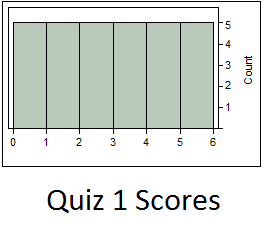
\includegraphics[keepaspectratio=TRUE,width=.2\textwidth]{CurriculumStudy/QuizScores1Version1.png}
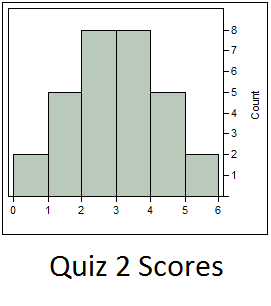
\includegraphics[keepaspectratio=TRUE,width=.2\textwidth]{CurriculumStudy/QuizScores2Version1.png}
\end{center}
\end{figure}

%-------------------------------------------------------
\section{Appendix: MANCOVA Model Diagnostics}
\label{appModDiag}

For the ARTIST Model described in Subsection~\ref{ArtistModel} and the Applied Model described in Subsection~\ref{AppliedModel} a set of model diagnostics were conducted. Each of these MANCOVA models are parameterized as specified in Section~\ref{analysis}; as such the assessment of model assumptions will be very similar for each model.   Residual plots will be used to assess the assumptions of linearity and constant variance.  The univariate and bivariate normality of the error terms will be assessed visually using normal quantile plots and a scatterplot of the paired residuals from the model. Additionally, although it is not a modeling assumption, MANCOVA models are best behaved with low to moderate correlation between the response variables, because then then model is able to capture variance unique to each response. 

% \subsection{Simulation Study for Violations of Independence}
% \label{simappend}
% 
% \km{To be removed after new simulation section added to main body.}\\
% 
% The ARTIST Model of the form (\ref{eq:mancova}) assumes  that errors from different students are independent, i.e.~$\Cov[\epsilon_{ik}, \epsilon_{jl}] = 0$, for all $i \neq j$ with $ 1 \le i,j \le n$. In our simulation setting, we simulate data from a model adapted from the model~(\ref{eq:mancova}), where there is no curriculum effect, i.e.~$\tau_{1} =  \tau_{2} = 0$ and where additionally the assumption of independent errors is violated by assuming a between student covariance of 
% \[
% \Cov[\epsilon_{ik}, \epsilon_{jl}] = \eta \sigma_{kl}^2, \ \ \ \text{ where } \eta \in [0,1]  \text{ for all } i \ne j. 
% \]
% $\eta$ scales the covariance between all students uniformly and can be adjusted to increase the violation of independence. Note that when $\eta = 0$ we have no violation of independence. Thus our generative model for the ARTIST responses are linear combinations of the midterm and lab~5 scores with correlated errors. This generative model for simulation can be organized using vector notation as follows:
% %
% \begin{eqnarray}\label{eq:linear}
% \begin{bmatrix}
%   \vec{y}_1 \\ \vec{y}_2
%   \end{bmatrix}  = 
% % %---- 
% \begin{bmatrix}
%  y_{11} \\ \vdots \\ y_{n1} \\ y_{12} \\ \vdots \\ y_{n2} 
% \end{bmatrix}  =
% % %----  
%  \begin{bmatrix}
%   \beta_{01} + x_{11}\beta_{11} + x_{12}\beta_{21}  \\
%   \vdots  \\ 
%   \beta_{01} + x_{n1}\beta_{11} + x_{n2}\beta_{21}  \\
%   \beta_{02} + x_{11}\beta_{12} + x_{12}\beta_{22}  \\
%   \vdots  \\ 
%   \beta_{02} + x_{n1}\beta_{12} + x_{n2}\beta_{22}  \\
%  \end{bmatrix} +
%  \begin{bmatrix}
%  \epsilon_{11} \\ \vdots \\ \epsilon_{n1} \\ \epsilon_{12} \\ \vdots \\ \epsilon_{n2} 
%  \end{bmatrix} = 
%  % %----
%  \begin{bmatrix}
%   X\vec{\beta}_1 \\ X\vec{\beta}_2
%   \end{bmatrix} + 
%   \vec{\epsilon},
% \end{eqnarray} 
% %
% \begin{eqnarray}\label{eq:error}
% \vec{\epsilon} \sim
% % %----  
%  \text{MVN}\left(
% \vec{0} \hspace{.1cm}
%   , 
%   \begin{bmatrix}
%    \sigma_{11}^2 & \sigma_{12}^2 \\ 
%    \sigma_{21}^2 & \sigma_{22}^2
%   \end{bmatrix}
% \otimes
%  \left( \eta 1_{n \times n} + (1- \eta) I_{n \times n}\right)
% %  \left[\begin{array}{ccccc|ccccc}
% %   \sigma_{11}^2 & \eta \sigma_{11}^2 & \cdots & \eta \sigma_{11}^2 & \eta \sigma_{11}^2 & \sigma_{12}^2 & \eta \sigma_{12}^2 & \cdots & \eta \sigma_{12}^2 & \eta \sigma_{12}^2\\
% %   \eta \sigma_{11}^2 & \sigma_{11}^2 & \ddots & \eta \sigma_{11}^2 & \eta \sigma_{11}^2 & \eta \sigma_{12}^2 & \sigma_{12}^2 & \ddots & \eta \sigma_{12}^2 & \eta \sigma_{12}^2\\
% % \vdots & \ddots & \ddots &\ddots &\vdots & \vdots & \ddots & \ddots &\ddots &\vdots \\
% % \eta \sigma_{11}^2 & \eta \sigma_{11}^2 & \ddots & \sigma_{11}^2 & \eta \sigma_{11}^2 & \eta \sigma_{12}^2 & \eta \sigma_{12}^2 & \ddots & \sigma_{12}^2 & \eta \sigma_{12}^2\\
% % \eta \sigma_{11}^2 & \eta \sigma_{11}^2 & \cdots & \eta \sigma_{11}^2 & \sigma_{11}^2 & \eta \sigma_{12}^2 & \eta \sigma_{12}^2 & \cdots & \eta \sigma_{12}^2 & \sigma_{12}^2\\
% % \hline
% % \sigma_{12}^2 & \eta \sigma_{12}^2 & \cdots & \eta \sigma_{12}^2 & \eta \sigma_{12}^2 & \sigma_{22}^2 & \eta \sigma_{22}^2 & \cdots & \eta \sigma_{22}^2 & \eta \sigma_{22}^2\\
% %   \eta \sigma_{12}^2 & \sigma_{12}^2 & \ddots & \eta \sigma_{12}^2 & \eta \sigma_{12}^2 & \eta \sigma_{22}^2 & \sigma_{22}^2 & \ddots & \eta \sigma_{22}^2 & \eta \sigma_{22}^2\\
% % \vdots & \ddots & \ddots &\ddots &\vdots & \vdots & \ddots & \ddots &\ddots &\vdots \\
% % \eta \sigma_{12}^2 & \eta \sigma_{12}^2 & \ddots & \sigma_{12}^2 & \eta \sigma_{12}^2 & \eta \sigma_{22}^2 & \eta \sigma_{22}^2 & \ddots & \sigma_{22}^2 & \eta \sigma_{22}^2\\
% % \eta \sigma_{12}^2 & \eta \sigma_{12}^2 & \cdots & \eta \sigma_{12}^2 & \sigma_{12}^2 & \eta \sigma_{22}^2 & \eta \sigma_{22}^2 & \cdots & \eta \sigma_{22}^2 & \sigma_{22}^2\\  
% %  \end{array}\right]
%  \right),
% \end{eqnarray}
% where $A \otimes B = \left( a_{ij} B \right)$ is the Kronecker product of matrices $A$ and $B$. $\vec{0}$ is the zero vector of length $2n$, $1_{n\times n}$ is the $n \times n$ matrix consisting of 1s only, and $I_{n \times n}$ is the identity matrix of dimension $n \times n$.
% Here, $x_{i1}$ is the midterm exam score for student $i$ and $x_{i2}$ is the lab~5 score for student $i$. In order to achieve practically relevant values for the coefficients $\beta_{kp}$ of the generative model we selected the estimated values from a MANCOVA model fit to the ARTIST responses using only the midterm exam and lab~5 scores.  Likewise, the variance components, $\sigma_{kl}$ for the generative model were selected using the estimated variance structure from the same reduced MANCOVA model for the ARTIST responses. 
% 
% The simulation procedure for assessing the error rates under violation independence between student responses was conducted in a five step process.
% For each $\eta$ in $\{0,0.1,0.2,0.3,0.4,0.5\}$ repeat the following process for $M = 25,000$ simulations each:
% %
% \begin{enumerate}
% \item Simulate an error vector, $\vec{\epsilon}^{\hspace{.1cm}(m)}$, from the multivariate normal distribution as defined in~(\ref{eq:error}).
% \item Derive corresponding responses based on model (\ref{eq:linear}) as:
% %
% \[
% \begin{bmatrix}
%   \vec{y}_1^{\hspace{.1cm}(m)} \\ \vec{y}_2^{\hspace{.1cm}(m)}
%   \end{bmatrix}   =
%    % %----
%  \begin{bmatrix}
%   X\vec{\beta}_1 \\ X\vec{\beta}_2
%   \end{bmatrix} + 
%   \vec{\epsilon}^{\hspace{.1cm}(m)}
% \]
% %
% \item Create assignment to curricula  for each student randomly. 
% 
% \item Fit the ARTIST Model (assuming independence) as given in model (\ref{eq:mancova}) to the simulated responses
% \item Record $\hat{\beta}_{kp}^{\hspace{.1cm}(m)}$, $\text{SE}\left[\hat{\beta}_{kp}^{\hspace{.1cm}(m)}\right]$, $\tau_k^{\hspace{.1cm}(m)}$, $\text{SE}\left[\tau_k^{\hspace{.1cm}(m)}\right]$ and $\hat{\sigma}_{kl}^{\hspace{.1cm}(m)}$ $\forall k,l \in \{1,2\}$ and $p \in \{0,1,2\}$. \\
% Also record Pillai's $\lambda^{\hspace{.1cm}(m)}$ testing for overall curriculum effect.
% %\item Repeat simulation steps 1 through 6, $M=25000$ times
% 
% \end{enumerate}
% 
% <<results, echo=FALSE, include=FALSE>>=
% load("SimulationResults.RData")
% library(plyr)
% eta <- (0:5)/10
% results <- ldply(1:6, function(x) data.frame(eta=eta[x], resultlist[[x]]))
% # beta1s and beta2s are actually tau1 and tau2
% simresults = ddply(results, .(eta), summarise,
%       trt1=mean(beta1s),
%       trt2=mean(beta2s),
%       type1.1=mean(pval1s<0.05),
%       type1.2=mean(pval2s<0.05),      
%       betamidterm1s = mean(betamidterm1s),
%       pvalmidterms1s = mean(pvalmidterm1s),
%       sebetamidterm1s = mean(SEbetamidterm1s),
%       betamidterm2s = mean(betamidterm2s),
%       pvalmidterms2s = mean(pvalmidterm2s),
%       sebetamidterm2s = mean(SEbetamidterm2s),
%       avgpillai = mean(pillais),
%       avgpillaipval = mean(pillaipvals),
%       sebeta1s = mean(SEbeta1s),
%       sebeta2s = mean(SEbeta1s),
%       sdbeta1 = sd(beta1s),
%       sdbeta2 = sd(beta2s)
% )
% 
% 
% L <- length(resultlist)
% M = nrow(resultlist[[1]]) 
% errorsummary <- data.frame(T2ErrorRateBetaMidterm1 = rep(NA, L),
%                            T2ErrorRateBetaMidterm2 = rep(NA, L),
%                            T2ErrorRateBetaLab1 = rep(NA, L),
%                            T2ErrorRateBetaLab2 = rep(NA, L),
%                            T1ErrorRateBeta1 = rep(NA, L),
%                            T1ErrorRateBeta2 = rep(NA, L),
%                            T1ErrorRatePillai = rep(NA, L))
% 
% for (l in 1:L){
%   errorsummary[l,1] <- 1- length(which(resultlist[[l]]$pvalmidterm1s <= 0.05)) / M
%   errorsummary[l,2] <- 1- length(which(resultlist[[l]]$pvalmidterm2s <= 0.05)) / M
%   errorsummary[l,3] <- 1- length(which(resultlist[[l]]$pvallab1s <= 0.05)) / M
%   errorsummary[l,4] <- 1- length(which(resultlist[[l]]$pvallab2s <= 0.05)) / M
%   errorsummary[l,5] <- length(which(resultlist[[l]]$pval1s <= 0.05)) / M
%   errorsummary[l,6] <- length(which(resultlist[[l]]$pval2s <= 0.05)) / M
%   errorsummary[l,7] <- length(which(resultlist[[l]]$pillaipvals <= 0.05)) / M
% }
% errorsummary$eta <- eta
% #errorsummary
% @
% 
% Histograms for the estimated parameters from simulations at each value of $\eta$ are displayed in Figure~\ref{fig:simhistogrid}.  Note that the histograms are each centered around the true values of the parameters from the generative model, indicating that the estimates remain unbiased as the violation of independence between student responses increases. The figure also displays a decreasing variability in the parameter estimates as $\eta$ increases. The standard deviation for the treatment effect estimates, $s_{\tau_k}$, can be found in table~\ref{tab:simvarcompare}; along with averages from standard errors for the treatment effects, $\hat{\text{SE}}\left[\tau_k\right]$.  Note that while the former is measuring the variability of the coefficients from all simulations, the latter is the average of variability estimates from each individual simulation.  The paired values are nearly equivalent, meaning that the standard errors used in the t-tests for treatment effects shrink at the same rate as the true sampling variability in the parameters estimates as the violation of independence increases. 
% 
% <<simhistogrid, echo=FALSE , message=FALSE, warning=FALSE, fig.width=10, fig.height=6, out.width='1\\linewidth', fig.pos='h',fig.align='center',fig.cap="ARTIST model parameter estimates from 25,000 simulations at each $\\eta$. True parameter values from the generative model are displayed as vertical lines in each cell.", cache=TRUE>>=
% library(ggplot2)
% library(reshape2)
% etas <- seq(from=0, to=0.5, by=.1) 
% plotbetadata <- data.frame(eta = rep(as.character(etas),each=M))
% plotbetadata <- cbind(plotbetadata, rbind(resultlist[[1]][,c(1,2,7,8,13,14)],
%                                           resultlist[[2]][,c(1,2,7,8,13,14)],
%                                           resultlist[[3]][,c(1,2,7,8,13,14)],
%                                           resultlist[[4]][,c(1,2,7,8,13,14)],
%                                           resultlist[[5]][,c(1,2,7,8,13,14)],
%                                           resultlist[[6]][,c(1,2,7,8,13,14)]) )
% names(plotbetadata) <- c("eta","beta[11]","beta[12]","beta[21]","beta[22]","tau[1]","tau[2]")
% plotbetadata$eta <- paste("eta==",plotbetadata$eta,sep="")
% meltplotbetadata <- melt(plotbetadata, id=c("eta"))
% trueeffects <- unique(meltplotbetadata[,1:2])
% trueeffects$value <-  rep(c(0.046132,0.037915,0.017485, 0.008211,0,0),each=6)
% number_ticks <- function(n) {function(limits) pretty(limits, n)}
% qplot(value, geom="histogram", data=meltplotbetadata,fill=I("gray42")) + 
%   facet_grid(eta~variable, scales = "free",labeller = label_parsed) +
%   geom_vline(aes(xintercept = value), data=trueeffects, color="black")+ theme_bw()+
%   ylab("") + xlab("Estimated Parameter Values") +
%   scale_x_continuous(breaks=number_ticks(3))
% @
% 
% \begin{table}[hbtp]
% \centering
% \begin{tabular}{ccccc} \hline
% $\eta$ & $s_{\tau_1}$ & $\hat{\text{SE}}\left[\tau_1\right]$ & $s_{\tau_2}$ & $\hat{\text{SE}}\left[\tau_2\right]$\\ 
%  \hline  
% sprintf("%.1f",round(simresults[1,1],1)) & sprintf("%.4f",round(simresults[1,14],4)) & sprintf("%.4f",round(simresults[1,16],4)) &sprintf("%.4f",round(simresults[1,15],4))  &sprintf("%.4f",round(simresults[1,17],4)) \\
% sprintf("%.1f",round(simresults[2,1],1)) & sprintf("%.4f",round(simresults[2,14],4)) & sprintf("%.4f",round(simresults[2,16],4)) &sprintf("%.4f",round(simresults[2,15],4))  &sprintf("%.4f",round(simresults[2,17],4)) \\
% sprintf("%.1f",round(simresults[3,1],1)) & sprintf("%.4f",round(simresults[3,14],4)) & sprintf("%.4f",round(simresults[3,16],4)) &sprintf("%.4f",round(simresults[3,15],4))  &sprintf("%.4f",round(simresults[3,17],4)) \\
% sprintf("%.1f",round(simresults[4,1],1)) & sprintf("%.4f",round(simresults[4,14],4)) & sprintf("%.4f",round(simresults[4,16],4)) &sprintf("%.4f",round(simresults[4,15],4))  &sprintf("%.4f",round(simresults[4,17],4)) \\
% sprintf("%.1f",round(simresults[5,1],1)) & sprintf("%.4f",round(simresults[5,14],4)) & sprintf("%.4f",round(simresults[5,16],4)) &sprintf("%.4f",round(simresults[5,15],4))  &sprintf("%.4f",round(simresults[5,17],4)) \\
% sprintf("%.1f",round(simresults[6,1],1)) & sprintf("%.4f",round(simresults[6,14],4)) & sprintf("%.4f",round(simresults[6,16],4)) &sprintf("%.4f",round(simresults[6,15],4))  &sprintf("%.4f",round(simresults[6,17],4)) \\
% \hline
% \end{tabular}
% \caption{Comparison of the standard deviation for the treatment effect estimates, $s_{\tau_k}$, and average from standard errors for the treatment effects, $\hat{\text{SE}}\left[\tau_k\right]$ from simulations under each $\eta$.}
% \label{tab:simvarcompare}
% \end{table}
% %
% Table~\ref{tab:errorrates} displays that the Type I error rates from the Pillai's test and each of the individual t-tests for curriculum treatment effects are stable around the nominal $\alpha = 0.05$ level for all $\eta$ values. Thus the violation of independence between student responses is not detrimental to the Type I error rates in this setting, where no treatment effects exists in our generative model.  The stability in the Type I errors is linked to the finding that the variability estimates used in testing are shrinking at approximately the same rate as the true sampling variability in the parameters estimates, as discussed above.
% 
% Figure~\ref{fig:visual1} displays that the treatment effect estimates remain unbiased and the Type I error rates for testing the significance of the treatment on each response remain at the nominal level. We may additionally be curious about the Type II error rates; failing to find effects significant that truly exist in our generative model.  Figure~\ref{fig:visual2} displays that the midterm effect estimates are unbiased for the non-zero parameters in our generative model.  It also shows that the Type II error rate in fact \textit{decreases} as the dependence between student responses increases.  This implies that power for finding a truly significant effect \textit{increased} as the violation of independence increased.  
% 
% Our simulations, under this generative model, have demonstrated that parameter estimates remain unbiased and error rates are not detrimentally effected by increasing dependence between student responses.  Thus concerns over violating the modeling assumption of independence between student responses are alleviated. 
% 
% \begin{table}[hbtp]
% \centering
% \begin{tabular}{cccc} \hline
% $\eta$  & Pillai's Test & t-test (CI) & t-test (HT) \\
% & $\text{H}_o : \tau_1 = \tau_2 = 0$  & $\text{H}_o : \tau_1 = 0$ &  $\text{H}_o : \tau_2 = 0$\\ 
%  \hline  
% sprintf("%.1f",round(errorsummary[1,8],1)) & sprintf("%.4f",round(errorsummary[1,7],4)) & sprintf("%.4f",round(errorsummary[1,5],4)) &sprintf("%.4f",round(errorsummary[1,6],4)) \\
% sprintf("%.1f",round(errorsummary[2,8],1)) & sprintf("%.4f",round(errorsummary[2,7],4)) & sprintf("%.4f",round(errorsummary[2,5],4)) &sprintf("%.4f",round(errorsummary[2,6],4)) \\
% sprintf("%.1f",round(errorsummary[3,8],1)) & sprintf("%.4f",round(errorsummary[3,7],4)) & sprintf("%.4f",round(errorsummary[3,5],4)) &sprintf("%.4f",round(errorsummary[3,6],4)) \\
% sprintf("%.1f",round(errorsummary[4,8],1)) & sprintf("%.4f",round(errorsummary[4,7],4)) & sprintf("%.4f",round(errorsummary[4,5],4)) &sprintf("%.4f",round(errorsummary[4,6],4)) \\
% sprintf("%.1f",round(errorsummary[5,8],1)) & sprintf("%.4f",round(errorsummary[5,7],4)) & sprintf("%.4f",round(errorsummary[5,5],4)) &sprintf("%.4f",round(errorsummary[5,6],4)) \\
% sprintf("%.1f",round(errorsummary[6,8],1)) & sprintf("%.4f",round(errorsummary[6,7],4)) & sprintf("%.4f",round(errorsummary[6,5],4)) &sprintf("%.4f",round(errorsummary[6,6],4)) \\
% \hline
% \end{tabular}
% \caption{Type I error rates for tests for curriculum treatment effect from 25,000 simulations at each $\eta$. All tests were conducted with a nominal significance level of $\alpha = 0.05$.}
% \label{tab:errorrates}
% \end{table}
% 
% 
% <<visual1, echo=FALSE , message=FALSE, warning=FALSE, fig.width=11, fig.height=3, out.width='.9\\linewidth', fig.pos='h',fig.align='center',fig.cap="Average curriculum treatment effects on each value in the simulated response pairs (left) and corresponding Type I error rates (right) from 25,000 simulations at each $\\eta$. The generative model set $\\tau_1 = \\tau_2 = 0$ and tests for significance were run using $\\alpha = 0.05$">>=
% library(ggplot2)
% library(reshape2)
% library(gridExtra)
% srm <- melt(simresults, id.var="eta", measure.var=c("trt1", "trt2"))
% levels(srm$variable) <- c("ConfMC","HypMC")
% p1 <- ggplot(aes(x=eta, y=value, group=variable), data=srm) + 
%   geom_hline(yintercept=0.00, colour="grey50") + theme_bw() + 
%   geom_point(size=4, aes(shape=variable)) + geom_line(aes(ltype=variable)) + ylim(c(-0.01,0.01)) + 
%   ylab("Estimated Treatment Effect") + xlab(expression(eta)) +
%   theme(legend.position="none")
% 
% srm <- melt(errorsummary, id.var="eta", measure.var=c("T1ErrorRateBeta1", "T1ErrorRateBeta2"))
% levels(srm$variable) <- c("ConfMC","HypMC")
% p2 <- ggplot(aes(x=eta, y=value, group=variable), data=srm) + 
%   geom_hline(yintercept=0.05, colour="grey50") + theme_bw() + 
%   geom_point(size=4, aes(shape=variable)) + geom_line(aes(ltype=variable)) + ylim(c(0,0.06)) + 
%   ylab("Type I Error Rate") + xlab(expression(eta)) +
%   scale_shape_discrete(name="Treatment Effect", labels=c(expression(paste("  ",tau[1])),expression(tau[2]))) +
%   theme(legend.text = element_text(size = 12))
% 
% grid.arrange(p1,p2,nrow=1, widths=c(1,1.4))
% @
% 
% <<visual2, echo=FALSE , message=FALSE, warning=FALSE, fig.width=11, fig.height=3, out.width='.9\\linewidth', fig.pos='h',fig.align='center',fig.cap="Average midterm exam effects on each value in the simulated response pairs (left) and corresponding Type II error rates (right) from 25,000 simulations at each $\\eta$. The generative model set $\\beta_{11} = 0.0461$ and $\\beta_{12} = 0.0379 $ and tests for significance were run using $\\alpha = 0.05$.">>=
% srm <- melt(simresults, id.var="eta", measure.var=c("betamidterm1s", "betamidterm2s"))
% levels(srm$variable) <- c("ConfMC","HypMC")
% p1 <- ggplot(aes(x=eta, y=value, group=variable), data=srm) +
%   #geom_hline(yintercept=c(0.046132,0.037915), colour="grey50")+
%   theme_bw() + 
%   geom_point(size=4, aes(shape=variable)) + geom_line(aes(ltype=variable)) +
%   ylab("Estimated Midterm Effect") + xlab(expression(eta)) + ylim(c(0, 0.05))+
%   theme(legend.position="none")
% 
% 
% srm <- melt(errorsummary, id.var="eta", measure.var=c("T2ErrorRateBetaMidterm1", "T2ErrorRateBetaMidterm2"))
% levels(srm$variable) <- c("ConfMC","HypMC")
% p2 <- ggplot(aes(x=eta, y=value, group=variable), data=srm) + 
%   theme_bw() + 
%   geom_point(size=4, aes(shape=variable)) + geom_line(aes(ltype=variable)) +
%   ylab("Type II Error Rate") + xlab(expression(eta)) +
%   scale_shape_discrete(name="Midterm Coefficients", labels=c(expression(paste("  ",beta[11])),expression(beta[12]))) +
%   theme(legend.text = element_text(size = 12))
% grid.arrange(p1,p2,nrow=1, widths=c(1,1.4))
% @
% 
% 
% A final consideration is that in practice we might be dealing with a situation where there is a more complex covariance structure, where students of the same classrooms have more related scores than students of different classrooms. The rational is that students within the same physical environment may interact in ways that cause their responses to be more similar than students of different classrooms. In this situation we adjust the generative model (\ref{eq:linear}) to assume the covariance between student to be
% \[
% \Cov[\epsilon_{ik}, \epsilon_{jl}] = c \eta \sigma_{kl}^2, 
% \]
% where $c = 1$ for all students $i,j$ in same classroom, and $c \in [0,1] $ for students $i,j$ in different classrooms.  In this way, $c$ scales the covariance back for all students not sharing a classroom. We will refer to $c$ as the ``non-classmate covariance scaling parameter".  
% %We will bear in mind that this difference should not reflect a treatment effect, merely a covariance structure for items on the final exam due to the sharing of physical environments (i.e. inter-student conversation, physical differences in classroom).  We do not want $c$ to represent the differences caused by the administration of a curricula because this is considered a treatment effect, which is not supposed to exist in the generative model. We will simulate with $c$ rather close to 1 in the generative model.
% The simulation procedure otherwise follows the same five stage procedure described previously with $M = 10,000$ simulations at each combination of $\eta$ in $\{0,0.1,0.2,0.3,0.4\}$ and $c$ in $\{0.9, 0.925, 0.95, 0.975, 1.0\}$.
% 
% Similar to the initial simulation, it was found that the parameter estimates remain unbiased as the violation of independence between student responses increases in this adapted generative model. There was also decreasing variability in the parameter estimates as $\eta$ and $c$ increase.
% 
% Figure~\ref{fig:sim2plots} displays the Type I error rates for testing for treatment effects univariately using t-tests and bivariately using Pillai's overall test. What is clear is that the type I error rate climbs quickly when the non-classmate covariance scaling parameter decreases. This means that when the variance structure for observations more clearly aligns for students in the same classroom, it becomes more likely to observe a difference in the scores between classrooms.  
% 
% Unfortunately, there is no way to estimate $c$ from our data, where classroom is entirely confounded with curricula treatment.  As such we will need to recognize that reliability of our results are contingent on the belief that the alternation of instruction, identical curricula administered with all students in the same room in weeks 1 to 8, and careful pedagogical preparation has minimized all non-treatment related differences that may have arisen due to the physically different classrooms in which the treatments were administered.
% 
% <<ResultsClassroomSimulation, echo=FALSE, include=FALSE>>=
% errorsummary2 <- read.csv("C:\\Users\\Karsten\\Dropbox\\Dissertation\\CurriculumStudy\\SimulationStudy/Sim1000ClassCovResults.csv")
% @
% 
% <<sim2plots, echo=FALSE , message=FALSE, warning=FALSE, fig.width=8, fig.height=3, out.width='.8\\linewidth', fig.pos='h',fig.align='center',fig.cap="Type I error rates for tests of treatment effects from 10,000 simulations at each combination of $\\eta \\in \\{0,0.1,0.2,0.3,0.4\\}$ and $c \\in \\{0.9,0.925,0.95,0.975,1.0\\}$. The nominal $\\alpha=0.05$ is displayed with the dashed line in each plot.", cache=TRUE>>=
% library(ggplot2)
% meltsim2 <- melt(errorsummary2, id=c("eta", "nonclassmate"))
% meltsim2$variable2 <- factor(meltsim2$variable, labels = c("H[o]: tau[1]==0", "H[o]: tau[2]==0", "Pillai"))
% qplot(eta, value, geom="path", data=meltsim2, colour=as.factor(nonclassmate), group=nonclassmate, size=I(1.2)) +
%   geom_point(size=I(1.6),colour=("Black"))+
%    facet_grid(. ~ variable2, labeller = label_parsed) +
%   xlab(expression(eta)) + ylab("Type I Error Rate") + 
%   theme_bw() + labs(colour='Non-classmate Variance
% Scaling Parameter (c)') + geom_hline(yintercept=0.05, linetype=2)+
%    geom_hline(yintercept=0, linetype=1)+
%   ylim(c(0,.50))+
%   scale_colour_manual(values = c("gray80","gray70","gray60","gray60","gray40"))
% @
% 


\subsection{ARTIST Model Diagnostics}
\label{appARTISTModDiag}


The ARTIST Model is assessed to satisfactorily meet the modeling assumptions. The correlation between the ARTIST scores for confidence intervals and hypothesis tests is acceptable for modeling with MANCOVA with a correlation of $0.288$ between the responses.  The normality of the errors is upheld by the plots in Figure~\ref{fig:ARTISTModDiag}.  The normal quantile plots only display a slight bend for the residuals from the Hypothesis Test topic scores, and the bivariate distribution of the residuals are visually consistent with bivariate normality. 



\begin{knitrout}
\definecolor{shadecolor}{rgb}{0.969, 0.969, 0.969}\color{fgcolor}\begin{figure}[h]

{\centering \includegraphics[width=.49\linewidth]{FigureARTISTModDiag-1} 
\includegraphics[width=.49\linewidth]{FigureARTISTModDiag-2} 

}

\caption[Normal quantile plots (left) and bivariate scatterplot (right) for residuals of each response from ARTIST Model]{Normal quantile plots (left) and bivariate scatterplot (right) for residuals of each response from ARTIST Model.}\label{fig:ARTISTModDiag}
\end{figure}


\end{knitrout}

The residual plots in Figure~\ref{fig:residualsARTIST} display stripped bands of points that run shallowly downward, creating the optical illusion of a trend in the points.  This is because the model fits the discretely recorded ARTIST scores as continuous response variables, thus there is a discrete set of residuals possible for any particular fitted value.  Note that, as with all least-squares regression models, the residuals are uncorrelated with the fitted values. 

The residual plots in Figure~\ref{fig:residualsARTIST} are overlain with Loess smoothers -- and corresponding 95\% confidence envelopes -- to check for violations of linearity.  There is no issue with the assumption of linearity in the prediction of the confidence interval score, but there is a slight significant dip in the pattern for hypothesis interval residuals.  The assumption of homoscedasticity appear to hold with the residuals spread fairly evenly at all levels of the fitted values. There are however a few outliers on the residual plots, specifically a few students who scored abnormally lower than predicted. These outliers were investigated and found to be low leverage and non-influential. 

\begin{knitrout}
\definecolor{shadecolor}{rgb}{0.969, 0.969, 0.969}\color{fgcolor}\begin{figure}[h]

{\centering \includegraphics[width=.9\linewidth]{FigureresidualsARTIST-1} 

}

\caption[ARTIST Model residual plots overlaid with Loess smoother and corresponding 95\% confidence envelopes]{ARTIST Model residual plots overlaid with Loess smoother and corresponding 95\% confidence envelopes.}\label{fig:residualsARTIST}
\end{figure}


\end{knitrout}

\subsection{Applied Model Diagnostics}
\label{appAppliedModDiag}

A correlation of $0.546$ between the pair of applied problem scores for confidence intervals and hypothesis tests is acceptable for modeling with MANCOVA.  The assumption of normality of errors in the Applied Model is potentially problematic. The normal quantile plot for the residuals from the applied confidence interval score in Figure~\ref{fig:AppliedModDiag} show a distinct curve. The scatterplot of the residual pairs from the Applied Model also appear to have a non-normal bivariate distribution.

The Loess smoothers do not significantly departing from a the horizontal lines at zero for the residual plots in Figure~\ref{fig:residuals2} and thus no departures from the assumption of linearity.  The residuals do however show signs of changing variance over the range of the fitted values. This appears to be driven by the upper bound on student scores for each question.

\begin{knitrout}
\definecolor{shadecolor}{rgb}{0.969, 0.969, 0.969}\color{fgcolor}\begin{figure}[h]

{\centering \includegraphics[width=.49\linewidth]{FigureAppliedModDiag-1} 
\includegraphics[width=.49\linewidth]{FigureAppliedModDiag-2} 

}

\caption[Normal quantile plots (left) and bivariate scatterplot (right) for residuals of each response from Applied Model]{Normal quantile plots (left) and bivariate scatterplot (right) for residuals of each response from Applied Model.}\label{fig:AppliedModDiag}
\end{figure}


\end{knitrout}


\begin{knitrout}
\definecolor{shadecolor}{rgb}{0.969, 0.969, 0.969}\color{fgcolor}\begin{figure}[H]

{\centering \includegraphics[width=.9\linewidth]{Figureresiduals2-1} 

}

\caption[Applied Model residual plots overlaid with Loess smoother and corresponding 95\% confidence envelopes]{Applied Model residual plots overlaid with Loess smoother and corresponding 95\% confidence envelopes.}\label{fig:residuals2}
\end{figure}


\end{knitrout}




%------------------------------------------------------------------------------
\chapter{ }
%------------------------------------------------------------------------------

\section{Appendix: Lab Assignment Using Shiny Database Sampler}
\label{labappend}

For this activity you will be using a tool called the Shiny Database Sampler to take a random sample of United States residents from US census data. The census data is the Public Use Microdata Sample (PUMS) which is a 3 million person subset of the entire Census data.  For this activity we treat our samples as though they are selected from the full census records.  
  
We are going to explore how these random sampling plans relate to the goals of a sample survey. The tool will allow you to define either a simple random sampling plan or a stratified random sampling plan. In the following two scenarios we will explore the advantages and disadvantages of these two sampling plans. Access the tool at \url{http://shiny.stat.iastate.edu/karstenm/ShinyDatabaseSampler}. 

\underline{Scenario 1:} Suppose that our goal is to estimate the mean age of all US residents. Similar to polling organizations we have a budget that allows us to survey around 1000 people. To collect our sample we decide to take a simple random sample of 1040 US residents. \\

\begin{enumerate}[(a)]
\item Is this study and example of an experiment or an observational study?  Explain your answer.
\item	Your colleague Bob claims that we are wasting our budget to get only 1040 people using random sampling. He says that we could get 20000 responses to the survey if we invested that money into a mailing campaign in Minneapolis. Explain why the random selection is important.
\item	Another colleague, Jill, asks why we do not stratify by state when we take the sample so that we get 20 people from each of the 50 states along with Puerto Rico and the District of Columbia. Explain why this idea would not create a representative sample to pursue our goal.
\end{enumerate}

Now that we have decided on our sampling plan, let's go collect our data.  The Shiny Database Sampler needs to be told 4 pieces of information in order to collect census records the way you want. (1) Choose the database called ``Census'', (2) select the ``simple random sample'' option, (3) enter a random seed, any number between 1 and 10000, you can do this by rolling a 10-sided die 4 times and (4) lastly tell it that we want ``1040'' random draws. Once you have drawn your samples the page will display basic summary statistics for the variables in the census.\\

\begin{enumerate}[(a)]
\setcounter{enumi}{3}
\item Report the 5-number summary and sample mean age.
\item	Use the 5-number summary to construct a box plot of age.
\item	Go to the ``Visualize'' tab.  Choose age as your Response Variable to Plot.  What type of variable is this?  By clicking on Make My Plot? a histogram of the sample of ages will be displayed.  Describe the shape of the data distribution of age.
\item	Is the relationship between the sample mean and sample median consistent with your description of shape?  Explain briefly.
\item	If our goal was to not only estimate the mean age of all the U.S. residents but also come up with estimates of the median age of all residents in each of the 50 states, plus the District of Columbia and Puerto Rico what is a drawback of using the simple random sample of 1040?  Hint: Set the Data Table to display 100 records per page and go to the page that has ``states'' 10 and 11 (Delaware and the District of Columbia).
\end{enumerate}

\underline{Scenario 2:} Suppose now that our goal has changed.  Now we wish to investigate the association between age and state of residency. We want to compare the median ages for different states. We still have a budget that allows us to survey around 1040 people. To collect our sample we decide to take a stratified random sample of 20 residents from each state in the United States plus the District of Columbia and Puerto Rico. 

\begin{enumerate}[(a)]
\setcounter{enumi}{8}
\item  Explain in general why collecting a stratified random sample is a better plan than a simple random sample for answering this question.  
\end{enumerate}

Now that we have decided on our new sampling plan, let's go collect our data.  The Shiny Database Sampler will need to be told 5 pieces of information in order to collect census records the way you want this time. (1) Choose the database called ``Census'', (2) select the ``stratified random sample'' option, (3) enter a random seed, any number between 1 and 10000, you can do this by rolling a 10-sided die 4 times, (4) select ``state'' as strata variable and (5) lastly tell it that we want ``20'' random draws from each state, plus the District of Columbia and Puerto Rico.  

It will take a minute or two to collect these data. It is sifting through millions of records and randomly selecting them from within state groups after all! Once you have drawn your samples you can take a peek at your data set in the main panel of the webpage. You will be able to answer the following questions using the summaries provided on the webpage.  

You will notice that the summaries are all broken down by state, but the states are not given names, they are given a code number.  This is done on the census to save computer storage space (saving a ``19'' is much smaller than ``Iowa'').  A list of all the state codes is available at \url{https://www.census.gov/geo/reference/ansi\_statetables.html} (Click on FIPS Codes for the States and the District of Columbia).

\begin{enumerate}[(a)]
\setcounter{enumi}{9}
\item Report the mean and 5-number summary for the age of the sample from the state of Iowa (\texttt{state = 19}).
\item	Report the mean and 5-number summary for the age of the sample from the state of Alaska (\texttt{state = 2}).
\item	Compare the distribution of ages in Alaska and Iowa using the values from parts j and k.
\item	Making comparisons as we have done above would become tedious if we wanted to compare ages between all pairs of states in the country.  What would be a good way to visually display this information so aid in making these comparisons? Explain your answer.
\end{enumerate}


% %------------------------------------------------------------------
% \section{Appendix: Technical Implementation of Shiny Application}
% \label{appendConstruction}
% 
% \textbf{Construction schematics and description of sampling process and plotting process.}
% 
% 
% %------------------------------------------------------------------
% \section{Appendix: Database Descriptions}
% \label{appendDB}
% 
% \textbf{To be detailed when databases updated and origins better known.}

%------------------------------------------------------------------
\section{Appendix: Cronbach's $\alpha$ Properties}
\label{appendCronbach}

Recall the form of Cronbach's $\alpha$ from equation~(\ref{eq:alpha}):\\

$\alpha = K/(K-1) \cdot \left( 1- \sum_{i=1}^K \V{Y_i} \right.\left/  \V{\sum_{j=1}^K Y_j}  \right)$

\textit{Claim 1:} Perfect agreement in items leads to $\alpha = 1$ 

\textit{Proof:} Let $ Y = Y_1 = Y_2 = ... = Y_k$, thus having perfect agreement.

$\Rightarrow$  $\text{Cov}(Y_i, Y_j) = \V{Y} = \sigma^2_y $ \hspace{.1in} $\forall i\ne j$ \\

$\Rightarrow$  $\V{\sum_{j=1}^K Y_j }$ = $\sum_{i=1}^K \V{Y_i} + \sum_{i\ne j}\text{Cov}(Y_i, Y_j)$ =  $K\sigma^2_y + K(K-1)\sigma^2_y$ \\

$\Rightarrow$  $\alpha = \left(K/(K-1)\right) \left( 1- \sum_{i=1}^K \V{Y_i} \right.\left/  \V{\sum_{j=1}^K Y_j}  \right)$ = \\
\indent \hspace{.2in} $\left(K/(K-1)\right) \left( 1- K\sigma^2_y \right.\left/ K\sigma^2_y + K(K-1)\sigma^2_y \right)$ =\\
\indent \hspace{.2in} $\left(K/(K-1)\right)  (1- 1/K)$ = $\left(K/(K-1)\right) ((K-1)/K)$ = $1$ \\

\vspace{.25in} %------------------------------

\textit{Claim 2:} For independent items $\alpha = 0$ 

\textit{Proof:} Let $Y_1 = Y_2 = ... = Y_k$ be independent 

$\Rightarrow$ $\sum_{i=1}^K \V{Y_i} = \V{\sum_{j=1}^K Y_j} $ 

$\Rightarrow$  $\alpha = \left(K/(K-1)\right) \left( 1- \sum_{i=1}^K \V{Y_i} \right.\left/  \V{\sum_{j=1}^K Y_j}  \right)$ = \\
\indent \hspace{.2in} $\alpha = \left(K/(K-1)\right) \left( 1- \V{\sum_{j=1}^K Y_j} \right.\left/  \V{\sum_{j=1}^K Y_j}  \right)$ = \\
\indent \hspace{.2in} $\alpha = \left(K/(K-1)\right) \left( 1- 1 \right)$ = 0 

\vspace{.25in} %------------------------------

\textit{Claim 3:} Perfect disagreement in items leads to $\alpha = -\infty$ 

\textit{Proof:} Let $K=2$ and $Y_1 = -Y_2$, thus having perfect disagreement.

$\Rightarrow$  $\V{Y_1 + Y_2}$ = $\V{Y_1 - Y_1}$ = $\V{0}$ = $0$

$\Rightarrow$  $\alpha = \left(K/(K-1)\right) \left( 1- \sum_{i=1}^K \V{Y_i} \right.\left/  \V{\sum_{j=1}^K Y_j}  \right)$ = $(2/1)(1-2\sigma^2_y/0)$ = $-\infty$ 





%------------------------------------------------------------------------------
\chapter{ }
%------------------------------------------------------------------------------

\section{Appendix: Optimal Offset for Symmetric Data Recorded to Resolution $\alpha_x$}
\label{proof:offset}
The following proof assumes three conditions for standard rectangular binning of a set univariate data hold: (i) data are recorded to a resolution of $\alpha_x$ units in the $X$ dimension, (ii) points are symmetric distributed within standard rectangular bins, (iii) the bin width, $\omega_x$, is an integer multiples of $\alpha_x$ (i.e. $\omega_x = k\alpha_x$ for some $k \in \{1,2,\dots\}$).  Under these conditions it will be shown that spatial loss is minimized by setting the binning origin, $\beta_x$, to $\alpha_x/2$ units below the minimum data value (i.e. $\beta_x = x_{(1)} - \alpha_x/2$).\\

Let $x_1, x_2, \dots, x_k \in \mathbb{R}$ represent the values in a single bin such that $x_{i+1} = x_i + \alpha_x$ for some constant $\alpha_x \in \mathbb{R}$. Thus $x_j = x_1 + (j-1)\alpha_x$.

Suppose then that we bin the data using standard rectangular binning with origin, $\beta_x = x_1 - \theta$, and binwidth $\omega$; where $\theta$ is the \textit{origin offset} from the data. Thus 

$b(x_j) = \beta_x + \omega/2 = (x_1 - \theta) + (k\alpha_x/2)$

Spatial Loss, $L^S = \sum_{i=1}^{k} ||x_i-b_(x_i)|| $ is definitionally minimized when $b_(x_i)$ is the \textit{geometric median}. The geometric median for $x_1, \dots, x_k = Q_x(.5) = (x_{\lceil\frac{k+1}{2}\rceil}+x_{\lfloor \frac{k+1}{2}\rfloor})/2$ , where $Q_x(\cdot)$ is the empirical quantile function. 

Thus the optimal offset is the $\theta$ such that

$ b(x_i) = Q_x(.5) $ \\
$ \Rightarrow (x_1 - \theta) + (k\alpha_x/2) = (x_{\lceil\frac{k+1}{2}\rceil}+x_{\lfloor \frac{k+1}{2}\rfloor})/2 $ \\
$ \Rightarrow 2x_1 - 2\theta + k\alpha_x = (x_1 + (\lceil\frac{k+1}{2}\rceil - 1)\alpha_x ) + (x_1 + (\lfloor\frac{k+1}{2}\rfloor - 1)\alpha_x ) $ \\
$ \Rightarrow -2\theta + k\alpha_x = (\lceil\frac{k+1}{2}\rceil - 1)\alpha_x  + (\lfloor\frac{k+1}{2}\rfloor - 1)\alpha_x  $ \\
$ \Rightarrow -2\theta + k\alpha_x = ((k+1) - 2)\alpha_x  $ \\
$ \Rightarrow -2\theta = -\alpha_x $ \\
$ \Rightarrow \theta = \alpha_x/2 $ \\

Thus the optimal offset for reducing spatial loss in this scenario is $\theta = \alpha_x/2$.  This result holds for data that is symmetrically distributed within the bin since the median will not change.  It extends to multiple contiguous bins with resolution $\alpha_x$ data that has symmetrically distributed data withing each bin. 

If the same conditions are extended to the two dimensional case, then the origin for minimal spatial loss is at $(x_{(1)}-\alpha_x/2, y_{(1)}-\alpha_y/2)$ where $\alpha_x$ and $\alpha_y$  are the data resolution for each dimension, respectively. 
\end{appendices}

%-------------------------------------------------------------------------------
%% Appendix1 file from standard thesis template
\appendixtitle
\appendix
\chapter{Appendix}

This is now the same as any other chapter except that
all sectioning levels below the chapter level must begin
with the *-form of a sectioning command.

\section*{More stuff}
\label{AppendSection1}

Supplemental material. BLAH! 
% \include{Appendix/appendix2}
%-------------------------------------------------------------------------------
\include{Reference/bibtex}
\bibliography{Reference/references}
%\include{Reference/biblio} % Not used... stick with bibtex
\end{document}
